\documentclass[twoside]{book}

% Packages required by doxygen
\usepackage{calc}
\usepackage{doxygen}
\usepackage{graphicx}
\usepackage[utf8]{inputenc}
\usepackage{makeidx}
\usepackage{multicol}
\usepackage{multirow}
\usepackage{textcomp}
\usepackage[table]{xcolor}

% Font selection
\usepackage[T1]{fontenc}
\usepackage{mathptmx}
\usepackage[scaled=.90]{helvet}
\usepackage{courier}
\usepackage{amssymb}
\usepackage{sectsty}
\renewcommand{\familydefault}{\sfdefault}
\allsectionsfont{%
  \fontseries{bc}\selectfont%
  \color{darkgray}%
}
\renewcommand{\DoxyLabelFont}{%
  \fontseries{bc}\selectfont%
  \color{darkgray}%
}

% Page & text layout
\usepackage{geometry}
\geometry{%
  a4paper,%
  top=2.5cm,%
  bottom=2.5cm,%
  left=2.5cm,%
  right=2.5cm%
}
\tolerance=750
\hfuzz=15pt
\hbadness=750
\setlength{\emergencystretch}{15pt}
\setlength{\parindent}{0cm}
\setlength{\parskip}{0.2cm}
\makeatletter
\renewcommand{\paragraph}{%
  \@startsection{paragraph}{4}{0ex}{-1.0ex}{1.0ex}{%
    \normalfont\normalsize\bfseries\SS@parafont%
  }%
}
\renewcommand{\subparagraph}{%
  \@startsection{subparagraph}{5}{0ex}{-1.0ex}{1.0ex}{%
    \normalfont\normalsize\bfseries\SS@subparafont%
  }%
}
\makeatother

% Headers & footers
\usepackage{fancyhdr}
\pagestyle{fancyplain}
\fancyhead[LE]{\fancyplain{}{\bfseries\thepage}}
\fancyhead[CE]{\fancyplain{}{}}
\fancyhead[RE]{\fancyplain{}{\bfseries\leftmark}}
\fancyhead[LO]{\fancyplain{}{\bfseries\rightmark}}
\fancyhead[CO]{\fancyplain{}{}}
\fancyhead[RO]{\fancyplain{}{\bfseries\thepage}}
\fancyfoot[LE]{\fancyplain{}{}}
\fancyfoot[CE]{\fancyplain{}{}}
\fancyfoot[RE]{\fancyplain{}{\bfseries\scriptsize Generated on Tue Aug 18 2015 14\-:44\-:58 for single\-\_\-nubot\-\_\-gazebo by Doxygen }}
\fancyfoot[LO]{\fancyplain{}{\bfseries\scriptsize Generated on Tue Aug 18 2015 14\-:44\-:58 for single\-\_\-nubot\-\_\-gazebo by Doxygen }}
\fancyfoot[CO]{\fancyplain{}{}}
\fancyfoot[RO]{\fancyplain{}{}}
\renewcommand{\footrulewidth}{0.4pt}
\renewcommand{\chaptermark}[1]{%
  \markboth{#1}{}%
}
\renewcommand{\sectionmark}[1]{%
  \markright{\thesection\ #1}%
}

% Indices & bibliography
\usepackage{natbib}
\usepackage[titles]{tocloft}
\setcounter{tocdepth}{3}
\setcounter{secnumdepth}{5}
\makeindex

% Hyperlinks (required, but should be loaded last)
\usepackage{ifpdf}
\ifpdf
  \usepackage[pdftex,pagebackref=true]{hyperref}
\else
  \usepackage[ps2pdf,pagebackref=true]{hyperref}
\fi
\hypersetup{%
  colorlinks=true,%
  linkcolor=blue,%
  citecolor=blue,%
  unicode%
}

% Custom commands
\newcommand{\clearemptydoublepage}{%
  \newpage{\pagestyle{empty}\cleardoublepage}%
}


%===== C O N T E N T S =====

\begin{document}

% Titlepage & ToC
\hypersetup{pageanchor=false}
\pagenumbering{roman}
\begin{titlepage}
\vspace*{7cm}
\begin{center}%
{\Large single\-\_\-nubot\-\_\-gazebo }\\
\vspace*{1cm}
{\large Generated by Doxygen 1.8.6}\\
\vspace*{0.5cm}
{\small Tue Aug 18 2015 14:44:58}\\
\end{center}
\end{titlepage}
\clearemptydoublepage
\tableofcontents
\clearemptydoublepage
\pagenumbering{arabic}
\hypersetup{pageanchor=true}

%--- Begin generated contents ---
\chapter{Namespace Index}
\section{Namespace List}
Here is a list of all namespaces with brief descriptions\-:\begin{DoxyCompactList}
\item\contentsline{section}{\hyperlink{namespace__setup__util}{\-\_\-setup\-\_\-util} }{\pageref{namespace__setup__util}}{}
\item\contentsline{section}{\hyperlink{namespacegazebo}{gazebo} }{\pageref{namespacegazebo}}{}
\item\contentsline{section}{\hyperlink{namespacegenerate__cached__setup}{generate\-\_\-cached\-\_\-setup} }{\pageref{namespacegenerate__cached__setup}}{}
\item\contentsline{section}{\hyperlink{namespacenubot}{nubot} }{\pageref{namespacenubot}}{}
\item\contentsline{section}{\hyperlink{namespacenubot__common}{nubot\-\_\-common} }{\pageref{namespacenubot__common}}{}
\item\contentsline{section}{\hyperlink{namespacenubot__common-genmsg-context}{nubot\-\_\-common-\/genmsg-\/context} }{\pageref{namespacenubot__common-genmsg-context}}{}
\item\contentsline{section}{\hyperlink{namespacenubot__common_1_1msg}{nubot\-\_\-common.\-msg} }{\pageref{namespacenubot__common_1_1msg}}{}
\item\contentsline{section}{\hyperlink{namespacenubot__common_1_1msg_1_1__VelCmd}{nubot\-\_\-common.\-msg.\-\_\-\-Vel\-Cmd} }{\pageref{namespacenubot__common_1_1msg_1_1__VelCmd}}{}
\item\contentsline{section}{\hyperlink{namespacenubot__common_1_1srv}{nubot\-\_\-common.\-srv} }{\pageref{namespacenubot__common_1_1srv}}{}
\item\contentsline{section}{\hyperlink{namespacenubot__common_1_1srv_1_1__BallHandle}{nubot\-\_\-common.\-srv.\-\_\-\-Ball\-Handle} }{\pageref{namespacenubot__common_1_1srv_1_1__BallHandle}}{}
\item\contentsline{section}{\hyperlink{namespacenubot__common_1_1srv_1_1__Shoot}{nubot\-\_\-common.\-srv.\-\_\-\-Shoot} }{\pageref{namespacenubot__common_1_1srv_1_1__Shoot}}{}
\item\contentsline{section}{\hyperlink{namespacenubot__gazebo}{nubot\-\_\-gazebo} }{\pageref{namespacenubot__gazebo}}{}
\item\contentsline{section}{\hyperlink{namespacenubot__gazebo_1_1cfg}{nubot\-\_\-gazebo.\-cfg} }{\pageref{namespacenubot__gazebo_1_1cfg}}{}
\item\contentsline{section}{\hyperlink{namespacenubot__gazebo_1_1cfg_1_1NubotGazeboConfig}{nubot\-\_\-gazebo.\-cfg.\-Nubot\-Gazebo\-Config} }{\pageref{namespacenubot__gazebo_1_1cfg_1_1NubotGazeboConfig}}{}
\item\contentsline{section}{\hyperlink{namespaceorder__packages}{order\-\_\-packages} }{\pageref{namespaceorder__packages}}{}
\item\contentsline{section}{\hyperlink{namespacepkg}{pkg} }{\pageref{namespacepkg}}{}
\item\contentsline{section}{\hyperlink{namespaceros}{ros} }{\pageref{namespaceros}}{}
\item\contentsline{section}{\hyperlink{namespaceros_1_1message__operations}{ros\-::message\-\_\-operations} }{\pageref{namespaceros_1_1message__operations}}{}
\item\contentsline{section}{\hyperlink{namespaceros_1_1message__traits}{ros\-::message\-\_\-traits} }{\pageref{namespaceros_1_1message__traits}}{}
\item\contentsline{section}{\hyperlink{namespaceros_1_1serialization}{ros\-::serialization} }{\pageref{namespaceros_1_1serialization}}{}
\item\contentsline{section}{\hyperlink{namespaceros_1_1service__traits}{ros\-::service\-\_\-traits} }{\pageref{namespaceros_1_1service__traits}}{}
\end{DoxyCompactList}

\chapter{Hierarchical Index}
\section{Class Hierarchy}
This inheritance list is sorted roughly, but not completely, alphabetically\-:\begin{DoxyCompactList}
\item \contentsline{section}{gazebo\-:\-:model\-\_\-state}{\pageref{structgazebo_1_1model__state}}{}
\item Model\-Plugin\begin{DoxyCompactList}
\item \contentsline{section}{gazebo\-:\-:Nubot\-Gazebo}{\pageref{classgazebo_1_1NubotGazebo}}{}
\end{DoxyCompactList}
\item \contentsline{section}{nubot\-:\-:Nubot\-Teleop\-Key}{\pageref{classnubot_1_1NubotTeleopKey}}{}
\item \contentsline{section}{nubot\-:\-:Para\-Traj\-Planning}{\pageref{classnubot_1_1ParaTrajPlanning}}{}
\item \contentsline{section}{nubot\-:\-:P\-I\-D}{\pageref{classnubot_1_1PID}}{}
\item \contentsline{section}{gazebo\-:\-:Pose}{\pageref{structgazebo_1_1Pose}}{}
\item \contentsline{section}{gazebo\-:\-:Twist}{\pageref{structgazebo_1_1Twist}}{}
\end{DoxyCompactList}

\chapter{Class Index}
\section{Class List}
Here are the classes, structs, unions and interfaces with brief descriptions\-:\begin{DoxyCompactList}
\item\contentsline{section}{\hyperlink{structgazebo_1_1model__state}{gazebo\-::model\-\_\-state} }{\pageref{structgazebo_1_1model__state}}{}
\item\contentsline{section}{\hyperlink{classgazebo_1_1NubotGazebo}{gazebo\-::\-Nubot\-Gazebo} \\*A basic motions realization in Gazebo }{\pageref{classgazebo_1_1NubotGazebo}}{}
\item\contentsline{section}{\hyperlink{classnubot_1_1NubotTeleopKey}{nubot\-::\-Nubot\-Teleop\-Key} \\*Teleoperate nubot using keyboad }{\pageref{classnubot_1_1NubotTeleopKey}}{}
\item\contentsline{section}{\hyperlink{classnubot_1_1ParaTrajPlanning}{nubot\-::\-Para\-Traj\-Planning} \\*Trajectory planning for parabolic curve transition. The trajectory consists of 3 part\-: two parabolic curve in the beginning and in the end; a straight line in the middle. This trajectory avoids the infinite acceleration at the beginning and at the end if just sepcify straight line trajectory }{\pageref{classnubot_1_1ParaTrajPlanning}}{}
\item\contentsline{section}{\hyperlink{classnubot_1_1PID}{nubot\-::\-P\-I\-D} \\*Generic \hyperlink{classnubot_1_1PID}{P\-I\-D} controller class. Generic proportiolnal-\/integral-\/derivative controller class that keeps track of P\-I\-D-\/error states and control inputs given the state of a system and a user specified target state }{\pageref{classnubot_1_1PID}}{}
\item\contentsline{section}{\hyperlink{structgazebo_1_1Pose}{gazebo\-::\-Pose} }{\pageref{structgazebo_1_1Pose}}{}
\item\contentsline{section}{\hyperlink{structgazebo_1_1Twist}{gazebo\-::\-Twist} }{\pageref{structgazebo_1_1Twist}}{}
\end{DoxyCompactList}

\chapter{File Index}
\section{File List}
Here is a list of all files with brief descriptions\-:\begin{DoxyCompactList}
\item\contentsline{section}{build/catkin\-\_\-generated/\hyperlink{generate__cached__setup_8py}{generate\-\_\-cached\-\_\-setup.\-py} }{\pageref{generate__cached__setup_8py}}{}
\item\contentsline{section}{build/catkin\-\_\-generated/\hyperlink{order__packages_8py}{order\-\_\-packages.\-py} }{\pageref{order__packages_8py}}{}
\item\contentsline{section}{build/catkin\-\_\-generated/installspace/\hyperlink{build_2catkin__generated_2installspace_2__setup__util_8py}{\-\_\-setup\-\_\-util.\-py} }{\pageref{build_2catkin__generated_2installspace_2__setup__util_8py}}{}
\item\contentsline{section}{build/\-C\-Make\-Files/2.\-8.\-12.\-2/\-Compiler\-Id\-C/\hyperlink{CMakeCCompilerId_8c}{C\-Make\-C\-Compiler\-Id.\-c} }{\pageref{CMakeCCompilerId_8c}}{}
\item\contentsline{section}{build/\-C\-Make\-Files/2.\-8.\-12.\-2/\-Compiler\-Id\-C\-X\-X/\hyperlink{CMakeCXXCompilerId_8cpp}{C\-Make\-C\-X\-X\-Compiler\-Id.\-cpp} }{\pageref{CMakeCXXCompilerId_8cpp}}{}
\item\contentsline{section}{build/nubot\-\_\-common/catkin\-\_\-generated/\hyperlink{nubot__common_2catkin__generated_2pkg_8develspace_8context_8pc_8py}{pkg.\-develspace.\-context.\-pc.\-py} }{\pageref{nubot__common_2catkin__generated_2pkg_8develspace_8context_8pc_8py}}{}
\item\contentsline{section}{build/nubot\-\_\-common/catkin\-\_\-generated/\hyperlink{nubot__common_2catkin__generated_2pkg_8installspace_8context_8pc_8py}{pkg.\-installspace.\-context.\-pc.\-py} }{\pageref{nubot__common_2catkin__generated_2pkg_8installspace_8context_8pc_8py}}{}
\item\contentsline{section}{build/nubot\-\_\-common/cmake/\hyperlink{nubot__common-genmsg-context_8py}{nubot\-\_\-common-\/genmsg-\/context.\-py} }{\pageref{nubot__common-genmsg-context_8py}}{}
\item\contentsline{section}{build/nubot\-\_\-simulation/nubot\-\_\-description/catkin\-\_\-generated/\hyperlink{nubot__simulation_2nubot__description_2catkin__generated_2pkg_8develspace_8context_8pc_8py}{pkg.\-develspace.\-context.\-pc.\-py} }{\pageref{nubot__simulation_2nubot__description_2catkin__generated_2pkg_8develspace_8context_8pc_8py}}{}
\item\contentsline{section}{build/nubot\-\_\-simulation/nubot\-\_\-description/catkin\-\_\-generated/\hyperlink{nubot__simulation_2nubot__description_2catkin__generated_2pkg_8installspace_8context_8pc_8py}{pkg.\-installspace.\-context.\-pc.\-py} }{\pageref{nubot__simulation_2nubot__description_2catkin__generated_2pkg_8installspace_8context_8pc_8py}}{}
\item\contentsline{section}{build/nubot\-\_\-simulation/nubot\-\_\-gazebo/catkin\-\_\-generated/\hyperlink{nubot__simulation_2nubot__gazebo_2catkin__generated_2pkg_8develspace_8context_8pc_8py}{pkg.\-develspace.\-context.\-pc.\-py} }{\pageref{nubot__simulation_2nubot__gazebo_2catkin__generated_2pkg_8develspace_8context_8pc_8py}}{}
\item\contentsline{section}{build/nubot\-\_\-simulation/nubot\-\_\-gazebo/catkin\-\_\-generated/\hyperlink{nubot__simulation_2nubot__gazebo_2catkin__generated_2pkg_8installspace_8context_8pc_8py}{pkg.\-installspace.\-context.\-pc.\-py} }{\pageref{nubot__simulation_2nubot__gazebo_2catkin__generated_2pkg_8installspace_8context_8pc_8py}}{}
\item\contentsline{section}{devel/\hyperlink{devel_2__setup__util_8py}{\-\_\-setup\-\_\-util.\-py} }{\pageref{devel_2__setup__util_8py}}{}
\item\contentsline{section}{devel/include/nubot\-\_\-common/\hyperlink{BallHandle_8h}{Ball\-Handle.\-h} }{\pageref{BallHandle_8h}}{}
\item\contentsline{section}{devel/include/nubot\-\_\-common/\hyperlink{BallHandleRequest_8h}{Ball\-Handle\-Request.\-h} }{\pageref{BallHandleRequest_8h}}{}
\item\contentsline{section}{devel/include/nubot\-\_\-common/\hyperlink{BallHandleResponse_8h}{Ball\-Handle\-Response.\-h} }{\pageref{BallHandleResponse_8h}}{}
\item\contentsline{section}{devel/include/nubot\-\_\-common/\hyperlink{Shoot_8h}{Shoot.\-h} }{\pageref{Shoot_8h}}{}
\item\contentsline{section}{devel/include/nubot\-\_\-common/\hyperlink{ShootRequest_8h}{Shoot\-Request.\-h} }{\pageref{ShootRequest_8h}}{}
\item\contentsline{section}{devel/include/nubot\-\_\-common/\hyperlink{ShootResponse_8h}{Shoot\-Response.\-h} }{\pageref{ShootResponse_8h}}{}
\item\contentsline{section}{devel/include/nubot\-\_\-common/\hyperlink{VelCmd_8h}{Vel\-Cmd.\-h} }{\pageref{VelCmd_8h}}{}
\item\contentsline{section}{devel/include/nubot\-\_\-gazebo/\hyperlink{NubotGazeboConfig_8h}{Nubot\-Gazebo\-Config.\-h} }{\pageref{NubotGazeboConfig_8h}}{}
\item\contentsline{section}{devel/lib/python2.\-7/dist-\/packages/nubot\-\_\-common/\hyperlink{nubot__common_2____init_____8py}{\-\_\-\-\_\-init\-\_\-\-\_\-.\-py} }{\pageref{nubot__common_2____init_____8py}}{}
\item\contentsline{section}{devel/lib/python2.\-7/dist-\/packages/nubot\-\_\-common/msg/\hyperlink{nubot__common_2msg_2____init_____8py}{\-\_\-\-\_\-init\-\_\-\-\_\-.\-py} }{\pageref{nubot__common_2msg_2____init_____8py}}{}
\item\contentsline{section}{devel/lib/python2.\-7/dist-\/packages/nubot\-\_\-common/msg/\hyperlink{__VelCmd_8py}{\-\_\-\-Vel\-Cmd.\-py} }{\pageref{__VelCmd_8py}}{}
\item\contentsline{section}{devel/lib/python2.\-7/dist-\/packages/nubot\-\_\-common/srv/\hyperlink{nubot__common_2srv_2____init_____8py}{\-\_\-\-\_\-init\-\_\-\-\_\-.\-py} }{\pageref{nubot__common_2srv_2____init_____8py}}{}
\item\contentsline{section}{devel/lib/python2.\-7/dist-\/packages/nubot\-\_\-common/srv/\hyperlink{__BallHandle_8py}{\-\_\-\-Ball\-Handle.\-py} }{\pageref{__BallHandle_8py}}{}
\item\contentsline{section}{devel/lib/python2.\-7/dist-\/packages/nubot\-\_\-common/srv/\hyperlink{__Shoot_8py}{\-\_\-\-Shoot.\-py} }{\pageref{__Shoot_8py}}{}
\item\contentsline{section}{devel/lib/python2.\-7/dist-\/packages/nubot\-\_\-gazebo/\hyperlink{nubot__gazebo_2____init_____8py}{\-\_\-\-\_\-init\-\_\-\-\_\-.\-py} }{\pageref{nubot__gazebo_2____init_____8py}}{}
\item\contentsline{section}{devel/lib/python2.\-7/dist-\/packages/nubot\-\_\-gazebo/cfg/\hyperlink{nubot__gazebo_2cfg_2____init_____8py}{\-\_\-\-\_\-init\-\_\-\-\_\-.\-py} }{\pageref{nubot__gazebo_2cfg_2____init_____8py}}{}
\item\contentsline{section}{devel/lib/python2.\-7/dist-\/packages/nubot\-\_\-gazebo/cfg/\hyperlink{NubotGazeboConfig_8py}{Nubot\-Gazebo\-Config.\-py} }{\pageref{NubotGazeboConfig_8py}}{}
\item\contentsline{section}{src/nubot\-\_\-common/core/include/nubot/core/\hyperlink{Angle_8hpp}{Angle.\-hpp} }{\pageref{Angle_8hpp}}{}
\item\contentsline{section}{src/nubot\-\_\-common/core/include/nubot/core/\hyperlink{Circle_8hpp}{Circle.\-hpp} }{\pageref{Circle_8hpp}}{}
\item\contentsline{section}{src/nubot\-\_\-common/core/include/nubot/core/\hyperlink{core_8hpp}{core.\-hpp} }{\pageref{core_8hpp}}{}
\item\contentsline{section}{src/nubot\-\_\-common/core/include/nubot/core/\hyperlink{DPoint_8hpp}{D\-Point.\-hpp} }{\pageref{DPoint_8hpp}}{}
\item\contentsline{section}{src/nubot\-\_\-common/core/include/nubot/core/\hyperlink{Line_8hpp}{Line.\-hpp} }{\pageref{Line_8hpp}}{}
\item\contentsline{section}{src/nubot\-\_\-common/core/include/nubot/core/\hyperlink{PPoint_8hpp}{P\-Point.\-hpp} }{\pageref{PPoint_8hpp}}{}
\item\contentsline{section}{src/nubot\-\_\-common/core/include/nubot/core/\hyperlink{time_8hpp}{time.\-hpp} }{\pageref{time_8hpp}}{}
\item\contentsline{section}{src/nubot\-\_\-simulation/nubot\-\_\-gazebo/plugins/\hyperlink{nubot__gazebo_8cc}{nubot\-\_\-gazebo.\-cc} }{\pageref{nubot__gazebo_8cc}}{}
\item\contentsline{section}{src/nubot\-\_\-simulation/nubot\-\_\-gazebo/plugins/\hyperlink{nubot__gazebo_8hh}{nubot\-\_\-gazebo.\-hh} }{\pageref{nubot__gazebo_8hh}}{}
\item\contentsline{section}{src/nubot\-\_\-simulation/nubot\-\_\-gazebo/plugins/\hyperlink{nubot__PID_8cc}{nubot\-\_\-\-P\-I\-D.\-cc} }{\pageref{nubot__PID_8cc}}{}
\item\contentsline{section}{src/nubot\-\_\-simulation/nubot\-\_\-gazebo/plugins/\hyperlink{nubot__PID_8hh}{nubot\-\_\-\-P\-I\-D.\-hh} }{\pageref{nubot__PID_8hh}}{}
\item\contentsline{section}{src/nubot\-\_\-simulation/nubot\-\_\-gazebo/plugins/\hyperlink{nubot__teleop__keyboard_8cc}{nubot\-\_\-teleop\-\_\-keyboard.\-cc} }{\pageref{nubot__teleop__keyboard_8cc}}{}
\item\contentsline{section}{src/nubot\-\_\-simulation/nubot\-\_\-gazebo/plugins/\hyperlink{nubot__teleop__keyboard_8hh}{nubot\-\_\-teleop\-\_\-keyboard.\-hh} }{\pageref{nubot__teleop__keyboard_8hh}}{}
\item\contentsline{section}{src/nubot\-\_\-simulation/nubot\-\_\-gazebo/plugins/\hyperlink{parabolic__transition__planning_8cc}{parabolic\-\_\-transition\-\_\-planning.\-cc} }{\pageref{parabolic__transition__planning_8cc}}{}
\item\contentsline{section}{src/nubot\-\_\-simulation/nubot\-\_\-gazebo/plugins/\hyperlink{parabolic__transition__planning_8hh}{parabolic\-\_\-transition\-\_\-planning.\-hh} }{\pageref{parabolic__transition__planning_8hh}}{}
\item\contentsline{section}{src/nubot\-\_\-simulation/nubot\-\_\-gazebo/plugins/\hyperlink{vector__angle_8hh}{vector\-\_\-angle.\-hh} }{\pageref{vector__angle_8hh}}{}
\end{DoxyCompactList}

\chapter{Namespace Documentation}
\hypertarget{namespacegazebo}{\section{gazebo Namespace Reference}
\label{namespacegazebo}\index{gazebo@{gazebo}}
}
\subsection*{Classes}
\begin{DoxyCompactItemize}
\item 
struct \hyperlink{structgazebo_1_1Pose}{Pose}
\item 
struct \hyperlink{structgazebo_1_1Twist}{Twist}
\item 
struct \hyperlink{structgazebo_1_1model__state}{model\-\_\-state}
\item 
class \hyperlink{classgazebo_1_1NubotGazebo}{Nubot\-Gazebo}
\begin{DoxyCompactList}\small\item\em A basic motions realization in Gazebo. \end{DoxyCompactList}\end{DoxyCompactItemize}

\hypertarget{namespacenubot}{\section{nubot Namespace Reference}
\label{namespacenubot}\index{nubot@{nubot}}
}
\subsection*{Classes}
\begin{DoxyCompactItemize}
\item 
class \hyperlink{classnubot_1_1PID}{P\-I\-D}
\begin{DoxyCompactList}\small\item\em Generic \hyperlink{classnubot_1_1PID}{P\-I\-D} controller class. Generic proportiolnal-\/integral-\/derivative controller class that keeps track of P\-I\-D-\/error states and control inputs given the state of a system and a user specified target state. \end{DoxyCompactList}\item 
class \hyperlink{classnubot_1_1NubotTeleopKey}{Nubot\-Teleop\-Key}
\begin{DoxyCompactList}\small\item\em Teleoperate nubot using keyboad. \end{DoxyCompactList}\item 
class \hyperlink{classnubot_1_1ParaTrajPlanning}{Para\-Traj\-Planning}
\begin{DoxyCompactList}\small\item\em trajectory planning for parabolic curve transition. The trajectory consists of 3 part\-: two parabolic curve in the beginning and in the end; a straight line in the middle. This trajectory avoids the infinite acceleration at the beginning and at the end if just sepcify straight line trajectory \end{DoxyCompactList}\item 
class \hyperlink{classnubot_1_1Angle}{Angle}
\item 
class \hyperlink{classnubot_1_1Circle}{Circle}
\item 
class \hyperlink{classnubot_1_1DPoint__}{D\-Point\-\_\-}
\item 
class \hyperlink{classnubot_1_1Line__}{Line\-\_\-}
\item 
class \hyperlink{classnubot_1_1PPoint__}{P\-Point\-\_\-}
\item 
class \hyperlink{classnubot_1_1Time}{Time}
\end{DoxyCompactItemize}
\subsection*{Typedefs}
\begin{DoxyCompactItemize}
\item 
typedef \hyperlink{classnubot_1_1DPoint__}{D\-Point\-\_\-}$<$ int $>$ \hyperlink{namespacenubot_ae69184d9b1bffbfbf9d691878fdab937}{D\-Point2i}
\item 
typedef \hyperlink{classnubot_1_1DPoint__}{D\-Point\-\_\-}$<$ float $>$ \hyperlink{namespacenubot_a6be33a8f735ad395ebcd6406ac569f6c}{D\-Point2f}
\item 
typedef \hyperlink{classnubot_1_1DPoint__}{D\-Point\-\_\-}$<$ double $>$ \hyperlink{namespacenubot_ab9fab4518d012a39668ef9243a79592d}{D\-Point2d}
\item 
typedef \hyperlink{namespacenubot_ab9fab4518d012a39668ef9243a79592d}{D\-Point2d} \hyperlink{namespacenubot_aa018cd283eed6867313e025b8274d7cb}{D\-Point}
\item 
typedef \hyperlink{classnubot_1_1PPoint__}{P\-Point\-\_\-}$<$ int $>$ \hyperlink{namespacenubot_a2de267f77449de1b98bfeb641671301b}{P\-Point2i}
\item 
typedef \hyperlink{classnubot_1_1PPoint__}{P\-Point\-\_\-}$<$ float $>$ \hyperlink{namespacenubot_a93e65a2d123526a505e4364043785072}{P\-Point2f}
\item 
typedef \hyperlink{classnubot_1_1PPoint__}{P\-Point\-\_\-}$<$ double $>$ \hyperlink{namespacenubot_a2b8f952f9a6ec80df0a885dbca6671f9}{P\-Point2d}
\item 
typedef \hyperlink{namespacenubot_a2b8f952f9a6ec80df0a885dbca6671f9}{P\-Point2d} \hyperlink{namespacenubot_a8f62d6210d4a62013af1a40cd5f39de2}{P\-Point}
\end{DoxyCompactItemize}
\subsection*{Functions}
\begin{DoxyCompactItemize}
\item 
static \hyperlink{classnubot_1_1Angle}{Angle} \hyperlink{namespacenubot_aa8ca6af34711fca90938c0880bb15c49}{operator-\/} (const \hyperlink{classnubot_1_1Angle}{Angle} \&a)
\item 
static bool \hyperlink{namespacenubot_af329ad82a05c28a0fc51c500e537fe55}{operator==} (const \hyperlink{classnubot_1_1Angle}{Angle} \&a, const \hyperlink{classnubot_1_1Angle}{Angle} \&b)
\item 
static bool \hyperlink{namespacenubot_a40e374c97f88169b69143eb1d923d496}{operator!=} (const \hyperlink{classnubot_1_1Angle}{Angle} \&a, const \hyperlink{classnubot_1_1Angle}{Angle} \&b)
\item 
static \hyperlink{classnubot_1_1Angle}{Angle} \hyperlink{namespacenubot_abb3de2047a7eae0cfc3700ef06c42531}{operator+} (const \hyperlink{classnubot_1_1Angle}{Angle} \&a, const \hyperlink{classnubot_1_1Angle}{Angle} \&b)
\item 
static \hyperlink{classnubot_1_1Angle}{Angle} \hyperlink{namespacenubot_a178d1f0ed2ef537f9e364bbd5596f65a}{operator-\/} (const \hyperlink{classnubot_1_1Angle}{Angle} \&a, const \hyperlink{classnubot_1_1Angle}{Angle} \&b)
\item 
static \hyperlink{classnubot_1_1Angle}{Angle} \& \hyperlink{namespacenubot_a61c07c4190cbbde322307bcf1152bb84}{operator+=} (\hyperlink{classnubot_1_1Angle}{Angle} \&a, \hyperlink{classnubot_1_1Angle}{Angle} \&b)
\item 
static \hyperlink{classnubot_1_1Angle}{Angle} \& \hyperlink{namespacenubot_a9f354e0f2d292ee266b97e92ff8d3e2d}{operator-\/=} (\hyperlink{classnubot_1_1Angle}{Angle} \&a, \hyperlink{classnubot_1_1Angle}{Angle} \&b)
\item 
{\footnotesize template$<$typename \-\_\-\-Tp $>$ }\\static \hyperlink{classnubot_1_1Angle}{Angle} \& \hyperlink{namespacenubot_a74ae3fab7d3549c26fe7f9522ad0c269}{operator+=} (\hyperlink{classnubot_1_1Angle}{Angle} \&a, \-\_\-\-Tp b)
\item 
{\footnotesize template$<$typename \-\_\-\-Tp $>$ }\\static \hyperlink{classnubot_1_1Angle}{Angle} \& \hyperlink{namespacenubot_a8b3e71c1f93f2750899624ab045dc8ed}{operator-\/=} (\hyperlink{classnubot_1_1Angle}{Angle} \&a, \-\_\-\-Tp b)
\item 
{\footnotesize template$<$typename \-\_\-\-Tp $>$ }\\static \hyperlink{classnubot_1_1Angle}{Angle} \& \hyperlink{namespacenubot_a6a8464620069fa497dde914b198caac5}{operator/=} (\hyperlink{classnubot_1_1Angle}{Angle} \&a, \-\_\-\-Tp b)
\item 
{\footnotesize template$<$typename \-\_\-\-Tp $>$ }\\static \hyperlink{classnubot_1_1Angle}{Angle} \& \hyperlink{namespacenubot_a09c038981f748f7d46b3648a383e832d}{operator$\ast$=} (\hyperlink{classnubot_1_1Angle}{Angle} \&a, \-\_\-\-Tp b)
\item 
{\footnotesize template$<$typename \-\_\-\-Tp $>$ }\\static \hyperlink{classnubot_1_1Angle}{Angle} \hyperlink{namespacenubot_a62776a001819baf70c559410815de5c0}{operator+} (const \hyperlink{classnubot_1_1Angle}{Angle} \&a, const \-\_\-\-Tp \&b)
\item 
{\footnotesize template$<$typename \-\_\-\-Tp $>$ }\\static \hyperlink{classnubot_1_1Angle}{Angle} \hyperlink{namespacenubot_ac5995dd20e2c70a49a5283635b62d4c4}{operator-\/} (const \hyperlink{classnubot_1_1Angle}{Angle} \&a, const \-\_\-\-Tp \&b)
\item 
{\footnotesize template$<$typename \-\_\-\-Tp $>$ }\\static \hyperlink{classnubot_1_1Angle}{Angle} \hyperlink{namespacenubot_abc75ebbe41b6cf227283ca4bc48c52cf}{operator$\ast$} (const \-\_\-\-Tp \&a, const \hyperlink{classnubot_1_1Angle}{Angle} \&b)
\item 
{\footnotesize template$<$typename \-\_\-\-Tp $>$ }\\static \hyperlink{classnubot_1_1Angle}{Angle} \hyperlink{namespacenubot_a5bf5eca744743d34c4ec37d4c6724735}{operator$\ast$} (const \hyperlink{classnubot_1_1Angle}{Angle} \&a, const \-\_\-\-Tp \&b)
\item 
{\footnotesize template$<$typename \-\_\-\-Tp $>$ }\\static \hyperlink{classnubot_1_1DPoint__}{D\-Point\-\_\-}$<$ \-\_\-\-Tp $>$ \& \hyperlink{namespacenubot_aeee7040bf2fb2c3751790a0fc77830b4}{operator+=} (\hyperlink{classnubot_1_1DPoint__}{D\-Point\-\_\-}$<$ \-\_\-\-Tp $>$ \&a, const \hyperlink{classnubot_1_1DPoint__}{D\-Point\-\_\-}$<$ \-\_\-\-Tp $>$ \&b)
\item 
{\footnotesize template$<$typename \-\_\-\-Tp $>$ }\\static \hyperlink{classnubot_1_1DPoint__}{D\-Point\-\_\-}$<$ \-\_\-\-Tp $>$ \& \hyperlink{namespacenubot_a3b73a3b6b460533f8ad79c02efb36d4b}{operator-\/=} (\hyperlink{classnubot_1_1DPoint__}{D\-Point\-\_\-}$<$ \-\_\-\-Tp $>$ \&a, const \hyperlink{classnubot_1_1DPoint__}{D\-Point\-\_\-}$<$ \-\_\-\-Tp $>$ \&b)
\item 
{\footnotesize template$<$typename \-\_\-\-Tp $>$ }\\static \hyperlink{classnubot_1_1DPoint__}{D\-Point\-\_\-}$<$ \-\_\-\-Tp $>$ \& \hyperlink{namespacenubot_a713bac86edc7cd76ec0d01747eb665eb}{operator$\ast$=} (\hyperlink{classnubot_1_1DPoint__}{D\-Point\-\_\-}$<$ \-\_\-\-Tp $>$ \&a, int b)
\item 
{\footnotesize template$<$typename \-\_\-\-Tp $>$ }\\static \hyperlink{classnubot_1_1DPoint__}{D\-Point\-\_\-}$<$ \-\_\-\-Tp $>$ \& \hyperlink{namespacenubot_a20c7a21ca40e80113429b2565a7a2adc}{operator$\ast$=} (\hyperlink{classnubot_1_1DPoint__}{D\-Point\-\_\-}$<$ \-\_\-\-Tp $>$ \&a, float b)
\item 
{\footnotesize template$<$typename \-\_\-\-Tp $>$ }\\static \hyperlink{classnubot_1_1DPoint__}{D\-Point\-\_\-}$<$ \-\_\-\-Tp $>$ \& \hyperlink{namespacenubot_a1e26177670641c742e9632331addc7d2}{operator$\ast$=} (\hyperlink{classnubot_1_1DPoint__}{D\-Point\-\_\-}$<$ \-\_\-\-Tp $>$ \&a, double b)
\item 
{\footnotesize template$<$typename \-\_\-\-Tp $>$ }\\static bool \hyperlink{namespacenubot_a75e598a8e71a10c59ae03ba2159e5ea8}{operator==} (const \hyperlink{classnubot_1_1DPoint__}{D\-Point\-\_\-}$<$ \-\_\-\-Tp $>$ \&a, const \hyperlink{classnubot_1_1DPoint__}{D\-Point\-\_\-}$<$ \-\_\-\-Tp $>$ \&b)
\item 
{\footnotesize template$<$typename \-\_\-\-Tp $>$ }\\static bool \hyperlink{namespacenubot_a1496d5a6655274a731501fb46074f74b}{operator!=} (const \hyperlink{classnubot_1_1DPoint__}{D\-Point\-\_\-}$<$ \-\_\-\-Tp $>$ \&a, const \hyperlink{classnubot_1_1DPoint__}{D\-Point\-\_\-}$<$ \-\_\-\-Tp $>$ \&b)
\item 
{\footnotesize template$<$typename \-\_\-\-Tp $>$ }\\static \hyperlink{classnubot_1_1DPoint__}{D\-Point\-\_\-}$<$ \-\_\-\-Tp $>$ \hyperlink{namespacenubot_a327b80223b278da05a5494ac543f89b4}{operator+} (const \hyperlink{classnubot_1_1DPoint__}{D\-Point\-\_\-}$<$ \-\_\-\-Tp $>$ \&a, const \hyperlink{classnubot_1_1DPoint__}{D\-Point\-\_\-}$<$ \-\_\-\-Tp $>$ \&b)
\item 
{\footnotesize template$<$typename \-\_\-\-Tp $>$ }\\static \hyperlink{classnubot_1_1DPoint__}{D\-Point\-\_\-}$<$ \-\_\-\-Tp $>$ \hyperlink{namespacenubot_a217fff01127372a66bb46896e0d0a4f0}{operator-\/} (const \hyperlink{classnubot_1_1DPoint__}{D\-Point\-\_\-}$<$ \-\_\-\-Tp $>$ \&a, const \hyperlink{classnubot_1_1DPoint__}{D\-Point\-\_\-}$<$ \-\_\-\-Tp $>$ \&b)
\item 
{\footnotesize template$<$typename \-\_\-\-Tp $>$ }\\static \hyperlink{classnubot_1_1DPoint__}{D\-Point\-\_\-}$<$ \-\_\-\-Tp $>$ \hyperlink{namespacenubot_a14de3c0253b772c1e9ad60636de13166}{operator-\/} (const \hyperlink{classnubot_1_1DPoint__}{D\-Point\-\_\-}$<$ \-\_\-\-Tp $>$ \&a)
\item 
{\footnotesize template$<$typename \-\_\-\-Tp $>$ }\\static \hyperlink{classnubot_1_1DPoint__}{D\-Point\-\_\-}$<$ \-\_\-\-Tp $>$ \hyperlink{namespacenubot_a4ea1555b4c9a7d09b8a93f9225e6e8e4}{operator$\ast$} (const \hyperlink{classnubot_1_1DPoint__}{D\-Point\-\_\-}$<$ \-\_\-\-Tp $>$ \&a, int b)
\item 
{\footnotesize template$<$typename \-\_\-\-Tp $>$ }\\static \hyperlink{classnubot_1_1DPoint__}{D\-Point\-\_\-}$<$ \-\_\-\-Tp $>$ \hyperlink{namespacenubot_a64a279fb92906e412ad4ca293573bb7b}{operator$\ast$} (int a, const \hyperlink{classnubot_1_1DPoint__}{D\-Point\-\_\-}$<$ \-\_\-\-Tp $>$ \&b)
\item 
{\footnotesize template$<$typename \-\_\-\-Tp $>$ }\\static \hyperlink{classnubot_1_1DPoint__}{D\-Point\-\_\-}$<$ \-\_\-\-Tp $>$ \hyperlink{namespacenubot_abc957b6da745b25497bca54d774dc2fb}{operator$\ast$} (const \hyperlink{classnubot_1_1DPoint__}{D\-Point\-\_\-}$<$ \-\_\-\-Tp $>$ \&a, float b)
\item 
{\footnotesize template$<$typename \-\_\-\-Tp $>$ }\\static \hyperlink{classnubot_1_1DPoint__}{D\-Point\-\_\-}$<$ \-\_\-\-Tp $>$ \hyperlink{namespacenubot_ad7c107404cae1f8d86d8dfd8892ec282}{operator$\ast$} (float a, const \hyperlink{classnubot_1_1DPoint__}{D\-Point\-\_\-}$<$ \-\_\-\-Tp $>$ \&b)
\item 
{\footnotesize template$<$typename \-\_\-\-Tp $>$ }\\static \hyperlink{classnubot_1_1DPoint__}{D\-Point\-\_\-}$<$ \-\_\-\-Tp $>$ \hyperlink{namespacenubot_a5790832e928725a31d8d62a1f3ee1128}{operator$\ast$} (const \hyperlink{classnubot_1_1DPoint__}{D\-Point\-\_\-}$<$ \-\_\-\-Tp $>$ \&a, double b)
\item 
{\footnotesize template$<$typename \-\_\-\-Tp $>$ }\\static \hyperlink{classnubot_1_1DPoint__}{D\-Point\-\_\-}$<$ \-\_\-\-Tp $>$ \hyperlink{namespacenubot_ae3cf1882cb11f60aa153f8c6097ab971}{operator$\ast$} (double a, const \hyperlink{classnubot_1_1DPoint__}{D\-Point\-\_\-}$<$ \-\_\-\-Tp $>$ \&b)
\item 
{\footnotesize template$<$typename \-\_\-\-Tp $>$ }\\static \hyperlink{classnubot_1_1Line__}{Line\-\_\-} \hyperlink{namespacenubot_a1ff5f24d4f83aa4e31f28cef699a3507}{verticalline} (const \hyperlink{classnubot_1_1Line__}{Line\-\_\-} \&line, const \hyperlink{classnubot_1_1DPoint__}{D\-Point\-\_\-}$<$ \-\_\-\-Tp $>$ \&pt)
\begin{DoxyCompactList}\small\item\em get the vertical line which passes through point pt; \end{DoxyCompactList}\item 
{\footnotesize template$<$typename \-\_\-\-Tp $>$ }\\static \hyperlink{classnubot_1_1DPoint__}{D\-Point\-\_\-}$<$ \-\_\-\-Tp $>$ \hyperlink{namespacenubot_a822e3dc5ebbc620d8478f5cc78ed8665}{pointinline} (const \hyperlink{classnubot_1_1Line__}{Line\-\_\-} \&line, const \hyperlink{classnubot_1_1DPoint__}{D\-Point\-\_\-}$<$ \-\_\-\-Tp $>$ \&pt, double dis)
\begin{DoxyCompactList}\small\item\em get the point which has the dis with pt in line \end{DoxyCompactList}\item 
{\footnotesize template$<$typename \-\_\-\-Tp $>$ }\\static \hyperlink{classnubot_1_1DPoint__}{D\-Point\-\_\-}$<$ \-\_\-\-Tp $>$ \hyperlink{namespacenubot_a3ef23abce325d44c7509330711f673f2}{verticalpoint} (const \hyperlink{classnubot_1_1Line__}{Line\-\_\-} \&line, const \hyperlink{classnubot_1_1DPoint__}{D\-Point\-\_\-}$<$ \-\_\-\-Tp $>$ \&pt)
\item 
{\footnotesize template$<$typename \-\_\-\-Tp $>$ }\\static bool \hyperlink{namespacenubot_aa6e91d1453a83f9f89065776a6f7f7de}{operator==} (const \hyperlink{classnubot_1_1PPoint__}{P\-Point\-\_\-}$<$ \-\_\-\-Tp $>$ \&a, const \hyperlink{classnubot_1_1PPoint__}{P\-Point\-\_\-}$<$ \-\_\-\-Tp $>$ \&b)
\item 
{\footnotesize template$<$typename \-\_\-\-Tp $>$ }\\static bool \hyperlink{namespacenubot_a3e8b52719d2fc7b8d147d3334baaf92e}{operator!=} (const \hyperlink{classnubot_1_1PPoint__}{P\-Point\-\_\-}$<$ \-\_\-\-Tp $>$ \&a, const \hyperlink{classnubot_1_1PPoint__}{P\-Point\-\_\-}$<$ \-\_\-\-Tp $>$ \&b)
\end{DoxyCompactItemize}


\subsection{Typedef Documentation}
\hypertarget{namespacenubot_aa018cd283eed6867313e025b8274d7cb}{\index{nubot@{nubot}!D\-Point@{D\-Point}}
\index{D\-Point@{D\-Point}!nubot@{nubot}}
\subsubsection[{D\-Point}]{\setlength{\rightskip}{0pt plus 5cm}typedef {\bf D\-Point2d} {\bf nubot\-::\-D\-Point}}}\label{namespacenubot_aa018cd283eed6867313e025b8274d7cb}
\hypertarget{namespacenubot_ab9fab4518d012a39668ef9243a79592d}{\index{nubot@{nubot}!D\-Point2d@{D\-Point2d}}
\index{D\-Point2d@{D\-Point2d}!nubot@{nubot}}
\subsubsection[{D\-Point2d}]{\setlength{\rightskip}{0pt plus 5cm}typedef {\bf D\-Point\-\_\-}$<$double$>$ {\bf nubot\-::\-D\-Point2d}}}\label{namespacenubot_ab9fab4518d012a39668ef9243a79592d}
\hypertarget{namespacenubot_a6be33a8f735ad395ebcd6406ac569f6c}{\index{nubot@{nubot}!D\-Point2f@{D\-Point2f}}
\index{D\-Point2f@{D\-Point2f}!nubot@{nubot}}
\subsubsection[{D\-Point2f}]{\setlength{\rightskip}{0pt plus 5cm}typedef {\bf D\-Point\-\_\-}$<$float$>$ {\bf nubot\-::\-D\-Point2f}}}\label{namespacenubot_a6be33a8f735ad395ebcd6406ac569f6c}
\hypertarget{namespacenubot_ae69184d9b1bffbfbf9d691878fdab937}{\index{nubot@{nubot}!D\-Point2i@{D\-Point2i}}
\index{D\-Point2i@{D\-Point2i}!nubot@{nubot}}
\subsubsection[{D\-Point2i}]{\setlength{\rightskip}{0pt plus 5cm}typedef {\bf D\-Point\-\_\-}$<$int$>$ {\bf nubot\-::\-D\-Point2i}}}\label{namespacenubot_ae69184d9b1bffbfbf9d691878fdab937}
\hypertarget{namespacenubot_a8f62d6210d4a62013af1a40cd5f39de2}{\index{nubot@{nubot}!P\-Point@{P\-Point}}
\index{P\-Point@{P\-Point}!nubot@{nubot}}
\subsubsection[{P\-Point}]{\setlength{\rightskip}{0pt plus 5cm}typedef {\bf P\-Point2d} {\bf nubot\-::\-P\-Point}}}\label{namespacenubot_a8f62d6210d4a62013af1a40cd5f39de2}
\hypertarget{namespacenubot_a2b8f952f9a6ec80df0a885dbca6671f9}{\index{nubot@{nubot}!P\-Point2d@{P\-Point2d}}
\index{P\-Point2d@{P\-Point2d}!nubot@{nubot}}
\subsubsection[{P\-Point2d}]{\setlength{\rightskip}{0pt plus 5cm}typedef {\bf P\-Point\-\_\-}$<$double$>$ {\bf nubot\-::\-P\-Point2d}}}\label{namespacenubot_a2b8f952f9a6ec80df0a885dbca6671f9}
\hypertarget{namespacenubot_a93e65a2d123526a505e4364043785072}{\index{nubot@{nubot}!P\-Point2f@{P\-Point2f}}
\index{P\-Point2f@{P\-Point2f}!nubot@{nubot}}
\subsubsection[{P\-Point2f}]{\setlength{\rightskip}{0pt plus 5cm}typedef {\bf P\-Point\-\_\-}$<$float$>$ {\bf nubot\-::\-P\-Point2f}}}\label{namespacenubot_a93e65a2d123526a505e4364043785072}
\hypertarget{namespacenubot_a2de267f77449de1b98bfeb641671301b}{\index{nubot@{nubot}!P\-Point2i@{P\-Point2i}}
\index{P\-Point2i@{P\-Point2i}!nubot@{nubot}}
\subsubsection[{P\-Point2i}]{\setlength{\rightskip}{0pt plus 5cm}typedef {\bf P\-Point\-\_\-}$<$int$>$ {\bf nubot\-::\-P\-Point2i}}}\label{namespacenubot_a2de267f77449de1b98bfeb641671301b}


\subsection{Function Documentation}
\hypertarget{namespacenubot_a3e8b52719d2fc7b8d147d3334baaf92e}{\index{nubot@{nubot}!operator!=@{operator!=}}
\index{operator!=@{operator!=}!nubot@{nubot}}
\subsubsection[{operator!=}]{\setlength{\rightskip}{0pt plus 5cm}template$<$typename \-\_\-\-Tp $>$ static bool nubot\-::operator!= (
\begin{DoxyParamCaption}
\item[{const P\-Point\-\_\-$<$ \-\_\-\-Tp $>$ \&}]{a, }
\item[{const P\-Point\-\_\-$<$ \-\_\-\-Tp $>$ \&}]{b}
\end{DoxyParamCaption}
)\hspace{0.3cm}{\ttfamily [inline]}, {\ttfamily [static]}}}\label{namespacenubot_a3e8b52719d2fc7b8d147d3334baaf92e}
\hypertarget{namespacenubot_a40e374c97f88169b69143eb1d923d496}{\index{nubot@{nubot}!operator!=@{operator!=}}
\index{operator!=@{operator!=}!nubot@{nubot}}
\subsubsection[{operator!=}]{\setlength{\rightskip}{0pt plus 5cm}static bool nubot\-::operator!= (
\begin{DoxyParamCaption}
\item[{const Angle \&}]{a, }
\item[{const Angle \&}]{b}
\end{DoxyParamCaption}
)\hspace{0.3cm}{\ttfamily [inline]}, {\ttfamily [static]}}}\label{namespacenubot_a40e374c97f88169b69143eb1d923d496}
\hypertarget{namespacenubot_a1496d5a6655274a731501fb46074f74b}{\index{nubot@{nubot}!operator!=@{operator!=}}
\index{operator!=@{operator!=}!nubot@{nubot}}
\subsubsection[{operator!=}]{\setlength{\rightskip}{0pt plus 5cm}template$<$typename \-\_\-\-Tp $>$ static bool nubot\-::operator!= (
\begin{DoxyParamCaption}
\item[{const D\-Point\-\_\-$<$ \-\_\-\-Tp $>$ \&}]{a, }
\item[{const D\-Point\-\_\-$<$ \-\_\-\-Tp $>$ \&}]{b}
\end{DoxyParamCaption}
)\hspace{0.3cm}{\ttfamily [inline]}, {\ttfamily [static]}}}\label{namespacenubot_a1496d5a6655274a731501fb46074f74b}
\hypertarget{namespacenubot_abc75ebbe41b6cf227283ca4bc48c52cf}{\index{nubot@{nubot}!operator$\ast$@{operator$\ast$}}
\index{operator$\ast$@{operator$\ast$}!nubot@{nubot}}
\subsubsection[{operator$\ast$}]{\setlength{\rightskip}{0pt plus 5cm}template$<$typename \-\_\-\-Tp $>$ static {\bf Angle} nubot\-::operator$\ast$ (
\begin{DoxyParamCaption}
\item[{const \-\_\-\-Tp \&}]{a, }
\item[{const Angle \&}]{b}
\end{DoxyParamCaption}
)\hspace{0.3cm}{\ttfamily [inline]}, {\ttfamily [static]}}}\label{namespacenubot_abc75ebbe41b6cf227283ca4bc48c52cf}
\hypertarget{namespacenubot_a5bf5eca744743d34c4ec37d4c6724735}{\index{nubot@{nubot}!operator$\ast$@{operator$\ast$}}
\index{operator$\ast$@{operator$\ast$}!nubot@{nubot}}
\subsubsection[{operator$\ast$}]{\setlength{\rightskip}{0pt plus 5cm}template$<$typename \-\_\-\-Tp $>$ static {\bf Angle} nubot\-::operator$\ast$ (
\begin{DoxyParamCaption}
\item[{const Angle \&}]{a, }
\item[{const \-\_\-\-Tp \&}]{b}
\end{DoxyParamCaption}
)\hspace{0.3cm}{\ttfamily [inline]}, {\ttfamily [static]}}}\label{namespacenubot_a5bf5eca744743d34c4ec37d4c6724735}
\hypertarget{namespacenubot_a4ea1555b4c9a7d09b8a93f9225e6e8e4}{\index{nubot@{nubot}!operator$\ast$@{operator$\ast$}}
\index{operator$\ast$@{operator$\ast$}!nubot@{nubot}}
\subsubsection[{operator$\ast$}]{\setlength{\rightskip}{0pt plus 5cm}template$<$typename \-\_\-\-Tp $>$ static {\bf D\-Point\-\_\-}$<$\-\_\-\-Tp$>$ nubot\-::operator$\ast$ (
\begin{DoxyParamCaption}
\item[{const D\-Point\-\_\-$<$ \-\_\-\-Tp $>$ \&}]{a, }
\item[{int}]{b}
\end{DoxyParamCaption}
)\hspace{0.3cm}{\ttfamily [inline]}, {\ttfamily [static]}}}\label{namespacenubot_a4ea1555b4c9a7d09b8a93f9225e6e8e4}
\hypertarget{namespacenubot_a64a279fb92906e412ad4ca293573bb7b}{\index{nubot@{nubot}!operator$\ast$@{operator$\ast$}}
\index{operator$\ast$@{operator$\ast$}!nubot@{nubot}}
\subsubsection[{operator$\ast$}]{\setlength{\rightskip}{0pt plus 5cm}template$<$typename \-\_\-\-Tp $>$ static {\bf D\-Point\-\_\-}$<$\-\_\-\-Tp$>$ nubot\-::operator$\ast$ (
\begin{DoxyParamCaption}
\item[{int}]{a, }
\item[{const D\-Point\-\_\-$<$ \-\_\-\-Tp $>$ \&}]{b}
\end{DoxyParamCaption}
)\hspace{0.3cm}{\ttfamily [inline]}, {\ttfamily [static]}}}\label{namespacenubot_a64a279fb92906e412ad4ca293573bb7b}
\hypertarget{namespacenubot_abc957b6da745b25497bca54d774dc2fb}{\index{nubot@{nubot}!operator$\ast$@{operator$\ast$}}
\index{operator$\ast$@{operator$\ast$}!nubot@{nubot}}
\subsubsection[{operator$\ast$}]{\setlength{\rightskip}{0pt plus 5cm}template$<$typename \-\_\-\-Tp $>$ static {\bf D\-Point\-\_\-}$<$\-\_\-\-Tp$>$ nubot\-::operator$\ast$ (
\begin{DoxyParamCaption}
\item[{const D\-Point\-\_\-$<$ \-\_\-\-Tp $>$ \&}]{a, }
\item[{float}]{b}
\end{DoxyParamCaption}
)\hspace{0.3cm}{\ttfamily [inline]}, {\ttfamily [static]}}}\label{namespacenubot_abc957b6da745b25497bca54d774dc2fb}
\hypertarget{namespacenubot_ad7c107404cae1f8d86d8dfd8892ec282}{\index{nubot@{nubot}!operator$\ast$@{operator$\ast$}}
\index{operator$\ast$@{operator$\ast$}!nubot@{nubot}}
\subsubsection[{operator$\ast$}]{\setlength{\rightskip}{0pt plus 5cm}template$<$typename \-\_\-\-Tp $>$ static {\bf D\-Point\-\_\-}$<$\-\_\-\-Tp$>$ nubot\-::operator$\ast$ (
\begin{DoxyParamCaption}
\item[{float}]{a, }
\item[{const D\-Point\-\_\-$<$ \-\_\-\-Tp $>$ \&}]{b}
\end{DoxyParamCaption}
)\hspace{0.3cm}{\ttfamily [inline]}, {\ttfamily [static]}}}\label{namespacenubot_ad7c107404cae1f8d86d8dfd8892ec282}
\hypertarget{namespacenubot_a5790832e928725a31d8d62a1f3ee1128}{\index{nubot@{nubot}!operator$\ast$@{operator$\ast$}}
\index{operator$\ast$@{operator$\ast$}!nubot@{nubot}}
\subsubsection[{operator$\ast$}]{\setlength{\rightskip}{0pt plus 5cm}template$<$typename \-\_\-\-Tp $>$ static {\bf D\-Point\-\_\-}$<$\-\_\-\-Tp$>$ nubot\-::operator$\ast$ (
\begin{DoxyParamCaption}
\item[{const D\-Point\-\_\-$<$ \-\_\-\-Tp $>$ \&}]{a, }
\item[{double}]{b}
\end{DoxyParamCaption}
)\hspace{0.3cm}{\ttfamily [inline]}, {\ttfamily [static]}}}\label{namespacenubot_a5790832e928725a31d8d62a1f3ee1128}
\hypertarget{namespacenubot_ae3cf1882cb11f60aa153f8c6097ab971}{\index{nubot@{nubot}!operator$\ast$@{operator$\ast$}}
\index{operator$\ast$@{operator$\ast$}!nubot@{nubot}}
\subsubsection[{operator$\ast$}]{\setlength{\rightskip}{0pt plus 5cm}template$<$typename \-\_\-\-Tp $>$ static {\bf D\-Point\-\_\-}$<$\-\_\-\-Tp$>$ nubot\-::operator$\ast$ (
\begin{DoxyParamCaption}
\item[{double}]{a, }
\item[{const D\-Point\-\_\-$<$ \-\_\-\-Tp $>$ \&}]{b}
\end{DoxyParamCaption}
)\hspace{0.3cm}{\ttfamily [inline]}, {\ttfamily [static]}}}\label{namespacenubot_ae3cf1882cb11f60aa153f8c6097ab971}
\hypertarget{namespacenubot_a713bac86edc7cd76ec0d01747eb665eb}{\index{nubot@{nubot}!operator$\ast$=@{operator$\ast$=}}
\index{operator$\ast$=@{operator$\ast$=}!nubot@{nubot}}
\subsubsection[{operator$\ast$=}]{\setlength{\rightskip}{0pt plus 5cm}template$<$typename \-\_\-\-Tp $>$ static {\bf D\-Point\-\_\-}$<$\-\_\-\-Tp$>$\& nubot\-::operator$\ast$= (
\begin{DoxyParamCaption}
\item[{D\-Point\-\_\-$<$ \-\_\-\-Tp $>$ \&}]{a, }
\item[{int}]{b}
\end{DoxyParamCaption}
)\hspace{0.3cm}{\ttfamily [inline]}, {\ttfamily [static]}}}\label{namespacenubot_a713bac86edc7cd76ec0d01747eb665eb}
\hypertarget{namespacenubot_a09c038981f748f7d46b3648a383e832d}{\index{nubot@{nubot}!operator$\ast$=@{operator$\ast$=}}
\index{operator$\ast$=@{operator$\ast$=}!nubot@{nubot}}
\subsubsection[{operator$\ast$=}]{\setlength{\rightskip}{0pt plus 5cm}template$<$typename \-\_\-\-Tp $>$ static {\bf Angle}\& nubot\-::operator$\ast$= (
\begin{DoxyParamCaption}
\item[{Angle \&}]{a, }
\item[{\-\_\-\-Tp}]{b}
\end{DoxyParamCaption}
)\hspace{0.3cm}{\ttfamily [inline]}, {\ttfamily [static]}}}\label{namespacenubot_a09c038981f748f7d46b3648a383e832d}
\hypertarget{namespacenubot_a20c7a21ca40e80113429b2565a7a2adc}{\index{nubot@{nubot}!operator$\ast$=@{operator$\ast$=}}
\index{operator$\ast$=@{operator$\ast$=}!nubot@{nubot}}
\subsubsection[{operator$\ast$=}]{\setlength{\rightskip}{0pt plus 5cm}template$<$typename \-\_\-\-Tp $>$ static {\bf D\-Point\-\_\-}$<$\-\_\-\-Tp$>$\& nubot\-::operator$\ast$= (
\begin{DoxyParamCaption}
\item[{D\-Point\-\_\-$<$ \-\_\-\-Tp $>$ \&}]{a, }
\item[{float}]{b}
\end{DoxyParamCaption}
)\hspace{0.3cm}{\ttfamily [inline]}, {\ttfamily [static]}}}\label{namespacenubot_a20c7a21ca40e80113429b2565a7a2adc}
\hypertarget{namespacenubot_a1e26177670641c742e9632331addc7d2}{\index{nubot@{nubot}!operator$\ast$=@{operator$\ast$=}}
\index{operator$\ast$=@{operator$\ast$=}!nubot@{nubot}}
\subsubsection[{operator$\ast$=}]{\setlength{\rightskip}{0pt plus 5cm}template$<$typename \-\_\-\-Tp $>$ static {\bf D\-Point\-\_\-}$<$\-\_\-\-Tp$>$\& nubot\-::operator$\ast$= (
\begin{DoxyParamCaption}
\item[{D\-Point\-\_\-$<$ \-\_\-\-Tp $>$ \&}]{a, }
\item[{double}]{b}
\end{DoxyParamCaption}
)\hspace{0.3cm}{\ttfamily [inline]}, {\ttfamily [static]}}}\label{namespacenubot_a1e26177670641c742e9632331addc7d2}
\hypertarget{namespacenubot_abb3de2047a7eae0cfc3700ef06c42531}{\index{nubot@{nubot}!operator+@{operator+}}
\index{operator+@{operator+}!nubot@{nubot}}
\subsubsection[{operator+}]{\setlength{\rightskip}{0pt plus 5cm}static {\bf Angle} nubot\-::operator+ (
\begin{DoxyParamCaption}
\item[{const Angle \&}]{a, }
\item[{const Angle \&}]{b}
\end{DoxyParamCaption}
)\hspace{0.3cm}{\ttfamily [inline]}, {\ttfamily [static]}}}\label{namespacenubot_abb3de2047a7eae0cfc3700ef06c42531}
\hypertarget{namespacenubot_a62776a001819baf70c559410815de5c0}{\index{nubot@{nubot}!operator+@{operator+}}
\index{operator+@{operator+}!nubot@{nubot}}
\subsubsection[{operator+}]{\setlength{\rightskip}{0pt plus 5cm}template$<$typename \-\_\-\-Tp $>$ static {\bf Angle} nubot\-::operator+ (
\begin{DoxyParamCaption}
\item[{const Angle \&}]{a, }
\item[{const \-\_\-\-Tp \&}]{b}
\end{DoxyParamCaption}
)\hspace{0.3cm}{\ttfamily [inline]}, {\ttfamily [static]}}}\label{namespacenubot_a62776a001819baf70c559410815de5c0}
\hypertarget{namespacenubot_a327b80223b278da05a5494ac543f89b4}{\index{nubot@{nubot}!operator+@{operator+}}
\index{operator+@{operator+}!nubot@{nubot}}
\subsubsection[{operator+}]{\setlength{\rightskip}{0pt plus 5cm}template$<$typename \-\_\-\-Tp $>$ static {\bf D\-Point\-\_\-}$<$\-\_\-\-Tp$>$ nubot\-::operator+ (
\begin{DoxyParamCaption}
\item[{const D\-Point\-\_\-$<$ \-\_\-\-Tp $>$ \&}]{a, }
\item[{const D\-Point\-\_\-$<$ \-\_\-\-Tp $>$ \&}]{b}
\end{DoxyParamCaption}
)\hspace{0.3cm}{\ttfamily [inline]}, {\ttfamily [static]}}}\label{namespacenubot_a327b80223b278da05a5494ac543f89b4}
\hypertarget{namespacenubot_a61c07c4190cbbde322307bcf1152bb84}{\index{nubot@{nubot}!operator+=@{operator+=}}
\index{operator+=@{operator+=}!nubot@{nubot}}
\subsubsection[{operator+=}]{\setlength{\rightskip}{0pt plus 5cm}static {\bf Angle}\& nubot\-::operator+= (
\begin{DoxyParamCaption}
\item[{Angle \&}]{a, }
\item[{Angle \&}]{b}
\end{DoxyParamCaption}
)\hspace{0.3cm}{\ttfamily [inline]}, {\ttfamily [static]}}}\label{namespacenubot_a61c07c4190cbbde322307bcf1152bb84}
\hypertarget{namespacenubot_aeee7040bf2fb2c3751790a0fc77830b4}{\index{nubot@{nubot}!operator+=@{operator+=}}
\index{operator+=@{operator+=}!nubot@{nubot}}
\subsubsection[{operator+=}]{\setlength{\rightskip}{0pt plus 5cm}template$<$typename \-\_\-\-Tp $>$ static {\bf D\-Point\-\_\-}$<$\-\_\-\-Tp$>$\& nubot\-::operator+= (
\begin{DoxyParamCaption}
\item[{D\-Point\-\_\-$<$ \-\_\-\-Tp $>$ \&}]{a, }
\item[{const D\-Point\-\_\-$<$ \-\_\-\-Tp $>$ \&}]{b}
\end{DoxyParamCaption}
)\hspace{0.3cm}{\ttfamily [inline]}, {\ttfamily [static]}}}\label{namespacenubot_aeee7040bf2fb2c3751790a0fc77830b4}
\hypertarget{namespacenubot_a74ae3fab7d3549c26fe7f9522ad0c269}{\index{nubot@{nubot}!operator+=@{operator+=}}
\index{operator+=@{operator+=}!nubot@{nubot}}
\subsubsection[{operator+=}]{\setlength{\rightskip}{0pt plus 5cm}template$<$typename \-\_\-\-Tp $>$ static {\bf Angle}\& nubot\-::operator+= (
\begin{DoxyParamCaption}
\item[{Angle \&}]{a, }
\item[{\-\_\-\-Tp}]{b}
\end{DoxyParamCaption}
)\hspace{0.3cm}{\ttfamily [inline]}, {\ttfamily [static]}}}\label{namespacenubot_a74ae3fab7d3549c26fe7f9522ad0c269}
\hypertarget{namespacenubot_aa8ca6af34711fca90938c0880bb15c49}{\index{nubot@{nubot}!operator-\/@{operator-\/}}
\index{operator-\/@{operator-\/}!nubot@{nubot}}
\subsubsection[{operator-\/}]{\setlength{\rightskip}{0pt plus 5cm}static {\bf Angle} nubot\-::operator-\/ (
\begin{DoxyParamCaption}
\item[{const Angle \&}]{a}
\end{DoxyParamCaption}
)\hspace{0.3cm}{\ttfamily [inline]}, {\ttfamily [static]}}}\label{namespacenubot_aa8ca6af34711fca90938c0880bb15c49}
\hypertarget{namespacenubot_a178d1f0ed2ef537f9e364bbd5596f65a}{\index{nubot@{nubot}!operator-\/@{operator-\/}}
\index{operator-\/@{operator-\/}!nubot@{nubot}}
\subsubsection[{operator-\/}]{\setlength{\rightskip}{0pt plus 5cm}static {\bf Angle} nubot\-::operator-\/ (
\begin{DoxyParamCaption}
\item[{const Angle \&}]{a, }
\item[{const Angle \&}]{b}
\end{DoxyParamCaption}
)\hspace{0.3cm}{\ttfamily [inline]}, {\ttfamily [static]}}}\label{namespacenubot_a178d1f0ed2ef537f9e364bbd5596f65a}
\hypertarget{namespacenubot_ac5995dd20e2c70a49a5283635b62d4c4}{\index{nubot@{nubot}!operator-\/@{operator-\/}}
\index{operator-\/@{operator-\/}!nubot@{nubot}}
\subsubsection[{operator-\/}]{\setlength{\rightskip}{0pt plus 5cm}template$<$typename \-\_\-\-Tp $>$ static {\bf Angle} nubot\-::operator-\/ (
\begin{DoxyParamCaption}
\item[{const Angle \&}]{a, }
\item[{const \-\_\-\-Tp \&}]{b}
\end{DoxyParamCaption}
)\hspace{0.3cm}{\ttfamily [inline]}, {\ttfamily [static]}}}\label{namespacenubot_ac5995dd20e2c70a49a5283635b62d4c4}
\hypertarget{namespacenubot_a217fff01127372a66bb46896e0d0a4f0}{\index{nubot@{nubot}!operator-\/@{operator-\/}}
\index{operator-\/@{operator-\/}!nubot@{nubot}}
\subsubsection[{operator-\/}]{\setlength{\rightskip}{0pt plus 5cm}template$<$typename \-\_\-\-Tp $>$ static {\bf D\-Point\-\_\-}$<$\-\_\-\-Tp$>$ nubot\-::operator-\/ (
\begin{DoxyParamCaption}
\item[{const D\-Point\-\_\-$<$ \-\_\-\-Tp $>$ \&}]{a, }
\item[{const D\-Point\-\_\-$<$ \-\_\-\-Tp $>$ \&}]{b}
\end{DoxyParamCaption}
)\hspace{0.3cm}{\ttfamily [inline]}, {\ttfamily [static]}}}\label{namespacenubot_a217fff01127372a66bb46896e0d0a4f0}
\hypertarget{namespacenubot_a14de3c0253b772c1e9ad60636de13166}{\index{nubot@{nubot}!operator-\/@{operator-\/}}
\index{operator-\/@{operator-\/}!nubot@{nubot}}
\subsubsection[{operator-\/}]{\setlength{\rightskip}{0pt plus 5cm}template$<$typename \-\_\-\-Tp $>$ static {\bf D\-Point\-\_\-}$<$\-\_\-\-Tp$>$ nubot\-::operator-\/ (
\begin{DoxyParamCaption}
\item[{const D\-Point\-\_\-$<$ \-\_\-\-Tp $>$ \&}]{a}
\end{DoxyParamCaption}
)\hspace{0.3cm}{\ttfamily [inline]}, {\ttfamily [static]}}}\label{namespacenubot_a14de3c0253b772c1e9ad60636de13166}
\hypertarget{namespacenubot_a9f354e0f2d292ee266b97e92ff8d3e2d}{\index{nubot@{nubot}!operator-\/=@{operator-\/=}}
\index{operator-\/=@{operator-\/=}!nubot@{nubot}}
\subsubsection[{operator-\/=}]{\setlength{\rightskip}{0pt plus 5cm}static {\bf Angle}\& nubot\-::operator-\/= (
\begin{DoxyParamCaption}
\item[{Angle \&}]{a, }
\item[{Angle \&}]{b}
\end{DoxyParamCaption}
)\hspace{0.3cm}{\ttfamily [inline]}, {\ttfamily [static]}}}\label{namespacenubot_a9f354e0f2d292ee266b97e92ff8d3e2d}
\hypertarget{namespacenubot_a3b73a3b6b460533f8ad79c02efb36d4b}{\index{nubot@{nubot}!operator-\/=@{operator-\/=}}
\index{operator-\/=@{operator-\/=}!nubot@{nubot}}
\subsubsection[{operator-\/=}]{\setlength{\rightskip}{0pt plus 5cm}template$<$typename \-\_\-\-Tp $>$ static {\bf D\-Point\-\_\-}$<$\-\_\-\-Tp$>$\& nubot\-::operator-\/= (
\begin{DoxyParamCaption}
\item[{D\-Point\-\_\-$<$ \-\_\-\-Tp $>$ \&}]{a, }
\item[{const D\-Point\-\_\-$<$ \-\_\-\-Tp $>$ \&}]{b}
\end{DoxyParamCaption}
)\hspace{0.3cm}{\ttfamily [inline]}, {\ttfamily [static]}}}\label{namespacenubot_a3b73a3b6b460533f8ad79c02efb36d4b}
\hypertarget{namespacenubot_a8b3e71c1f93f2750899624ab045dc8ed}{\index{nubot@{nubot}!operator-\/=@{operator-\/=}}
\index{operator-\/=@{operator-\/=}!nubot@{nubot}}
\subsubsection[{operator-\/=}]{\setlength{\rightskip}{0pt plus 5cm}template$<$typename \-\_\-\-Tp $>$ static {\bf Angle}\& nubot\-::operator-\/= (
\begin{DoxyParamCaption}
\item[{Angle \&}]{a, }
\item[{\-\_\-\-Tp}]{b}
\end{DoxyParamCaption}
)\hspace{0.3cm}{\ttfamily [inline]}, {\ttfamily [static]}}}\label{namespacenubot_a8b3e71c1f93f2750899624ab045dc8ed}
\hypertarget{namespacenubot_a6a8464620069fa497dde914b198caac5}{\index{nubot@{nubot}!operator/=@{operator/=}}
\index{operator/=@{operator/=}!nubot@{nubot}}
\subsubsection[{operator/=}]{\setlength{\rightskip}{0pt plus 5cm}template$<$typename \-\_\-\-Tp $>$ static {\bf Angle}\& nubot\-::operator/= (
\begin{DoxyParamCaption}
\item[{Angle \&}]{a, }
\item[{\-\_\-\-Tp}]{b}
\end{DoxyParamCaption}
)\hspace{0.3cm}{\ttfamily [inline]}, {\ttfamily [static]}}}\label{namespacenubot_a6a8464620069fa497dde914b198caac5}
\hypertarget{namespacenubot_aa6e91d1453a83f9f89065776a6f7f7de}{\index{nubot@{nubot}!operator==@{operator==}}
\index{operator==@{operator==}!nubot@{nubot}}
\subsubsection[{operator==}]{\setlength{\rightskip}{0pt plus 5cm}template$<$typename \-\_\-\-Tp $>$ static bool nubot\-::operator== (
\begin{DoxyParamCaption}
\item[{const P\-Point\-\_\-$<$ \-\_\-\-Tp $>$ \&}]{a, }
\item[{const P\-Point\-\_\-$<$ \-\_\-\-Tp $>$ \&}]{b}
\end{DoxyParamCaption}
)\hspace{0.3cm}{\ttfamily [inline]}, {\ttfamily [static]}}}\label{namespacenubot_aa6e91d1453a83f9f89065776a6f7f7de}
\hypertarget{namespacenubot_af329ad82a05c28a0fc51c500e537fe55}{\index{nubot@{nubot}!operator==@{operator==}}
\index{operator==@{operator==}!nubot@{nubot}}
\subsubsection[{operator==}]{\setlength{\rightskip}{0pt plus 5cm}static bool nubot\-::operator== (
\begin{DoxyParamCaption}
\item[{const Angle \&}]{a, }
\item[{const Angle \&}]{b}
\end{DoxyParamCaption}
)\hspace{0.3cm}{\ttfamily [inline]}, {\ttfamily [static]}}}\label{namespacenubot_af329ad82a05c28a0fc51c500e537fe55}
\hypertarget{namespacenubot_a75e598a8e71a10c59ae03ba2159e5ea8}{\index{nubot@{nubot}!operator==@{operator==}}
\index{operator==@{operator==}!nubot@{nubot}}
\subsubsection[{operator==}]{\setlength{\rightskip}{0pt plus 5cm}template$<$typename \-\_\-\-Tp $>$ static bool nubot\-::operator== (
\begin{DoxyParamCaption}
\item[{const D\-Point\-\_\-$<$ \-\_\-\-Tp $>$ \&}]{a, }
\item[{const D\-Point\-\_\-$<$ \-\_\-\-Tp $>$ \&}]{b}
\end{DoxyParamCaption}
)\hspace{0.3cm}{\ttfamily [inline]}, {\ttfamily [static]}}}\label{namespacenubot_a75e598a8e71a10c59ae03ba2159e5ea8}
\hypertarget{namespacenubot_a822e3dc5ebbc620d8478f5cc78ed8665}{\index{nubot@{nubot}!pointinline@{pointinline}}
\index{pointinline@{pointinline}!nubot@{nubot}}
\subsubsection[{pointinline}]{\setlength{\rightskip}{0pt plus 5cm}template$<$typename \-\_\-\-Tp $>$ static {\bf D\-Point\-\_\-}$<$\-\_\-\-Tp$>$ nubot\-::pointinline (
\begin{DoxyParamCaption}
\item[{const Line\-\_\- \&}]{line, }
\item[{const D\-Point\-\_\-$<$ \-\_\-\-Tp $>$ \&}]{pt, }
\item[{double}]{dis}
\end{DoxyParamCaption}
)\hspace{0.3cm}{\ttfamily [inline]}, {\ttfamily [static]}}}\label{namespacenubot_a822e3dc5ebbc620d8478f5cc78ed8665}


get the point which has the dis with pt in line 

\hypertarget{namespacenubot_a1ff5f24d4f83aa4e31f28cef699a3507}{\index{nubot@{nubot}!verticalline@{verticalline}}
\index{verticalline@{verticalline}!nubot@{nubot}}
\subsubsection[{verticalline}]{\setlength{\rightskip}{0pt plus 5cm}template$<$typename \-\_\-\-Tp $>$ static {\bf Line\-\_\-} nubot\-::verticalline (
\begin{DoxyParamCaption}
\item[{const Line\-\_\- \&}]{line, }
\item[{const D\-Point\-\_\-$<$ \-\_\-\-Tp $>$ \&}]{pt}
\end{DoxyParamCaption}
)\hspace{0.3cm}{\ttfamily [inline]}, {\ttfamily [static]}}}\label{namespacenubot_a1ff5f24d4f83aa4e31f28cef699a3507}


get the vertical line which passes through point pt; 

\hypertarget{namespacenubot_a3ef23abce325d44c7509330711f673f2}{\index{nubot@{nubot}!verticalpoint@{verticalpoint}}
\index{verticalpoint@{verticalpoint}!nubot@{nubot}}
\subsubsection[{verticalpoint}]{\setlength{\rightskip}{0pt plus 5cm}template$<$typename \-\_\-\-Tp $>$ static {\bf D\-Point\-\_\-}$<$\-\_\-\-Tp$>$ nubot\-::verticalpoint (
\begin{DoxyParamCaption}
\item[{const Line\-\_\- \&}]{line, }
\item[{const D\-Point\-\_\-$<$ \-\_\-\-Tp $>$ \&}]{pt}
\end{DoxyParamCaption}
)\hspace{0.3cm}{\ttfamily [inline]}, {\ttfamily [static]}}}\label{namespacenubot_a3ef23abce325d44c7509330711f673f2}
get the vertical point which is in the line, and the new line connects the vertical point and input point pt is vertical with original line 
\chapter{Class Documentation}
\hypertarget{structgazebo_1_1model__state}{\section{gazebo\-:\-:model\-\_\-state Struct Reference}
\label{structgazebo_1_1model__state}\index{gazebo\-::model\-\_\-state@{gazebo\-::model\-\_\-state}}
}


{\ttfamily \#include $<$nubot\-\_\-gazebo.\-hh$>$}

\subsection*{Public Attributes}
\begin{DoxyCompactItemize}
\item 
std\-::string \hyperlink{structgazebo_1_1model__state_a796837a0feaa387282fac7735cf6cf56}{model\-\_\-name}
\item 
\hyperlink{structgazebo_1_1Pose}{Pose} \hyperlink{structgazebo_1_1model__state_a59c702ff3b33ef414d90cdcb873bad94}{pose}
\item 
\hyperlink{structgazebo_1_1Twist}{Twist} \hyperlink{structgazebo_1_1model__state_a60485b3f1187365afb7fb0105063b4ec}{twist}
\item 
std\-::string \hyperlink{structgazebo_1_1model__state_a22787f252a57adeadc5983b5127c1027}{reference\-\_\-frame}
\end{DoxyCompactItemize}


\subsection{Member Data Documentation}
\hypertarget{structgazebo_1_1model__state_a796837a0feaa387282fac7735cf6cf56}{\index{gazebo\-::model\-\_\-state@{gazebo\-::model\-\_\-state}!model\-\_\-name@{model\-\_\-name}}
\index{model\-\_\-name@{model\-\_\-name}!gazebo::model_state@{gazebo\-::model\-\_\-state}}
\subsubsection[{model\-\_\-name}]{\setlength{\rightskip}{0pt plus 5cm}std\-::string gazebo\-::model\-\_\-state\-::model\-\_\-name}}\label{structgazebo_1_1model__state_a796837a0feaa387282fac7735cf6cf56}
\hypertarget{structgazebo_1_1model__state_a59c702ff3b33ef414d90cdcb873bad94}{\index{gazebo\-::model\-\_\-state@{gazebo\-::model\-\_\-state}!pose@{pose}}
\index{pose@{pose}!gazebo::model_state@{gazebo\-::model\-\_\-state}}
\subsubsection[{pose}]{\setlength{\rightskip}{0pt plus 5cm}{\bf Pose} gazebo\-::model\-\_\-state\-::pose}}\label{structgazebo_1_1model__state_a59c702ff3b33ef414d90cdcb873bad94}
\hypertarget{structgazebo_1_1model__state_a22787f252a57adeadc5983b5127c1027}{\index{gazebo\-::model\-\_\-state@{gazebo\-::model\-\_\-state}!reference\-\_\-frame@{reference\-\_\-frame}}
\index{reference\-\_\-frame@{reference\-\_\-frame}!gazebo::model_state@{gazebo\-::model\-\_\-state}}
\subsubsection[{reference\-\_\-frame}]{\setlength{\rightskip}{0pt plus 5cm}std\-::string gazebo\-::model\-\_\-state\-::reference\-\_\-frame}}\label{structgazebo_1_1model__state_a22787f252a57adeadc5983b5127c1027}
\hypertarget{structgazebo_1_1model__state_a60485b3f1187365afb7fb0105063b4ec}{\index{gazebo\-::model\-\_\-state@{gazebo\-::model\-\_\-state}!twist@{twist}}
\index{twist@{twist}!gazebo::model_state@{gazebo\-::model\-\_\-state}}
\subsubsection[{twist}]{\setlength{\rightskip}{0pt plus 5cm}{\bf Twist} gazebo\-::model\-\_\-state\-::twist}}\label{structgazebo_1_1model__state_a60485b3f1187365afb7fb0105063b4ec}


The documentation for this struct was generated from the following file\-:\begin{DoxyCompactItemize}
\item 
src/nubot\-\_\-simulation/nubot\-\_\-gazebo/plugins/\hyperlink{nubot__gazebo_8hh}{nubot\-\_\-gazebo.\-hh}\end{DoxyCompactItemize}

\hypertarget{classgazebo_1_1NubotGazebo}{\section{gazebo\-:\-:Nubot\-Gazebo Class Reference}
\label{classgazebo_1_1NubotGazebo}\index{gazebo\-::\-Nubot\-Gazebo@{gazebo\-::\-Nubot\-Gazebo}}
}


A basic motions realization in Gazebo.  




{\ttfamily \#include $<$nubot\-\_\-gazebo.\-hh$>$}

Inheritance diagram for gazebo\-:\-:Nubot\-Gazebo\-:\begin{figure}[H]
\begin{center}
\leavevmode
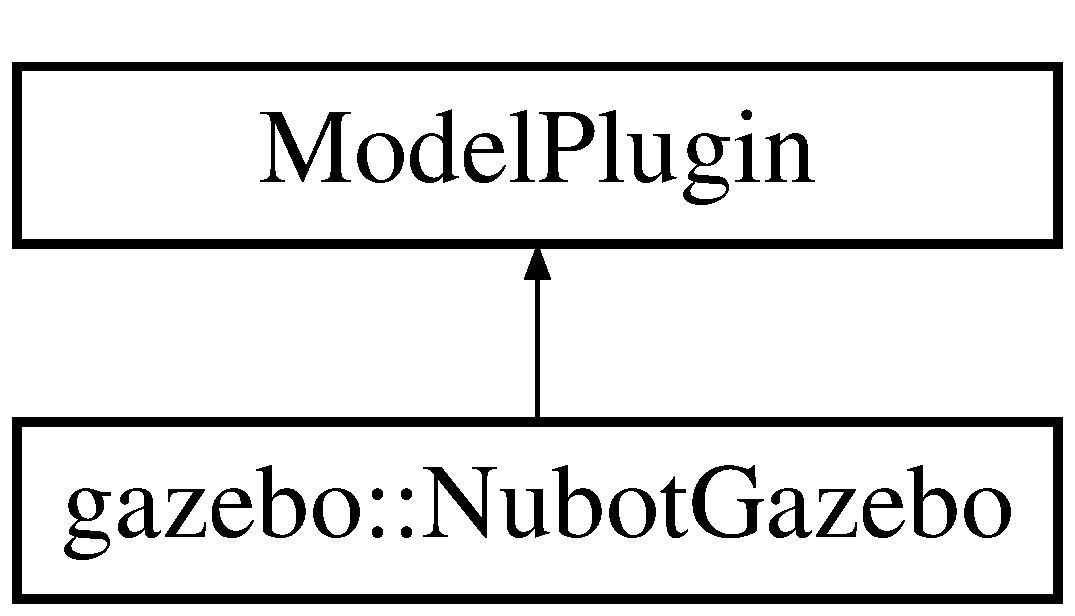
\includegraphics[height=2.000000cm]{classgazebo_1_1NubotGazebo}
\end{center}
\end{figure}
\subsection*{Public Member Functions}
\begin{DoxyCompactItemize}
\item 
\hyperlink{classgazebo_1_1NubotGazebo_a6c8d0be666316dfa03c49ec0a5e01e96}{Nubot\-Gazebo} ()
\begin{DoxyCompactList}\small\item\em Constructor. Will be called firstly. \end{DoxyCompactList}\item 
virtual \hyperlink{classgazebo_1_1NubotGazebo_a90ec014dbd4dcad3f1f0c78771fd4e63}{$\sim$\-Nubot\-Gazebo} ()
\begin{DoxyCompactList}\small\item\em Destructor. \end{DoxyCompactList}\end{DoxyCompactItemize}
\subsection*{Protected Member Functions}
\begin{DoxyCompactItemize}
\item 
void \hyperlink{classgazebo_1_1NubotGazebo_aa1eea79757774a935fe82a5fbc1b3f94}{Load} (physics\-::\-Model\-Ptr \-\_\-parent, sdf\-::\-Element\-Ptr)
\begin{DoxyCompactList}\small\item\em Load the controller. Required by model plugin. Will be called secondly. \end{DoxyCompactList}\item 
virtual void \hyperlink{classgazebo_1_1NubotGazebo_a9d2bb8130da6d209089f5ee469427ca4}{Update\-Child} ()
\begin{DoxyCompactList}\small\item\em Update the controller. It is running every simulation iteration. So you can put your core code here.(in this code, either \hyperlink{classgazebo_1_1NubotGazebo_aaa7835337bbfd120b5b85af40ccf47ae}{nubot\-\_\-be\-\_\-control()} or \hyperlink{classgazebo_1_1NubotGazebo_a991cc13697cbd1eaf855d21e4f5d78d2}{nubot\-\_\-auto\-\_\-control()}) \end{DoxyCompactList}\item 
virtual void \hyperlink{classgazebo_1_1NubotGazebo_abf91360d6ce9b5f2cf02c3907100495e}{Init} ()
\begin{DoxyCompactList}\small\item\em Model Initialization(after the Load function). Not required by model plugin. Will be called thirdly. \end{DoxyCompactList}\item 
virtual void \hyperlink{classgazebo_1_1NubotGazebo_aefa336771bb8dffca92a2919352b62bc}{Reset} ()
\begin{DoxyCompactList}\small\item\em Model Reset function. Not required by model plugin. It is triggered when the world resets. \end{DoxyCompactList}\end{DoxyCompactItemize}
\subsection*{Private Member Functions}
\begin{DoxyCompactItemize}
\item 
void \hyperlink{classgazebo_1_1NubotGazebo_a96b102bf11d96dda2cdab0f2f9460d8d}{model\-\_\-states\-\_\-\-C\-B} (const gazebo\-\_\-msgs\-::\-Model\-States\-::\-Const\-Ptr \&\-\_\-msg)
\begin{DoxyCompactList}\small\item\em Model\-States message callback function. \end{DoxyCompactList}\item 
void \hyperlink{classgazebo_1_1NubotGazebo_aafe5e8deca0e5a85a30c73629eee8703}{vel\-\_\-cmd\-\_\-\-C\-B} (const \hyperlink{structnubot__common_1_1VelCmd___a5a57f1d76c9209090962bf805a6d8cc8}{nubot\-\_\-common\-::\-Vel\-Cmd\-::\-Const\-Ptr} \&cmd)
\begin{DoxyCompactList}\small\item\em Vel\-Cmd message callback function. \end{DoxyCompactList}\item 
bool \hyperlink{classgazebo_1_1NubotGazebo_ae042db5614aea3da7c8f547c44d9ff6e}{ball\-\_\-handle\-\_\-control\-\_\-service} (\hyperlink{structnubot__common_1_1BallHandle_a02af01a2f731b0fc249f1cf9df23a00e}{nubot\-\_\-common\-::\-Ball\-Handle\-::\-Request} \&req, \hyperlink{structnubot__common_1_1BallHandle_a6c4cc1c333d5fe1cfc569ee22b68ba89}{nubot\-\_\-common\-::\-Ball\-Handle\-::\-Response} \&res)
\begin{DoxyCompactList}\small\item\em Ball handling service server function. \end{DoxyCompactList}\item 
bool \hyperlink{classgazebo_1_1NubotGazebo_ade096537ecc11263f1dd14428325329b}{shoot\-\_\-control\-\_\-servive} (\hyperlink{structnubot__common_1_1Shoot_a8d200603298d1fe7377f13911e7d5bdc}{nubot\-\_\-common\-::\-Shoot\-::\-Request} \&req, \hyperlink{structnubot__common_1_1Shoot_a4d609a5e9faac9c7c0d32b7cf0eb5738}{nubot\-\_\-common\-::\-Shoot\-::\-Response} \&res)
\begin{DoxyCompactList}\small\item\em Ball shooting service server function. \end{DoxyCompactList}\item 
void \hyperlink{classgazebo_1_1NubotGazebo_a2c87fbf2e13762d4827367028d493670}{message\-\_\-queue\-\_\-thread} ()
\begin{DoxyCompactList}\small\item\em Custom message callback queue thread. \end{DoxyCompactList}\item 
void \hyperlink{classgazebo_1_1NubotGazebo_abe786a1fbc3407f1b2ac655b1af15a8b}{service\-\_\-queue\-\_\-thread} ()
\begin{DoxyCompactList}\small\item\em Custom service callback queue thread. \end{DoxyCompactList}\item 
bool \hyperlink{classgazebo_1_1NubotGazebo_a3b884175db3fd9e7ac88f6076d5f2b8e}{update\-\_\-model\-\_\-info} (void)
\begin{DoxyCompactList}\small\item\em Updating models' states; By default, Gaussian noise is not added, but you can add it by changing the flag in this function. \end{DoxyCompactList}\item 
void \hyperlink{classgazebo_1_1NubotGazebo_ad93752507f23724bba2f731325e4c14b}{nubot\-\_\-locomotion} (math\-::\-Vector3 linear\-\_\-vel\-\_\-vector, math\-::\-Vector3 angular\-\_\-vel\-\_\-vector)
\begin{DoxyCompactList}\small\item\em Nubot moving fuction\-: rotation + translation. \end{DoxyCompactList}\item 
bool \hyperlink{classgazebo_1_1NubotGazebo_a8ac8c9467b8e14b4ceb0718d97031617}{get\-\_\-rot\-\_\-vector} (math\-::\-Vector3 target\-\_\-point\-\_\-world, double degree\-\_\-thres)
\begin{DoxyCompactList}\small\item\em Nubot rotates; kicking mechanism towards ball. \end{DoxyCompactList}\item 
bool \hyperlink{classgazebo_1_1NubotGazebo_a0a50fbb4be79c99cf860b84413f8fa9b}{get\-\_\-trans\-\_\-vector} (math\-::\-Vector3 target\-\_\-point\-\_\-world, double metre\-\_\-thres)
\begin{DoxyCompactList}\small\item\em Nubot chasing football function. \end{DoxyCompactList}\item 
void \hyperlink{classgazebo_1_1NubotGazebo_a91862269320f78bc24856e8877af3cc4}{dribble\-\_\-ball} (void)
\begin{DoxyCompactList}\small\item\em Nubot dribbling ball function. The football follows nubot movement. \end{DoxyCompactList}\item 
void \hyperlink{classgazebo_1_1NubotGazebo_a0b8f02255ccde5f6768afb45fee8b81b}{kick\-\_\-ball} (int mode, double vel)
\begin{DoxyCompactList}\small\item\em Nubot kicking ball. For more information, read the paper \char`\"{}\-Weijia Yao et al., A Simulation System Based on R\-O\-S and Gazebo for Robo\-Cup Middle Size League, 2015\char`\"{}. \end{DoxyCompactList}\item 
bool \hyperlink{classgazebo_1_1NubotGazebo_a8366f268f6bba085201123d74b786368}{get\-\_\-is\-\_\-hold\-\_\-ball} (void)
\begin{DoxyCompactList}\small\item\em Get the value of flag is\-\_\-hold\-\_\-ball\-\_\-. \end{DoxyCompactList}\item 
void \hyperlink{classgazebo_1_1NubotGazebo_a991cc13697cbd1eaf855d21e4f5d78d2}{nubot\-\_\-auto\-\_\-control} (void)
\begin{DoxyCompactList}\small\item\em Single nubot predefined autonomous motions. \end{DoxyCompactList}\item 
void \hyperlink{classgazebo_1_1NubotGazebo_aaa7835337bbfd120b5b85af40ccf47ae}{nubot\-\_\-be\-\_\-control} (void)
\begin{DoxyCompactList}\small\item\em Robot motion controlled by real-\/robot code; or controlled by a keyboard. \end{DoxyCompactList}\item 
void \hyperlink{classgazebo_1_1NubotGazebo_a828269281839a4f18d30f02d20ad62b6}{config} (\hyperlink{classnubot__gazebo_1_1NubotGazeboConfig}{nubot\-\_\-gazebo\-::\-Nubot\-Gazebo\-Config} \&config, uint32\-\_\-t level)
\begin{DoxyCompactList}\small\item\em dynmaic recofigure calback function \end{DoxyCompactList}\item 
void \hyperlink{classgazebo_1_1NubotGazebo_a3a42f8965b7ccb35d0b6a0624c56ba86}{ball\-\_\-vel\-\_\-decay} (math\-::\-Vector3 vel, double mu)
\begin{DoxyCompactList}\small\item\em a work-\/around for no rolling-\/friction in O\-D\-E. For more information, please read O\-D\-E manual. \end{DoxyCompactList}\item 
void \hyperlink{classgazebo_1_1NubotGazebo_a5b5d4a3644867257cb379613072e9567}{set\-\_\-ball\-\_\-vel} (math\-::\-Vector3 \&vel, bool \&ball\-\_\-decay\-\_\-flag)
\begin{DoxyCompactList}\small\item\em replace football\-\_\-model\-\_\--\/$>$Set\-Linear\-Vel() with a flag to indicate vel decay \end{DoxyCompactList}\end{DoxyCompactItemize}
\subsection*{Private Attributes}
\begin{DoxyCompactItemize}
\item 
physics\-::\-World\-Ptr \hyperlink{classgazebo_1_1NubotGazebo_aa56e5c10cfbbc981460ab1bcc204d071}{world\-\_\-}
\item 
physics\-::\-Model\-Ptr \hyperlink{classgazebo_1_1NubotGazebo_ac7f22b4b498327d11697f07cb064e460}{nubot\-\_\-model\-\_\-}
\item 
physics\-::\-Model\-Ptr \hyperlink{classgazebo_1_1NubotGazebo_a76897836db2bb2e49c75fbf64b4b9aeb}{football\-\_\-model\-\_\-}
\item 
physics\-::\-Link\-Ptr \hyperlink{classgazebo_1_1NubotGazebo_a191e11ef5a0b3e6275c3938ad61cec0a}{football\-\_\-link\-\_\-}
\item 
physics\-::\-Link\-Ptr \hyperlink{classgazebo_1_1NubotGazebo_a97a021a147d45134fe79ab21531e55df}{nubot\-\_\-link\-\_\-}
\item 
ros\-::\-Node\-Handle $\ast$ \hyperlink{classgazebo_1_1NubotGazebo_a310c7df239fab0570dbdc82d4552ec6d}{rosnode\-\_\-}
\item 
ros\-::\-Subscriber \hyperlink{classgazebo_1_1NubotGazebo_a7b758780795b0406d06bf5db5122dbe2}{Model\-States\-\_\-sub\-\_\-}
\item 
ros\-::\-Subscriber \hyperlink{classgazebo_1_1NubotGazebo_a6264896320559e214ac33d820c44b357}{Velcmd\-\_\-sub\-\_\-}
\item 
ros\-::\-Service\-Server \hyperlink{classgazebo_1_1NubotGazebo_af8abc682c8dc7cad7d29d131901aec05}{ballhandle\-\_\-server\-\_\-}
\item 
ros\-::\-Service\-Server \hyperlink{classgazebo_1_1NubotGazebo_afd3e6ab82580823e83d84433dac19e86}{shoot\-\_\-server\-\_\-}
\item 
boost\-::thread \hyperlink{classgazebo_1_1NubotGazebo_ae985620428222dd9b1b5f507339119b8}{message\-\_\-callback\-\_\-queue\-\_\-thread\-\_\-}
\item 
boost\-::thread \hyperlink{classgazebo_1_1NubotGazebo_a0c0bc3e99d501d7fcac319848006f87c}{service\-\_\-callback\-\_\-queue\-\_\-thread\-\_\-}
\item 
boost\-::mutex \hyperlink{classgazebo_1_1NubotGazebo_a70f7775e1670311efc2aad7c306a3077}{msg\-C\-B\-\_\-lock\-\_\-}
\item 
boost\-::mutex \hyperlink{classgazebo_1_1NubotGazebo_a6b3d2a253732eedfcf18e0223435bed0}{srv\-C\-B\-\_\-lock\-\_\-}
\item 
ros\-::\-Callback\-Queue \hyperlink{classgazebo_1_1NubotGazebo_a7186c914f81602db7bd347b940794bbf}{message\-\_\-queue\-\_\-}
\item 
ros\-::\-Callback\-Queue \hyperlink{classgazebo_1_1NubotGazebo_ae1fe2dc1962659f70ebba9555a92e59a}{service\-\_\-queue\-\_\-}
\item 
event\-::\-Connection\-Ptr \hyperlink{classgazebo_1_1NubotGazebo_a4e3b8b74aa075427ecbd5c82f630144d}{update\-\_\-connection\-\_\-}
\item 
gazebo\-\_\-msgs\-::\-Model\-States \hyperlink{classgazebo_1_1NubotGazebo_a320dc212fab523958abb529f946133bd}{model\-\_\-states\-\_\-msg\-\_\-}
\item 
\hyperlink{structgazebo_1_1model__state}{model\-\_\-state} \hyperlink{classgazebo_1_1NubotGazebo_a5abf5be34d8441db05d94ead7924ce14}{nubot\-\_\-state\-\_\-}
\item 
\hyperlink{structgazebo_1_1model__state}{model\-\_\-state} \hyperlink{classgazebo_1_1NubotGazebo_af7356a83d30997d884440a10e95d29f4}{football\-\_\-state\-\_\-}
\item 
common\-::\-Time \hyperlink{classgazebo_1_1NubotGazebo_a36186a24f60f3c88fd6fb12fd85b4fa4}{receive\-\_\-sim\-\_\-time\-\_\-}
\item 
common\-::\-Time \hyperlink{classgazebo_1_1NubotGazebo_a8e05ad53365765db200e0d62c451e069}{last\-\_\-current\-\_\-time\-\_\-}
\item 
math\-::\-Vector3 \hyperlink{classgazebo_1_1NubotGazebo_a385577ffa9cc48440e8047019d6e67f6}{desired\-\_\-rot\-\_\-vector\-\_\-}
\item 
math\-::\-Vector3 \hyperlink{classgazebo_1_1NubotGazebo_ac515996ccf0c682a0ed88f00e401373d}{desired\-\_\-trans\-\_\-vector\-\_\-}
\item 
math\-::\-Vector3 \hyperlink{classgazebo_1_1NubotGazebo_ae4b4790d24996fbfdd51f74baa45170a}{nubot\-\_\-football\-\_\-vector\-\_\-}
\item 
math\-::\-Vector3 \hyperlink{classgazebo_1_1NubotGazebo_aea8b62919e2834d4311a7fd7935036af}{kick\-\_\-vector\-\_\-world\-\_\-}
\item 
double \hyperlink{classgazebo_1_1NubotGazebo_a11fbfac7f239d13730b4d676af18f67e}{nubot\-\_\-football\-\_\-vector\-\_\-length\-\_\-}
\item 
std\-::string \hyperlink{classgazebo_1_1NubotGazebo_ac92e4461911d9522f1454978d26ec461}{robot\-\_\-namespace\-\_\-}
\item 
std\-::string \hyperlink{classgazebo_1_1NubotGazebo_adf2314dfb2ab6cb5ecdb2bb0a9736665}{model\-\_\-name\-\_\-}
\item 
std\-::string \hyperlink{classgazebo_1_1NubotGazebo_aea004ec0ee1c5dfdc8cba31939f18e39}{football\-\_\-name\-\_\-}
\item 
std\-::string \hyperlink{classgazebo_1_1NubotGazebo_a918fab93f4939a8bb06d65a997e20a54}{football\-\_\-chassis\-\_\-}
\item 
std\-::string \hyperlink{classgazebo_1_1NubotGazebo_a5d3cf2ace05ce1ade8b71d1c6397a7b0}{robot\-\_\-prefix\-\_\-}
\item 
unsigned int \hyperlink{classgazebo_1_1NubotGazebo_af45b036c2156b537d5282f63c509d1e4}{football\-\_\-index\-\_\-}
\item 
unsigned int \hyperlink{classgazebo_1_1NubotGazebo_adce69b7247cba8a3433a6cdfad5b61ef}{nubot\-\_\-index\-\_\-}
\item 
double \hyperlink{classgazebo_1_1NubotGazebo_a67f7850c63c5dd6fe80694c9a426e5ec}{max\-\_\-linear\-\_\-vel\-\_\-}
\item 
double \hyperlink{classgazebo_1_1NubotGazebo_ae9da5f6a1c7b5624dbf6bb20a2819d40}{max\-\_\-angular\-\_\-vel\-\_\-}
\item 
double \hyperlink{classgazebo_1_1NubotGazebo_a646a80199e35f2f47558b7b7aa27bea4}{dribble\-\_\-distance\-\_\-thres\-\_\-}
\item 
double \hyperlink{classgazebo_1_1NubotGazebo_ab012e0229172416640558cf2746a0974}{dribble\-\_\-angle\-\_\-thres\-\_\-}
\item 
double \hyperlink{classgazebo_1_1NubotGazebo_abc8f7cb67014e700c08e27023353e419}{kick\-\_\-ball\-\_\-vel\-\_\-}
\item 
double \hyperlink{classgazebo_1_1NubotGazebo_af17747304ff9b241fa0642c52923498b}{Vx\-\_\-cmd\-\_\-}
\item 
double \hyperlink{classgazebo_1_1NubotGazebo_a977c91e62fed23c5fb9233e5d38ad597}{Vy\-\_\-cmd\-\_\-}
\item 
double \hyperlink{classgazebo_1_1NubotGazebo_aebc0851c9ab6da1d1c96d470e72758f8}{w\-\_\-cmd\-\_\-}
\item 
double \hyperlink{classgazebo_1_1NubotGazebo_a7ebd21f6da11a8f2b514c2e0930a26e6}{force\-\_\-}
\item 
double \hyperlink{classgazebo_1_1NubotGazebo_a9e30363181d0a790081ce6d0e9151e6b}{dribble\-\_\-\-P\-\_\-}
\item 
double \hyperlink{classgazebo_1_1NubotGazebo_ab74f3e63fe906f0c982837b1eeeefb5c}{dribble\-\_\-\-I\-\_\-}
\item 
double \hyperlink{classgazebo_1_1NubotGazebo_a727079312e073df8799e1a385ac8da00}{dribble\-\_\-\-D\-\_\-}
\item 
double \hyperlink{classgazebo_1_1NubotGazebo_a0f8a50e34877912a0c53c3185ccd28d9}{I\-\_\-term\-\_\-max\-\_\-}
\item 
double \hyperlink{classgazebo_1_1NubotGazebo_affe0d982594c738a7ebec3ac1849c01f}{I\-\_\-term\-\_\-min\-\_\-}
\item 
double \hyperlink{classgazebo_1_1NubotGazebo_a6b6ab10ac24ec1483797885f5d1b9110}{cmd\-\_\-max\-\_\-}
\item 
double \hyperlink{classgazebo_1_1NubotGazebo_a360cbab192432814122197f21d685e56}{cmd\-\_\-min\-\_\-}
\item 
int \hyperlink{classgazebo_1_1NubotGazebo_a3c54a29f7aa4e67e4f86b5e848a930d5}{mode\-\_\-}
\item 
common\-::\-Time \hyperlink{classgazebo_1_1NubotGazebo_a1aeb8fee9f7e057b182afcf2fd03f1c1}{last\-\_\-update\-\_\-time\-\_\-}
\item 
unsigned int \hyperlink{classgazebo_1_1NubotGazebo_aefc2d91922066c5ffc1d7faa175ab68a}{model\-\_\-count\-\_\-}
\item 
bool \hyperlink{classgazebo_1_1NubotGazebo_a408738f621515f00547b54ed74481127}{dribble\-\_\-flag\-\_\-}
\item 
bool \hyperlink{classgazebo_1_1NubotGazebo_a85d5357dfacc73801bed752d6dc297d4}{shot\-\_\-flag\-\_\-}
\item 
bool \hyperlink{classgazebo_1_1NubotGazebo_ae7c8ddd9342426222c1354740b23a01d}{Model\-States\-C\-B\-\_\-flag\-\_\-}
\item 
bool \hyperlink{classgazebo_1_1NubotGazebo_a6392423c1aaf2ba68aac9eeb318f9e5b}{judge\-\_\-nubot\-\_\-stuck\-\_\-}
\item 
bool \hyperlink{classgazebo_1_1NubotGazebo_a0d63b5e7f3d213fca30bbe09bd15e114}{is\-\_\-hold\-\_\-ball\-\_\-}
\item 
bool \hyperlink{classgazebo_1_1NubotGazebo_a51c8eaa9e931b22700f6c000e413bfa2}{ball\-\_\-decay\-\_\-flag\-\_\-}
\item 
int \hyperlink{classgazebo_1_1NubotGazebo_afbdb7428487c2f6dec5000bae3d6f5a7}{count\-\_\-}
\item 
\hyperlink{nubot__gazebo_8hh_a9f17572284bab3e9bd067a6393a7953b}{nubot\-\_\-state} \hyperlink{classgazebo_1_1NubotGazebo_acf9828d7b8b37440a8e45ef63895ec8b}{state\-\_\-}
\item 
\hyperlink{nubot__gazebo_8hh_a503a2f01f9f49bd293d3c44faf21b528}{nubot\-\_\-substate} \hyperlink{classgazebo_1_1NubotGazebo_a8db3f4b9767b4ec34716756f02fb7fe9}{sub\-\_\-state\-\_\-}
\item 
\hyperlink{classnubot_1_1PID}{nubot\-::\-P\-I\-D} \hyperlink{classgazebo_1_1NubotGazebo_a5865f8d5f7aad90ace72fe2942b6d25e}{dribble\-\_\-pid\-\_\-}
\item 
\hyperlink{classnubot_1_1ParaTrajPlanning}{nubot\-::\-Para\-Traj\-Planning} \hyperlink{classgazebo_1_1NubotGazebo_ac16bd419aba2826c0227ac575b351e9e}{traj\-\_\-plan\-\_\-linear\-\_\-}
\item 
\hyperlink{classnubot_1_1ParaTrajPlanning}{nubot\-::\-Para\-Traj\-Planning} \hyperlink{classgazebo_1_1NubotGazebo_a95c171c478be4aadf6b4d96a3d3a48c8}{traj\-\_\-plan\-\_\-rot\-\_\-}
\item 
math\-::\-Rand \hyperlink{classgazebo_1_1NubotGazebo_a5a6b999a205a45e1778e0f4d75e325e0}{rand\-\_\-}
\item 
dynamic\-\_\-reconfigure\-::\-Server\\*
$<$ \hyperlink{classnubot__gazebo_1_1NubotGazeboConfig}{nubot\-\_\-gazebo\-::\-Nubot\-Gazebo\-Config} $>$ $\ast$ \hyperlink{classgazebo_1_1NubotGazebo_a6f892f9dcb5b46bdd232ffec277dd093}{reconfigure\-Server\-\_\-}
\end{DoxyCompactItemize}


\subsection{Detailed Description}
A basic motions realization in Gazebo. 

\subsection{Constructor \& Destructor Documentation}
\hypertarget{classgazebo_1_1NubotGazebo_a6c8d0be666316dfa03c49ec0a5e01e96}{\index{gazebo\-::\-Nubot\-Gazebo@{gazebo\-::\-Nubot\-Gazebo}!Nubot\-Gazebo@{Nubot\-Gazebo}}
\index{Nubot\-Gazebo@{Nubot\-Gazebo}!gazebo::NubotGazebo@{gazebo\-::\-Nubot\-Gazebo}}
\subsubsection[{Nubot\-Gazebo}]{\setlength{\rightskip}{0pt plus 5cm}Nubot\-Gazebo\-::\-Nubot\-Gazebo (
\begin{DoxyParamCaption}
{}
\end{DoxyParamCaption}
)}}\label{classgazebo_1_1NubotGazebo_a6c8d0be666316dfa03c49ec0a5e01e96}


Constructor. Will be called firstly. 

\hypertarget{classgazebo_1_1NubotGazebo_a90ec014dbd4dcad3f1f0c78771fd4e63}{\index{gazebo\-::\-Nubot\-Gazebo@{gazebo\-::\-Nubot\-Gazebo}!$\sim$\-Nubot\-Gazebo@{$\sim$\-Nubot\-Gazebo}}
\index{$\sim$\-Nubot\-Gazebo@{$\sim$\-Nubot\-Gazebo}!gazebo::NubotGazebo@{gazebo\-::\-Nubot\-Gazebo}}
\subsubsection[{$\sim$\-Nubot\-Gazebo}]{\setlength{\rightskip}{0pt plus 5cm}Nubot\-Gazebo\-::$\sim$\-Nubot\-Gazebo (
\begin{DoxyParamCaption}
{}
\end{DoxyParamCaption}
)\hspace{0.3cm}{\ttfamily [virtual]}}}\label{classgazebo_1_1NubotGazebo_a90ec014dbd4dcad3f1f0c78771fd4e63}


Destructor. 



\subsection{Member Function Documentation}
\hypertarget{classgazebo_1_1NubotGazebo_ae042db5614aea3da7c8f547c44d9ff6e}{\index{gazebo\-::\-Nubot\-Gazebo@{gazebo\-::\-Nubot\-Gazebo}!ball\-\_\-handle\-\_\-control\-\_\-service@{ball\-\_\-handle\-\_\-control\-\_\-service}}
\index{ball\-\_\-handle\-\_\-control\-\_\-service@{ball\-\_\-handle\-\_\-control\-\_\-service}!gazebo::NubotGazebo@{gazebo\-::\-Nubot\-Gazebo}}
\subsubsection[{ball\-\_\-handle\-\_\-control\-\_\-service}]{\setlength{\rightskip}{0pt plus 5cm}bool Nubot\-Gazebo\-::ball\-\_\-handle\-\_\-control\-\_\-service (
\begin{DoxyParamCaption}
\item[{{\bf nubot\-\_\-common\-::\-Ball\-Handle\-::\-Request} \&}]{req, }
\item[{{\bf nubot\-\_\-common\-::\-Ball\-Handle\-::\-Response} \&}]{res}
\end{DoxyParamCaption}
)\hspace{0.3cm}{\ttfamily [private]}}}\label{classgazebo_1_1NubotGazebo_ae042db5614aea3da7c8f547c44d9ff6e}


Ball handling service server function. 


\begin{DoxyParams}[1]{Parameters}
\mbox{\tt in}  & {\em req} & ball handle service request \\
\hline
\mbox{\tt out}  & {\em res} & ball handle service response \\
\hline
\end{DoxyParams}
\hypertarget{classgazebo_1_1NubotGazebo_a3a42f8965b7ccb35d0b6a0624c56ba86}{\index{gazebo\-::\-Nubot\-Gazebo@{gazebo\-::\-Nubot\-Gazebo}!ball\-\_\-vel\-\_\-decay@{ball\-\_\-vel\-\_\-decay}}
\index{ball\-\_\-vel\-\_\-decay@{ball\-\_\-vel\-\_\-decay}!gazebo::NubotGazebo@{gazebo\-::\-Nubot\-Gazebo}}
\subsubsection[{ball\-\_\-vel\-\_\-decay}]{\setlength{\rightskip}{0pt plus 5cm}void Nubot\-Gazebo\-::ball\-\_\-vel\-\_\-decay (
\begin{DoxyParamCaption}
\item[{math\-::\-Vector3}]{vel, }
\item[{double}]{mu}
\end{DoxyParamCaption}
)\hspace{0.3cm}{\ttfamily [private]}}}\label{classgazebo_1_1NubotGazebo_a3a42f8965b7ccb35d0b6a0624c56ba86}


a work-\/around for no rolling-\/friction in O\-D\-E. For more information, please read O\-D\-E manual. 


\begin{DoxyParams}[1]{Parameters}
\mbox{\tt in}  & {\em vel} & football's current 3\-D velocity \\
\hline
\mbox{\tt in}  & {\em mu} & friction coefficient \\
\hline
\end{DoxyParams}
\hypertarget{classgazebo_1_1NubotGazebo_a828269281839a4f18d30f02d20ad62b6}{\index{gazebo\-::\-Nubot\-Gazebo@{gazebo\-::\-Nubot\-Gazebo}!config@{config}}
\index{config@{config}!gazebo::NubotGazebo@{gazebo\-::\-Nubot\-Gazebo}}
\subsubsection[{config}]{\setlength{\rightskip}{0pt plus 5cm}void Nubot\-Gazebo\-::config (
\begin{DoxyParamCaption}
\item[{{\bf nubot\-\_\-gazebo\-::\-Nubot\-Gazebo\-Config} \&}]{config, }
\item[{uint32\-\_\-t}]{level}
\end{DoxyParamCaption}
)\hspace{0.3cm}{\ttfamily [private]}}}\label{classgazebo_1_1NubotGazebo_a828269281839a4f18d30f02d20ad62b6}


dynmaic recofigure calback function 

\hypertarget{classgazebo_1_1NubotGazebo_a91862269320f78bc24856e8877af3cc4}{\index{gazebo\-::\-Nubot\-Gazebo@{gazebo\-::\-Nubot\-Gazebo}!dribble\-\_\-ball@{dribble\-\_\-ball}}
\index{dribble\-\_\-ball@{dribble\-\_\-ball}!gazebo::NubotGazebo@{gazebo\-::\-Nubot\-Gazebo}}
\subsubsection[{dribble\-\_\-ball}]{\setlength{\rightskip}{0pt plus 5cm}void Nubot\-Gazebo\-::dribble\-\_\-ball (
\begin{DoxyParamCaption}
\item[{void}]{}
\end{DoxyParamCaption}
)\hspace{0.3cm}{\ttfamily [private]}}}\label{classgazebo_1_1NubotGazebo_a91862269320f78bc24856e8877af3cc4}


Nubot dribbling ball function. The football follows nubot movement. 

Three ways of ball-\/dribbling are provided\-: 1. Set ball pose;
\begin{DoxyEnumerate}
\item Set tangential velocity; 3. Set secant velocity. 
\end{DoxyEnumerate}\hypertarget{classgazebo_1_1NubotGazebo_a8366f268f6bba085201123d74b786368}{\index{gazebo\-::\-Nubot\-Gazebo@{gazebo\-::\-Nubot\-Gazebo}!get\-\_\-is\-\_\-hold\-\_\-ball@{get\-\_\-is\-\_\-hold\-\_\-ball}}
\index{get\-\_\-is\-\_\-hold\-\_\-ball@{get\-\_\-is\-\_\-hold\-\_\-ball}!gazebo::NubotGazebo@{gazebo\-::\-Nubot\-Gazebo}}
\subsubsection[{get\-\_\-is\-\_\-hold\-\_\-ball}]{\setlength{\rightskip}{0pt plus 5cm}bool Nubot\-Gazebo\-::get\-\_\-is\-\_\-hold\-\_\-ball (
\begin{DoxyParamCaption}
\item[{void}]{}
\end{DoxyParamCaption}
)\hspace{0.3cm}{\ttfamily [private]}}}\label{classgazebo_1_1NubotGazebo_a8366f268f6bba085201123d74b786368}


Get the value of flag is\-\_\-hold\-\_\-ball\-\_\-. 

\begin{DoxyReturn}{Returns}
1\-: is holding ball 0\-: is not holding ball 
\end{DoxyReturn}
\hypertarget{classgazebo_1_1NubotGazebo_a8ac8c9467b8e14b4ceb0718d97031617}{\index{gazebo\-::\-Nubot\-Gazebo@{gazebo\-::\-Nubot\-Gazebo}!get\-\_\-rot\-\_\-vector@{get\-\_\-rot\-\_\-vector}}
\index{get\-\_\-rot\-\_\-vector@{get\-\_\-rot\-\_\-vector}!gazebo::NubotGazebo@{gazebo\-::\-Nubot\-Gazebo}}
\subsubsection[{get\-\_\-rot\-\_\-vector}]{\setlength{\rightskip}{0pt plus 5cm}bool Nubot\-Gazebo\-::get\-\_\-rot\-\_\-vector (
\begin{DoxyParamCaption}
\item[{math\-::\-Vector3}]{target\-\_\-point\-\_\-world, }
\item[{double}]{degree\-\_\-thres}
\end{DoxyParamCaption}
)\hspace{0.3cm}{\ttfamily [private]}}}\label{classgazebo_1_1NubotGazebo_a8ac8c9467b8e14b4ceb0718d97031617}


Nubot rotates; kicking mechanism towards ball. 


\begin{DoxyParams}[1]{Parameters}
\mbox{\tt in}  & {\em target\-\_\-point\-\_\-world} & target point coordinates in world frame \\
\hline
\mbox{\tt in}  & {\em degree\-\_\-thres} & angle error threshold in degree \\
\hline
\end{DoxyParams}
\begin{DoxyReturn}{Returns}
bool value indicate if reach the target orientation. 1\-: yes; 0\-:no 
\end{DoxyReturn}
\hypertarget{classgazebo_1_1NubotGazebo_a0a50fbb4be79c99cf860b84413f8fa9b}{\index{gazebo\-::\-Nubot\-Gazebo@{gazebo\-::\-Nubot\-Gazebo}!get\-\_\-trans\-\_\-vector@{get\-\_\-trans\-\_\-vector}}
\index{get\-\_\-trans\-\_\-vector@{get\-\_\-trans\-\_\-vector}!gazebo::NubotGazebo@{gazebo\-::\-Nubot\-Gazebo}}
\subsubsection[{get\-\_\-trans\-\_\-vector}]{\setlength{\rightskip}{0pt plus 5cm}bool Nubot\-Gazebo\-::get\-\_\-trans\-\_\-vector (
\begin{DoxyParamCaption}
\item[{math\-::\-Vector3}]{target\-\_\-point\-\_\-world, }
\item[{double}]{metre\-\_\-thres}
\end{DoxyParamCaption}
)\hspace{0.3cm}{\ttfamily [private]}}}\label{classgazebo_1_1NubotGazebo_a0a50fbb4be79c99cf860b84413f8fa9b}


Nubot chasing football function. 


\begin{DoxyParams}[1]{Parameters}
\mbox{\tt in}  & {\em target\-\_\-point\-\_\-world} & target point coordinates in world frame \\
\hline
\mbox{\tt in}  & {\em metre\-\_\-thres} & distance error threshold in metres \\
\hline
\end{DoxyParams}
\begin{DoxyReturn}{Returns}
bool value indicate if reach the target position. 1\-:yes; 0\-:no 
\end{DoxyReturn}
\hypertarget{classgazebo_1_1NubotGazebo_abf91360d6ce9b5f2cf02c3907100495e}{\index{gazebo\-::\-Nubot\-Gazebo@{gazebo\-::\-Nubot\-Gazebo}!Init@{Init}}
\index{Init@{Init}!gazebo::NubotGazebo@{gazebo\-::\-Nubot\-Gazebo}}
\subsubsection[{Init}]{\setlength{\rightskip}{0pt plus 5cm}void Nubot\-Gazebo\-::\-Init (
\begin{DoxyParamCaption}
{}
\end{DoxyParamCaption}
)\hspace{0.3cm}{\ttfamily [protected]}, {\ttfamily [virtual]}}}\label{classgazebo_1_1NubotGazebo_abf91360d6ce9b5f2cf02c3907100495e}


Model Initialization(after the Load function). Not required by model plugin. Will be called thirdly. 

\hypertarget{classgazebo_1_1NubotGazebo_a0b8f02255ccde5f6768afb45fee8b81b}{\index{gazebo\-::\-Nubot\-Gazebo@{gazebo\-::\-Nubot\-Gazebo}!kick\-\_\-ball@{kick\-\_\-ball}}
\index{kick\-\_\-ball@{kick\-\_\-ball}!gazebo::NubotGazebo@{gazebo\-::\-Nubot\-Gazebo}}
\subsubsection[{kick\-\_\-ball}]{\setlength{\rightskip}{0pt plus 5cm}void Nubot\-Gazebo\-::kick\-\_\-ball (
\begin{DoxyParamCaption}
\item[{int}]{mode, }
\item[{double}]{vel = {\ttfamily 20.0}}
\end{DoxyParamCaption}
)\hspace{0.3cm}{\ttfamily [private]}}}\label{classgazebo_1_1NubotGazebo_a0b8f02255ccde5f6768afb45fee8b81b}


Nubot kicking ball. For more information, read the paper \char`\"{}\-Weijia Yao et al., A Simulation System Based on R\-O\-S and Gazebo for Robo\-Cup Middle Size League, 2015\char`\"{}. 


\begin{DoxyParams}[1]{Parameters}
\mbox{\tt in}  & {\em mode} & kick ball mode F\-L\-Y or R\-U\-N \\
\hline
\mbox{\tt in}  & {\em vel} & initial velocity of the ball kicked \\
\hline
\end{DoxyParams}
\hypertarget{classgazebo_1_1NubotGazebo_aa1eea79757774a935fe82a5fbc1b3f94}{\index{gazebo\-::\-Nubot\-Gazebo@{gazebo\-::\-Nubot\-Gazebo}!Load@{Load}}
\index{Load@{Load}!gazebo::NubotGazebo@{gazebo\-::\-Nubot\-Gazebo}}
\subsubsection[{Load}]{\setlength{\rightskip}{0pt plus 5cm}void Nubot\-Gazebo\-::\-Load (
\begin{DoxyParamCaption}
\item[{physics\-::\-Model\-Ptr}]{\-\_\-parent, }
\item[{sdf\-::\-Element\-Ptr}]{\-\_\-sdf}
\end{DoxyParamCaption}
)\hspace{0.3cm}{\ttfamily [protected]}}}\label{classgazebo_1_1NubotGazebo_aa1eea79757774a935fe82a5fbc1b3f94}


Load the controller. Required by model plugin. Will be called secondly. 

\hypertarget{classgazebo_1_1NubotGazebo_a2c87fbf2e13762d4827367028d493670}{\index{gazebo\-::\-Nubot\-Gazebo@{gazebo\-::\-Nubot\-Gazebo}!message\-\_\-queue\-\_\-thread@{message\-\_\-queue\-\_\-thread}}
\index{message\-\_\-queue\-\_\-thread@{message\-\_\-queue\-\_\-thread}!gazebo::NubotGazebo@{gazebo\-::\-Nubot\-Gazebo}}
\subsubsection[{message\-\_\-queue\-\_\-thread}]{\setlength{\rightskip}{0pt plus 5cm}void Nubot\-Gazebo\-::message\-\_\-queue\-\_\-thread (
\begin{DoxyParamCaption}
{}
\end{DoxyParamCaption}
)\hspace{0.3cm}{\ttfamily [private]}}}\label{classgazebo_1_1NubotGazebo_a2c87fbf2e13762d4827367028d493670}


Custom message callback queue thread. 

\hypertarget{classgazebo_1_1NubotGazebo_a96b102bf11d96dda2cdab0f2f9460d8d}{\index{gazebo\-::\-Nubot\-Gazebo@{gazebo\-::\-Nubot\-Gazebo}!model\-\_\-states\-\_\-\-C\-B@{model\-\_\-states\-\_\-\-C\-B}}
\index{model\-\_\-states\-\_\-\-C\-B@{model\-\_\-states\-\_\-\-C\-B}!gazebo::NubotGazebo@{gazebo\-::\-Nubot\-Gazebo}}
\subsubsection[{model\-\_\-states\-\_\-\-C\-B}]{\setlength{\rightskip}{0pt plus 5cm}void Nubot\-Gazebo\-::model\-\_\-states\-\_\-\-C\-B (
\begin{DoxyParamCaption}
\item[{const gazebo\-\_\-msgs\-::\-Model\-States\-::\-Const\-Ptr \&}]{\-\_\-msg}
\end{DoxyParamCaption}
)\hspace{0.3cm}{\ttfamily [private]}}}\label{classgazebo_1_1NubotGazebo_a96b102bf11d96dda2cdab0f2f9460d8d}


Model\-States message callback function. 


\begin{DoxyParams}[1]{Parameters}
\mbox{\tt in}  & {\em \-\_\-msg} & model\-\_\-states msg shared pointer \\
\hline
\end{DoxyParams}
\hypertarget{classgazebo_1_1NubotGazebo_a991cc13697cbd1eaf855d21e4f5d78d2}{\index{gazebo\-::\-Nubot\-Gazebo@{gazebo\-::\-Nubot\-Gazebo}!nubot\-\_\-auto\-\_\-control@{nubot\-\_\-auto\-\_\-control}}
\index{nubot\-\_\-auto\-\_\-control@{nubot\-\_\-auto\-\_\-control}!gazebo::NubotGazebo@{gazebo\-::\-Nubot\-Gazebo}}
\subsubsection[{nubot\-\_\-auto\-\_\-control}]{\setlength{\rightskip}{0pt plus 5cm}void Nubot\-Gazebo\-::nubot\-\_\-auto\-\_\-control (
\begin{DoxyParamCaption}
\item[{void}]{}
\end{DoxyParamCaption}
)\hspace{0.3cm}{\ttfamily [private]}}}\label{classgazebo_1_1NubotGazebo_a991cc13697cbd1eaf855d21e4f5d78d2}


Single nubot predefined autonomous motions. 

\hypertarget{classgazebo_1_1NubotGazebo_aaa7835337bbfd120b5b85af40ccf47ae}{\index{gazebo\-::\-Nubot\-Gazebo@{gazebo\-::\-Nubot\-Gazebo}!nubot\-\_\-be\-\_\-control@{nubot\-\_\-be\-\_\-control}}
\index{nubot\-\_\-be\-\_\-control@{nubot\-\_\-be\-\_\-control}!gazebo::NubotGazebo@{gazebo\-::\-Nubot\-Gazebo}}
\subsubsection[{nubot\-\_\-be\-\_\-control}]{\setlength{\rightskip}{0pt plus 5cm}void Nubot\-Gazebo\-::nubot\-\_\-be\-\_\-control (
\begin{DoxyParamCaption}
\item[{void}]{}
\end{DoxyParamCaption}
)\hspace{0.3cm}{\ttfamily [private]}}}\label{classgazebo_1_1NubotGazebo_aaa7835337bbfd120b5b85af40ccf47ae}


Robot motion controlled by real-\/robot code; or controlled by a keyboard. 

provide an interface, e.\-g. use messages to control robot velocity, use services to control robot perform ball-\/shooting or ball-\/dribbling \hypertarget{classgazebo_1_1NubotGazebo_ad93752507f23724bba2f731325e4c14b}{\index{gazebo\-::\-Nubot\-Gazebo@{gazebo\-::\-Nubot\-Gazebo}!nubot\-\_\-locomotion@{nubot\-\_\-locomotion}}
\index{nubot\-\_\-locomotion@{nubot\-\_\-locomotion}!gazebo::NubotGazebo@{gazebo\-::\-Nubot\-Gazebo}}
\subsubsection[{nubot\-\_\-locomotion}]{\setlength{\rightskip}{0pt plus 5cm}void Nubot\-Gazebo\-::nubot\-\_\-locomotion (
\begin{DoxyParamCaption}
\item[{math\-::\-Vector3}]{linear\-\_\-vel\-\_\-vector, }
\item[{math\-::\-Vector3}]{angular\-\_\-vel\-\_\-vector}
\end{DoxyParamCaption}
)\hspace{0.3cm}{\ttfamily [private]}}}\label{classgazebo_1_1NubotGazebo_ad93752507f23724bba2f731325e4c14b}


Nubot moving fuction\-: rotation + translation. 


\begin{DoxyParams}[1]{Parameters}
\mbox{\tt in}  & {\em linear\-\_\-vel\-\_\-vector} & translation velocity 3\-D vector \\
\hline
\mbox{\tt in}  & {\em angular\-\_\-vel\-\_\-vector} & rotation velocity 3\-D vector \\
\hline
\end{DoxyParams}
\hypertarget{classgazebo_1_1NubotGazebo_aefa336771bb8dffca92a2919352b62bc}{\index{gazebo\-::\-Nubot\-Gazebo@{gazebo\-::\-Nubot\-Gazebo}!Reset@{Reset}}
\index{Reset@{Reset}!gazebo::NubotGazebo@{gazebo\-::\-Nubot\-Gazebo}}
\subsubsection[{Reset}]{\setlength{\rightskip}{0pt plus 5cm}void Nubot\-Gazebo\-::\-Reset (
\begin{DoxyParamCaption}
{}
\end{DoxyParamCaption}
)\hspace{0.3cm}{\ttfamily [protected]}, {\ttfamily [virtual]}}}\label{classgazebo_1_1NubotGazebo_aefa336771bb8dffca92a2919352b62bc}


Model Reset function. Not required by model plugin. It is triggered when the world resets. 

\hypertarget{classgazebo_1_1NubotGazebo_abe786a1fbc3407f1b2ac655b1af15a8b}{\index{gazebo\-::\-Nubot\-Gazebo@{gazebo\-::\-Nubot\-Gazebo}!service\-\_\-queue\-\_\-thread@{service\-\_\-queue\-\_\-thread}}
\index{service\-\_\-queue\-\_\-thread@{service\-\_\-queue\-\_\-thread}!gazebo::NubotGazebo@{gazebo\-::\-Nubot\-Gazebo}}
\subsubsection[{service\-\_\-queue\-\_\-thread}]{\setlength{\rightskip}{0pt plus 5cm}void Nubot\-Gazebo\-::service\-\_\-queue\-\_\-thread (
\begin{DoxyParamCaption}
{}
\end{DoxyParamCaption}
)\hspace{0.3cm}{\ttfamily [private]}}}\label{classgazebo_1_1NubotGazebo_abe786a1fbc3407f1b2ac655b1af15a8b}


Custom service callback queue thread. 

\hypertarget{classgazebo_1_1NubotGazebo_a5b5d4a3644867257cb379613072e9567}{\index{gazebo\-::\-Nubot\-Gazebo@{gazebo\-::\-Nubot\-Gazebo}!set\-\_\-ball\-\_\-vel@{set\-\_\-ball\-\_\-vel}}
\index{set\-\_\-ball\-\_\-vel@{set\-\_\-ball\-\_\-vel}!gazebo::NubotGazebo@{gazebo\-::\-Nubot\-Gazebo}}
\subsubsection[{set\-\_\-ball\-\_\-vel}]{\setlength{\rightskip}{0pt plus 5cm}void Nubot\-Gazebo\-::set\-\_\-ball\-\_\-vel (
\begin{DoxyParamCaption}
\item[{math\-::\-Vector3 \&}]{vel, }
\item[{bool \&}]{ball\-\_\-decay\-\_\-flag}
\end{DoxyParamCaption}
)\hspace{0.3cm}{\ttfamily [private]}}}\label{classgazebo_1_1NubotGazebo_a5b5d4a3644867257cb379613072e9567}


replace football\-\_\-model\-\_\--\/$>$Set\-Linear\-Vel() with a flag to indicate vel decay 


\begin{DoxyParams}[1]{Parameters}
\mbox{\tt in}  & {\em vel} & football's desired 3\-D velocity \\
\hline
\mbox{\tt out}  & {\em ball\-\_\-decay\-\_\-flag} & flag to indicate whether or not the slow down football \\
\hline
\end{DoxyParams}
\hypertarget{classgazebo_1_1NubotGazebo_ade096537ecc11263f1dd14428325329b}{\index{gazebo\-::\-Nubot\-Gazebo@{gazebo\-::\-Nubot\-Gazebo}!shoot\-\_\-control\-\_\-servive@{shoot\-\_\-control\-\_\-servive}}
\index{shoot\-\_\-control\-\_\-servive@{shoot\-\_\-control\-\_\-servive}!gazebo::NubotGazebo@{gazebo\-::\-Nubot\-Gazebo}}
\subsubsection[{shoot\-\_\-control\-\_\-servive}]{\setlength{\rightskip}{0pt plus 5cm}bool Nubot\-Gazebo\-::shoot\-\_\-control\-\_\-servive (
\begin{DoxyParamCaption}
\item[{{\bf nubot\-\_\-common\-::\-Shoot\-::\-Request} \&}]{req, }
\item[{{\bf nubot\-\_\-common\-::\-Shoot\-::\-Response} \&}]{res}
\end{DoxyParamCaption}
)\hspace{0.3cm}{\ttfamily [private]}}}\label{classgazebo_1_1NubotGazebo_ade096537ecc11263f1dd14428325329b}


Ball shooting service server function. 


\begin{DoxyParams}[1]{Parameters}
\mbox{\tt in}  & {\em req} & ball handle service request \\
\hline
\mbox{\tt out}  & {\em res} & ball handle service response \\
\hline
\end{DoxyParams}
\hypertarget{classgazebo_1_1NubotGazebo_a3b884175db3fd9e7ac88f6076d5f2b8e}{\index{gazebo\-::\-Nubot\-Gazebo@{gazebo\-::\-Nubot\-Gazebo}!update\-\_\-model\-\_\-info@{update\-\_\-model\-\_\-info}}
\index{update\-\_\-model\-\_\-info@{update\-\_\-model\-\_\-info}!gazebo::NubotGazebo@{gazebo\-::\-Nubot\-Gazebo}}
\subsubsection[{update\-\_\-model\-\_\-info}]{\setlength{\rightskip}{0pt plus 5cm}bool Nubot\-Gazebo\-::update\-\_\-model\-\_\-info (
\begin{DoxyParamCaption}
\item[{void}]{}
\end{DoxyParamCaption}
)\hspace{0.3cm}{\ttfamily [private]}}}\label{classgazebo_1_1NubotGazebo_a3b884175db3fd9e7ac88f6076d5f2b8e}


Updating models' states; By default, Gaussian noise is not added, but you can add it by changing the flag in this function. 

\begin{DoxyReturn}{Returns}
1\-: updating model info success 0\-: not success 
\end{DoxyReturn}
\hypertarget{classgazebo_1_1NubotGazebo_a9d2bb8130da6d209089f5ee469427ca4}{\index{gazebo\-::\-Nubot\-Gazebo@{gazebo\-::\-Nubot\-Gazebo}!Update\-Child@{Update\-Child}}
\index{Update\-Child@{Update\-Child}!gazebo::NubotGazebo@{gazebo\-::\-Nubot\-Gazebo}}
\subsubsection[{Update\-Child}]{\setlength{\rightskip}{0pt plus 5cm}void Nubot\-Gazebo\-::\-Update\-Child (
\begin{DoxyParamCaption}
{}
\end{DoxyParamCaption}
)\hspace{0.3cm}{\ttfamily [protected]}, {\ttfamily [virtual]}}}\label{classgazebo_1_1NubotGazebo_a9d2bb8130da6d209089f5ee469427ca4}


Update the controller. It is running every simulation iteration. So you can put your core code here.(in this code, either \hyperlink{classgazebo_1_1NubotGazebo_aaa7835337bbfd120b5b85af40ccf47ae}{nubot\-\_\-be\-\_\-control()} or \hyperlink{classgazebo_1_1NubotGazebo_a991cc13697cbd1eaf855d21e4f5d78d2}{nubot\-\_\-auto\-\_\-control()}) 

\hypertarget{classgazebo_1_1NubotGazebo_aafe5e8deca0e5a85a30c73629eee8703}{\index{gazebo\-::\-Nubot\-Gazebo@{gazebo\-::\-Nubot\-Gazebo}!vel\-\_\-cmd\-\_\-\-C\-B@{vel\-\_\-cmd\-\_\-\-C\-B}}
\index{vel\-\_\-cmd\-\_\-\-C\-B@{vel\-\_\-cmd\-\_\-\-C\-B}!gazebo::NubotGazebo@{gazebo\-::\-Nubot\-Gazebo}}
\subsubsection[{vel\-\_\-cmd\-\_\-\-C\-B}]{\setlength{\rightskip}{0pt plus 5cm}void Nubot\-Gazebo\-::vel\-\_\-cmd\-\_\-\-C\-B (
\begin{DoxyParamCaption}
\item[{const {\bf nubot\-\_\-common\-::\-Vel\-Cmd\-::\-Const\-Ptr} \&}]{cmd}
\end{DoxyParamCaption}
)\hspace{0.3cm}{\ttfamily [private]}}}\label{classgazebo_1_1NubotGazebo_aafe5e8deca0e5a85a30c73629eee8703}


Vel\-Cmd message callback function. 


\begin{DoxyParams}[1]{Parameters}
\mbox{\tt in}  & {\em cmd} & Vel\-Cmd msg shared pointer \\
\hline
\end{DoxyParams}


\subsection{Member Data Documentation}
\hypertarget{classgazebo_1_1NubotGazebo_a51c8eaa9e931b22700f6c000e413bfa2}{\index{gazebo\-::\-Nubot\-Gazebo@{gazebo\-::\-Nubot\-Gazebo}!ball\-\_\-decay\-\_\-flag\-\_\-@{ball\-\_\-decay\-\_\-flag\-\_\-}}
\index{ball\-\_\-decay\-\_\-flag\-\_\-@{ball\-\_\-decay\-\_\-flag\-\_\-}!gazebo::NubotGazebo@{gazebo\-::\-Nubot\-Gazebo}}
\subsubsection[{ball\-\_\-decay\-\_\-flag\-\_\-}]{\setlength{\rightskip}{0pt plus 5cm}bool gazebo\-::\-Nubot\-Gazebo\-::ball\-\_\-decay\-\_\-flag\-\_\-\hspace{0.3cm}{\ttfamily [private]}}}\label{classgazebo_1_1NubotGazebo_a51c8eaa9e931b22700f6c000e413bfa2}
\hypertarget{classgazebo_1_1NubotGazebo_af8abc682c8dc7cad7d29d131901aec05}{\index{gazebo\-::\-Nubot\-Gazebo@{gazebo\-::\-Nubot\-Gazebo}!ballhandle\-\_\-server\-\_\-@{ballhandle\-\_\-server\-\_\-}}
\index{ballhandle\-\_\-server\-\_\-@{ballhandle\-\_\-server\-\_\-}!gazebo::NubotGazebo@{gazebo\-::\-Nubot\-Gazebo}}
\subsubsection[{ballhandle\-\_\-server\-\_\-}]{\setlength{\rightskip}{0pt plus 5cm}ros\-::\-Service\-Server gazebo\-::\-Nubot\-Gazebo\-::ballhandle\-\_\-server\-\_\-\hspace{0.3cm}{\ttfamily [private]}}}\label{classgazebo_1_1NubotGazebo_af8abc682c8dc7cad7d29d131901aec05}
\hypertarget{classgazebo_1_1NubotGazebo_a6b6ab10ac24ec1483797885f5d1b9110}{\index{gazebo\-::\-Nubot\-Gazebo@{gazebo\-::\-Nubot\-Gazebo}!cmd\-\_\-max\-\_\-@{cmd\-\_\-max\-\_\-}}
\index{cmd\-\_\-max\-\_\-@{cmd\-\_\-max\-\_\-}!gazebo::NubotGazebo@{gazebo\-::\-Nubot\-Gazebo}}
\subsubsection[{cmd\-\_\-max\-\_\-}]{\setlength{\rightskip}{0pt plus 5cm}double gazebo\-::\-Nubot\-Gazebo\-::cmd\-\_\-max\-\_\-\hspace{0.3cm}{\ttfamily [private]}}}\label{classgazebo_1_1NubotGazebo_a6b6ab10ac24ec1483797885f5d1b9110}
\hypertarget{classgazebo_1_1NubotGazebo_a360cbab192432814122197f21d685e56}{\index{gazebo\-::\-Nubot\-Gazebo@{gazebo\-::\-Nubot\-Gazebo}!cmd\-\_\-min\-\_\-@{cmd\-\_\-min\-\_\-}}
\index{cmd\-\_\-min\-\_\-@{cmd\-\_\-min\-\_\-}!gazebo::NubotGazebo@{gazebo\-::\-Nubot\-Gazebo}}
\subsubsection[{cmd\-\_\-min\-\_\-}]{\setlength{\rightskip}{0pt plus 5cm}double gazebo\-::\-Nubot\-Gazebo\-::cmd\-\_\-min\-\_\-\hspace{0.3cm}{\ttfamily [private]}}}\label{classgazebo_1_1NubotGazebo_a360cbab192432814122197f21d685e56}
\hypertarget{classgazebo_1_1NubotGazebo_afbdb7428487c2f6dec5000bae3d6f5a7}{\index{gazebo\-::\-Nubot\-Gazebo@{gazebo\-::\-Nubot\-Gazebo}!count\-\_\-@{count\-\_\-}}
\index{count\-\_\-@{count\-\_\-}!gazebo::NubotGazebo@{gazebo\-::\-Nubot\-Gazebo}}
\subsubsection[{count\-\_\-}]{\setlength{\rightskip}{0pt plus 5cm}int gazebo\-::\-Nubot\-Gazebo\-::count\-\_\-\hspace{0.3cm}{\ttfamily [private]}}}\label{classgazebo_1_1NubotGazebo_afbdb7428487c2f6dec5000bae3d6f5a7}
\hypertarget{classgazebo_1_1NubotGazebo_a385577ffa9cc48440e8047019d6e67f6}{\index{gazebo\-::\-Nubot\-Gazebo@{gazebo\-::\-Nubot\-Gazebo}!desired\-\_\-rot\-\_\-vector\-\_\-@{desired\-\_\-rot\-\_\-vector\-\_\-}}
\index{desired\-\_\-rot\-\_\-vector\-\_\-@{desired\-\_\-rot\-\_\-vector\-\_\-}!gazebo::NubotGazebo@{gazebo\-::\-Nubot\-Gazebo}}
\subsubsection[{desired\-\_\-rot\-\_\-vector\-\_\-}]{\setlength{\rightskip}{0pt plus 5cm}math\-::\-Vector3 gazebo\-::\-Nubot\-Gazebo\-::desired\-\_\-rot\-\_\-vector\-\_\-\hspace{0.3cm}{\ttfamily [private]}}}\label{classgazebo_1_1NubotGazebo_a385577ffa9cc48440e8047019d6e67f6}
\hypertarget{classgazebo_1_1NubotGazebo_ac515996ccf0c682a0ed88f00e401373d}{\index{gazebo\-::\-Nubot\-Gazebo@{gazebo\-::\-Nubot\-Gazebo}!desired\-\_\-trans\-\_\-vector\-\_\-@{desired\-\_\-trans\-\_\-vector\-\_\-}}
\index{desired\-\_\-trans\-\_\-vector\-\_\-@{desired\-\_\-trans\-\_\-vector\-\_\-}!gazebo::NubotGazebo@{gazebo\-::\-Nubot\-Gazebo}}
\subsubsection[{desired\-\_\-trans\-\_\-vector\-\_\-}]{\setlength{\rightskip}{0pt plus 5cm}math\-::\-Vector3 gazebo\-::\-Nubot\-Gazebo\-::desired\-\_\-trans\-\_\-vector\-\_\-\hspace{0.3cm}{\ttfamily [private]}}}\label{classgazebo_1_1NubotGazebo_ac515996ccf0c682a0ed88f00e401373d}
\hypertarget{classgazebo_1_1NubotGazebo_ab012e0229172416640558cf2746a0974}{\index{gazebo\-::\-Nubot\-Gazebo@{gazebo\-::\-Nubot\-Gazebo}!dribble\-\_\-angle\-\_\-thres\-\_\-@{dribble\-\_\-angle\-\_\-thres\-\_\-}}
\index{dribble\-\_\-angle\-\_\-thres\-\_\-@{dribble\-\_\-angle\-\_\-thres\-\_\-}!gazebo::NubotGazebo@{gazebo\-::\-Nubot\-Gazebo}}
\subsubsection[{dribble\-\_\-angle\-\_\-thres\-\_\-}]{\setlength{\rightskip}{0pt plus 5cm}double gazebo\-::\-Nubot\-Gazebo\-::dribble\-\_\-angle\-\_\-thres\-\_\-\hspace{0.3cm}{\ttfamily [private]}}}\label{classgazebo_1_1NubotGazebo_ab012e0229172416640558cf2746a0974}
\hypertarget{classgazebo_1_1NubotGazebo_a727079312e073df8799e1a385ac8da00}{\index{gazebo\-::\-Nubot\-Gazebo@{gazebo\-::\-Nubot\-Gazebo}!dribble\-\_\-\-D\-\_\-@{dribble\-\_\-\-D\-\_\-}}
\index{dribble\-\_\-\-D\-\_\-@{dribble\-\_\-\-D\-\_\-}!gazebo::NubotGazebo@{gazebo\-::\-Nubot\-Gazebo}}
\subsubsection[{dribble\-\_\-\-D\-\_\-}]{\setlength{\rightskip}{0pt plus 5cm}double gazebo\-::\-Nubot\-Gazebo\-::dribble\-\_\-\-D\-\_\-\hspace{0.3cm}{\ttfamily [private]}}}\label{classgazebo_1_1NubotGazebo_a727079312e073df8799e1a385ac8da00}
\hypertarget{classgazebo_1_1NubotGazebo_a646a80199e35f2f47558b7b7aa27bea4}{\index{gazebo\-::\-Nubot\-Gazebo@{gazebo\-::\-Nubot\-Gazebo}!dribble\-\_\-distance\-\_\-thres\-\_\-@{dribble\-\_\-distance\-\_\-thres\-\_\-}}
\index{dribble\-\_\-distance\-\_\-thres\-\_\-@{dribble\-\_\-distance\-\_\-thres\-\_\-}!gazebo::NubotGazebo@{gazebo\-::\-Nubot\-Gazebo}}
\subsubsection[{dribble\-\_\-distance\-\_\-thres\-\_\-}]{\setlength{\rightskip}{0pt plus 5cm}double gazebo\-::\-Nubot\-Gazebo\-::dribble\-\_\-distance\-\_\-thres\-\_\-\hspace{0.3cm}{\ttfamily [private]}}}\label{classgazebo_1_1NubotGazebo_a646a80199e35f2f47558b7b7aa27bea4}
\hypertarget{classgazebo_1_1NubotGazebo_a408738f621515f00547b54ed74481127}{\index{gazebo\-::\-Nubot\-Gazebo@{gazebo\-::\-Nubot\-Gazebo}!dribble\-\_\-flag\-\_\-@{dribble\-\_\-flag\-\_\-}}
\index{dribble\-\_\-flag\-\_\-@{dribble\-\_\-flag\-\_\-}!gazebo::NubotGazebo@{gazebo\-::\-Nubot\-Gazebo}}
\subsubsection[{dribble\-\_\-flag\-\_\-}]{\setlength{\rightskip}{0pt plus 5cm}bool gazebo\-::\-Nubot\-Gazebo\-::dribble\-\_\-flag\-\_\-\hspace{0.3cm}{\ttfamily [private]}}}\label{classgazebo_1_1NubotGazebo_a408738f621515f00547b54ed74481127}
\hypertarget{classgazebo_1_1NubotGazebo_ab74f3e63fe906f0c982837b1eeeefb5c}{\index{gazebo\-::\-Nubot\-Gazebo@{gazebo\-::\-Nubot\-Gazebo}!dribble\-\_\-\-I\-\_\-@{dribble\-\_\-\-I\-\_\-}}
\index{dribble\-\_\-\-I\-\_\-@{dribble\-\_\-\-I\-\_\-}!gazebo::NubotGazebo@{gazebo\-::\-Nubot\-Gazebo}}
\subsubsection[{dribble\-\_\-\-I\-\_\-}]{\setlength{\rightskip}{0pt plus 5cm}double gazebo\-::\-Nubot\-Gazebo\-::dribble\-\_\-\-I\-\_\-\hspace{0.3cm}{\ttfamily [private]}}}\label{classgazebo_1_1NubotGazebo_ab74f3e63fe906f0c982837b1eeeefb5c}
\hypertarget{classgazebo_1_1NubotGazebo_a9e30363181d0a790081ce6d0e9151e6b}{\index{gazebo\-::\-Nubot\-Gazebo@{gazebo\-::\-Nubot\-Gazebo}!dribble\-\_\-\-P\-\_\-@{dribble\-\_\-\-P\-\_\-}}
\index{dribble\-\_\-\-P\-\_\-@{dribble\-\_\-\-P\-\_\-}!gazebo::NubotGazebo@{gazebo\-::\-Nubot\-Gazebo}}
\subsubsection[{dribble\-\_\-\-P\-\_\-}]{\setlength{\rightskip}{0pt plus 5cm}double gazebo\-::\-Nubot\-Gazebo\-::dribble\-\_\-\-P\-\_\-\hspace{0.3cm}{\ttfamily [private]}}}\label{classgazebo_1_1NubotGazebo_a9e30363181d0a790081ce6d0e9151e6b}
\hypertarget{classgazebo_1_1NubotGazebo_a5865f8d5f7aad90ace72fe2942b6d25e}{\index{gazebo\-::\-Nubot\-Gazebo@{gazebo\-::\-Nubot\-Gazebo}!dribble\-\_\-pid\-\_\-@{dribble\-\_\-pid\-\_\-}}
\index{dribble\-\_\-pid\-\_\-@{dribble\-\_\-pid\-\_\-}!gazebo::NubotGazebo@{gazebo\-::\-Nubot\-Gazebo}}
\subsubsection[{dribble\-\_\-pid\-\_\-}]{\setlength{\rightskip}{0pt plus 5cm}{\bf nubot\-::\-P\-I\-D} gazebo\-::\-Nubot\-Gazebo\-::dribble\-\_\-pid\-\_\-\hspace{0.3cm}{\ttfamily [private]}}}\label{classgazebo_1_1NubotGazebo_a5865f8d5f7aad90ace72fe2942b6d25e}
\hypertarget{classgazebo_1_1NubotGazebo_a918fab93f4939a8bb06d65a997e20a54}{\index{gazebo\-::\-Nubot\-Gazebo@{gazebo\-::\-Nubot\-Gazebo}!football\-\_\-chassis\-\_\-@{football\-\_\-chassis\-\_\-}}
\index{football\-\_\-chassis\-\_\-@{football\-\_\-chassis\-\_\-}!gazebo::NubotGazebo@{gazebo\-::\-Nubot\-Gazebo}}
\subsubsection[{football\-\_\-chassis\-\_\-}]{\setlength{\rightskip}{0pt plus 5cm}std\-::string gazebo\-::\-Nubot\-Gazebo\-::football\-\_\-chassis\-\_\-\hspace{0.3cm}{\ttfamily [private]}}}\label{classgazebo_1_1NubotGazebo_a918fab93f4939a8bb06d65a997e20a54}
\hypertarget{classgazebo_1_1NubotGazebo_af45b036c2156b537d5282f63c509d1e4}{\index{gazebo\-::\-Nubot\-Gazebo@{gazebo\-::\-Nubot\-Gazebo}!football\-\_\-index\-\_\-@{football\-\_\-index\-\_\-}}
\index{football\-\_\-index\-\_\-@{football\-\_\-index\-\_\-}!gazebo::NubotGazebo@{gazebo\-::\-Nubot\-Gazebo}}
\subsubsection[{football\-\_\-index\-\_\-}]{\setlength{\rightskip}{0pt plus 5cm}unsigned int gazebo\-::\-Nubot\-Gazebo\-::football\-\_\-index\-\_\-\hspace{0.3cm}{\ttfamily [private]}}}\label{classgazebo_1_1NubotGazebo_af45b036c2156b537d5282f63c509d1e4}
\hypertarget{classgazebo_1_1NubotGazebo_a191e11ef5a0b3e6275c3938ad61cec0a}{\index{gazebo\-::\-Nubot\-Gazebo@{gazebo\-::\-Nubot\-Gazebo}!football\-\_\-link\-\_\-@{football\-\_\-link\-\_\-}}
\index{football\-\_\-link\-\_\-@{football\-\_\-link\-\_\-}!gazebo::NubotGazebo@{gazebo\-::\-Nubot\-Gazebo}}
\subsubsection[{football\-\_\-link\-\_\-}]{\setlength{\rightskip}{0pt plus 5cm}physics\-::\-Link\-Ptr gazebo\-::\-Nubot\-Gazebo\-::football\-\_\-link\-\_\-\hspace{0.3cm}{\ttfamily [private]}}}\label{classgazebo_1_1NubotGazebo_a191e11ef5a0b3e6275c3938ad61cec0a}
\hypertarget{classgazebo_1_1NubotGazebo_a76897836db2bb2e49c75fbf64b4b9aeb}{\index{gazebo\-::\-Nubot\-Gazebo@{gazebo\-::\-Nubot\-Gazebo}!football\-\_\-model\-\_\-@{football\-\_\-model\-\_\-}}
\index{football\-\_\-model\-\_\-@{football\-\_\-model\-\_\-}!gazebo::NubotGazebo@{gazebo\-::\-Nubot\-Gazebo}}
\subsubsection[{football\-\_\-model\-\_\-}]{\setlength{\rightskip}{0pt plus 5cm}physics\-::\-Model\-Ptr gazebo\-::\-Nubot\-Gazebo\-::football\-\_\-model\-\_\-\hspace{0.3cm}{\ttfamily [private]}}}\label{classgazebo_1_1NubotGazebo_a76897836db2bb2e49c75fbf64b4b9aeb}
\hypertarget{classgazebo_1_1NubotGazebo_aea004ec0ee1c5dfdc8cba31939f18e39}{\index{gazebo\-::\-Nubot\-Gazebo@{gazebo\-::\-Nubot\-Gazebo}!football\-\_\-name\-\_\-@{football\-\_\-name\-\_\-}}
\index{football\-\_\-name\-\_\-@{football\-\_\-name\-\_\-}!gazebo::NubotGazebo@{gazebo\-::\-Nubot\-Gazebo}}
\subsubsection[{football\-\_\-name\-\_\-}]{\setlength{\rightskip}{0pt plus 5cm}std\-::string gazebo\-::\-Nubot\-Gazebo\-::football\-\_\-name\-\_\-\hspace{0.3cm}{\ttfamily [private]}}}\label{classgazebo_1_1NubotGazebo_aea004ec0ee1c5dfdc8cba31939f18e39}
\hypertarget{classgazebo_1_1NubotGazebo_af7356a83d30997d884440a10e95d29f4}{\index{gazebo\-::\-Nubot\-Gazebo@{gazebo\-::\-Nubot\-Gazebo}!football\-\_\-state\-\_\-@{football\-\_\-state\-\_\-}}
\index{football\-\_\-state\-\_\-@{football\-\_\-state\-\_\-}!gazebo::NubotGazebo@{gazebo\-::\-Nubot\-Gazebo}}
\subsubsection[{football\-\_\-state\-\_\-}]{\setlength{\rightskip}{0pt plus 5cm}{\bf model\-\_\-state} gazebo\-::\-Nubot\-Gazebo\-::football\-\_\-state\-\_\-\hspace{0.3cm}{\ttfamily [private]}}}\label{classgazebo_1_1NubotGazebo_af7356a83d30997d884440a10e95d29f4}
\hypertarget{classgazebo_1_1NubotGazebo_a7ebd21f6da11a8f2b514c2e0930a26e6}{\index{gazebo\-::\-Nubot\-Gazebo@{gazebo\-::\-Nubot\-Gazebo}!force\-\_\-@{force\-\_\-}}
\index{force\-\_\-@{force\-\_\-}!gazebo::NubotGazebo@{gazebo\-::\-Nubot\-Gazebo}}
\subsubsection[{force\-\_\-}]{\setlength{\rightskip}{0pt plus 5cm}double gazebo\-::\-Nubot\-Gazebo\-::force\-\_\-\hspace{0.3cm}{\ttfamily [private]}}}\label{classgazebo_1_1NubotGazebo_a7ebd21f6da11a8f2b514c2e0930a26e6}
\hypertarget{classgazebo_1_1NubotGazebo_a0f8a50e34877912a0c53c3185ccd28d9}{\index{gazebo\-::\-Nubot\-Gazebo@{gazebo\-::\-Nubot\-Gazebo}!I\-\_\-term\-\_\-max\-\_\-@{I\-\_\-term\-\_\-max\-\_\-}}
\index{I\-\_\-term\-\_\-max\-\_\-@{I\-\_\-term\-\_\-max\-\_\-}!gazebo::NubotGazebo@{gazebo\-::\-Nubot\-Gazebo}}
\subsubsection[{I\-\_\-term\-\_\-max\-\_\-}]{\setlength{\rightskip}{0pt plus 5cm}double gazebo\-::\-Nubot\-Gazebo\-::\-I\-\_\-term\-\_\-max\-\_\-\hspace{0.3cm}{\ttfamily [private]}}}\label{classgazebo_1_1NubotGazebo_a0f8a50e34877912a0c53c3185ccd28d9}
\hypertarget{classgazebo_1_1NubotGazebo_affe0d982594c738a7ebec3ac1849c01f}{\index{gazebo\-::\-Nubot\-Gazebo@{gazebo\-::\-Nubot\-Gazebo}!I\-\_\-term\-\_\-min\-\_\-@{I\-\_\-term\-\_\-min\-\_\-}}
\index{I\-\_\-term\-\_\-min\-\_\-@{I\-\_\-term\-\_\-min\-\_\-}!gazebo::NubotGazebo@{gazebo\-::\-Nubot\-Gazebo}}
\subsubsection[{I\-\_\-term\-\_\-min\-\_\-}]{\setlength{\rightskip}{0pt plus 5cm}double gazebo\-::\-Nubot\-Gazebo\-::\-I\-\_\-term\-\_\-min\-\_\-\hspace{0.3cm}{\ttfamily [private]}}}\label{classgazebo_1_1NubotGazebo_affe0d982594c738a7ebec3ac1849c01f}
\hypertarget{classgazebo_1_1NubotGazebo_a0d63b5e7f3d213fca30bbe09bd15e114}{\index{gazebo\-::\-Nubot\-Gazebo@{gazebo\-::\-Nubot\-Gazebo}!is\-\_\-hold\-\_\-ball\-\_\-@{is\-\_\-hold\-\_\-ball\-\_\-}}
\index{is\-\_\-hold\-\_\-ball\-\_\-@{is\-\_\-hold\-\_\-ball\-\_\-}!gazebo::NubotGazebo@{gazebo\-::\-Nubot\-Gazebo}}
\subsubsection[{is\-\_\-hold\-\_\-ball\-\_\-}]{\setlength{\rightskip}{0pt plus 5cm}bool gazebo\-::\-Nubot\-Gazebo\-::is\-\_\-hold\-\_\-ball\-\_\-\hspace{0.3cm}{\ttfamily [private]}}}\label{classgazebo_1_1NubotGazebo_a0d63b5e7f3d213fca30bbe09bd15e114}
\hypertarget{classgazebo_1_1NubotGazebo_a6392423c1aaf2ba68aac9eeb318f9e5b}{\index{gazebo\-::\-Nubot\-Gazebo@{gazebo\-::\-Nubot\-Gazebo}!judge\-\_\-nubot\-\_\-stuck\-\_\-@{judge\-\_\-nubot\-\_\-stuck\-\_\-}}
\index{judge\-\_\-nubot\-\_\-stuck\-\_\-@{judge\-\_\-nubot\-\_\-stuck\-\_\-}!gazebo::NubotGazebo@{gazebo\-::\-Nubot\-Gazebo}}
\subsubsection[{judge\-\_\-nubot\-\_\-stuck\-\_\-}]{\setlength{\rightskip}{0pt plus 5cm}bool gazebo\-::\-Nubot\-Gazebo\-::judge\-\_\-nubot\-\_\-stuck\-\_\-\hspace{0.3cm}{\ttfamily [private]}}}\label{classgazebo_1_1NubotGazebo_a6392423c1aaf2ba68aac9eeb318f9e5b}
\hypertarget{classgazebo_1_1NubotGazebo_abc8f7cb67014e700c08e27023353e419}{\index{gazebo\-::\-Nubot\-Gazebo@{gazebo\-::\-Nubot\-Gazebo}!kick\-\_\-ball\-\_\-vel\-\_\-@{kick\-\_\-ball\-\_\-vel\-\_\-}}
\index{kick\-\_\-ball\-\_\-vel\-\_\-@{kick\-\_\-ball\-\_\-vel\-\_\-}!gazebo::NubotGazebo@{gazebo\-::\-Nubot\-Gazebo}}
\subsubsection[{kick\-\_\-ball\-\_\-vel\-\_\-}]{\setlength{\rightskip}{0pt plus 5cm}double gazebo\-::\-Nubot\-Gazebo\-::kick\-\_\-ball\-\_\-vel\-\_\-\hspace{0.3cm}{\ttfamily [private]}}}\label{classgazebo_1_1NubotGazebo_abc8f7cb67014e700c08e27023353e419}
\hypertarget{classgazebo_1_1NubotGazebo_aea8b62919e2834d4311a7fd7935036af}{\index{gazebo\-::\-Nubot\-Gazebo@{gazebo\-::\-Nubot\-Gazebo}!kick\-\_\-vector\-\_\-world\-\_\-@{kick\-\_\-vector\-\_\-world\-\_\-}}
\index{kick\-\_\-vector\-\_\-world\-\_\-@{kick\-\_\-vector\-\_\-world\-\_\-}!gazebo::NubotGazebo@{gazebo\-::\-Nubot\-Gazebo}}
\subsubsection[{kick\-\_\-vector\-\_\-world\-\_\-}]{\setlength{\rightskip}{0pt plus 5cm}math\-::\-Vector3 gazebo\-::\-Nubot\-Gazebo\-::kick\-\_\-vector\-\_\-world\-\_\-\hspace{0.3cm}{\ttfamily [private]}}}\label{classgazebo_1_1NubotGazebo_aea8b62919e2834d4311a7fd7935036af}
\hypertarget{classgazebo_1_1NubotGazebo_a8e05ad53365765db200e0d62c451e069}{\index{gazebo\-::\-Nubot\-Gazebo@{gazebo\-::\-Nubot\-Gazebo}!last\-\_\-current\-\_\-time\-\_\-@{last\-\_\-current\-\_\-time\-\_\-}}
\index{last\-\_\-current\-\_\-time\-\_\-@{last\-\_\-current\-\_\-time\-\_\-}!gazebo::NubotGazebo@{gazebo\-::\-Nubot\-Gazebo}}
\subsubsection[{last\-\_\-current\-\_\-time\-\_\-}]{\setlength{\rightskip}{0pt plus 5cm}common\-::\-Time gazebo\-::\-Nubot\-Gazebo\-::last\-\_\-current\-\_\-time\-\_\-\hspace{0.3cm}{\ttfamily [private]}}}\label{classgazebo_1_1NubotGazebo_a8e05ad53365765db200e0d62c451e069}
\hypertarget{classgazebo_1_1NubotGazebo_a1aeb8fee9f7e057b182afcf2fd03f1c1}{\index{gazebo\-::\-Nubot\-Gazebo@{gazebo\-::\-Nubot\-Gazebo}!last\-\_\-update\-\_\-time\-\_\-@{last\-\_\-update\-\_\-time\-\_\-}}
\index{last\-\_\-update\-\_\-time\-\_\-@{last\-\_\-update\-\_\-time\-\_\-}!gazebo::NubotGazebo@{gazebo\-::\-Nubot\-Gazebo}}
\subsubsection[{last\-\_\-update\-\_\-time\-\_\-}]{\setlength{\rightskip}{0pt plus 5cm}common\-::\-Time gazebo\-::\-Nubot\-Gazebo\-::last\-\_\-update\-\_\-time\-\_\-\hspace{0.3cm}{\ttfamily [private]}}}\label{classgazebo_1_1NubotGazebo_a1aeb8fee9f7e057b182afcf2fd03f1c1}
\hypertarget{classgazebo_1_1NubotGazebo_ae9da5f6a1c7b5624dbf6bb20a2819d40}{\index{gazebo\-::\-Nubot\-Gazebo@{gazebo\-::\-Nubot\-Gazebo}!max\-\_\-angular\-\_\-vel\-\_\-@{max\-\_\-angular\-\_\-vel\-\_\-}}
\index{max\-\_\-angular\-\_\-vel\-\_\-@{max\-\_\-angular\-\_\-vel\-\_\-}!gazebo::NubotGazebo@{gazebo\-::\-Nubot\-Gazebo}}
\subsubsection[{max\-\_\-angular\-\_\-vel\-\_\-}]{\setlength{\rightskip}{0pt plus 5cm}double gazebo\-::\-Nubot\-Gazebo\-::max\-\_\-angular\-\_\-vel\-\_\-\hspace{0.3cm}{\ttfamily [private]}}}\label{classgazebo_1_1NubotGazebo_ae9da5f6a1c7b5624dbf6bb20a2819d40}
\hypertarget{classgazebo_1_1NubotGazebo_a67f7850c63c5dd6fe80694c9a426e5ec}{\index{gazebo\-::\-Nubot\-Gazebo@{gazebo\-::\-Nubot\-Gazebo}!max\-\_\-linear\-\_\-vel\-\_\-@{max\-\_\-linear\-\_\-vel\-\_\-}}
\index{max\-\_\-linear\-\_\-vel\-\_\-@{max\-\_\-linear\-\_\-vel\-\_\-}!gazebo::NubotGazebo@{gazebo\-::\-Nubot\-Gazebo}}
\subsubsection[{max\-\_\-linear\-\_\-vel\-\_\-}]{\setlength{\rightskip}{0pt plus 5cm}double gazebo\-::\-Nubot\-Gazebo\-::max\-\_\-linear\-\_\-vel\-\_\-\hspace{0.3cm}{\ttfamily [private]}}}\label{classgazebo_1_1NubotGazebo_a67f7850c63c5dd6fe80694c9a426e5ec}
\hypertarget{classgazebo_1_1NubotGazebo_ae985620428222dd9b1b5f507339119b8}{\index{gazebo\-::\-Nubot\-Gazebo@{gazebo\-::\-Nubot\-Gazebo}!message\-\_\-callback\-\_\-queue\-\_\-thread\-\_\-@{message\-\_\-callback\-\_\-queue\-\_\-thread\-\_\-}}
\index{message\-\_\-callback\-\_\-queue\-\_\-thread\-\_\-@{message\-\_\-callback\-\_\-queue\-\_\-thread\-\_\-}!gazebo::NubotGazebo@{gazebo\-::\-Nubot\-Gazebo}}
\subsubsection[{message\-\_\-callback\-\_\-queue\-\_\-thread\-\_\-}]{\setlength{\rightskip}{0pt plus 5cm}boost\-::thread gazebo\-::\-Nubot\-Gazebo\-::message\-\_\-callback\-\_\-queue\-\_\-thread\-\_\-\hspace{0.3cm}{\ttfamily [private]}}}\label{classgazebo_1_1NubotGazebo_ae985620428222dd9b1b5f507339119b8}
\hypertarget{classgazebo_1_1NubotGazebo_a7186c914f81602db7bd347b940794bbf}{\index{gazebo\-::\-Nubot\-Gazebo@{gazebo\-::\-Nubot\-Gazebo}!message\-\_\-queue\-\_\-@{message\-\_\-queue\-\_\-}}
\index{message\-\_\-queue\-\_\-@{message\-\_\-queue\-\_\-}!gazebo::NubotGazebo@{gazebo\-::\-Nubot\-Gazebo}}
\subsubsection[{message\-\_\-queue\-\_\-}]{\setlength{\rightskip}{0pt plus 5cm}ros\-::\-Callback\-Queue gazebo\-::\-Nubot\-Gazebo\-::message\-\_\-queue\-\_\-\hspace{0.3cm}{\ttfamily [private]}}}\label{classgazebo_1_1NubotGazebo_a7186c914f81602db7bd347b940794bbf}
\hypertarget{classgazebo_1_1NubotGazebo_a3c54a29f7aa4e67e4f86b5e848a930d5}{\index{gazebo\-::\-Nubot\-Gazebo@{gazebo\-::\-Nubot\-Gazebo}!mode\-\_\-@{mode\-\_\-}}
\index{mode\-\_\-@{mode\-\_\-}!gazebo::NubotGazebo@{gazebo\-::\-Nubot\-Gazebo}}
\subsubsection[{mode\-\_\-}]{\setlength{\rightskip}{0pt plus 5cm}int gazebo\-::\-Nubot\-Gazebo\-::mode\-\_\-\hspace{0.3cm}{\ttfamily [private]}}}\label{classgazebo_1_1NubotGazebo_a3c54a29f7aa4e67e4f86b5e848a930d5}
\hypertarget{classgazebo_1_1NubotGazebo_aefc2d91922066c5ffc1d7faa175ab68a}{\index{gazebo\-::\-Nubot\-Gazebo@{gazebo\-::\-Nubot\-Gazebo}!model\-\_\-count\-\_\-@{model\-\_\-count\-\_\-}}
\index{model\-\_\-count\-\_\-@{model\-\_\-count\-\_\-}!gazebo::NubotGazebo@{gazebo\-::\-Nubot\-Gazebo}}
\subsubsection[{model\-\_\-count\-\_\-}]{\setlength{\rightskip}{0pt plus 5cm}unsigned int gazebo\-::\-Nubot\-Gazebo\-::model\-\_\-count\-\_\-\hspace{0.3cm}{\ttfamily [private]}}}\label{classgazebo_1_1NubotGazebo_aefc2d91922066c5ffc1d7faa175ab68a}
\hypertarget{classgazebo_1_1NubotGazebo_adf2314dfb2ab6cb5ecdb2bb0a9736665}{\index{gazebo\-::\-Nubot\-Gazebo@{gazebo\-::\-Nubot\-Gazebo}!model\-\_\-name\-\_\-@{model\-\_\-name\-\_\-}}
\index{model\-\_\-name\-\_\-@{model\-\_\-name\-\_\-}!gazebo::NubotGazebo@{gazebo\-::\-Nubot\-Gazebo}}
\subsubsection[{model\-\_\-name\-\_\-}]{\setlength{\rightskip}{0pt plus 5cm}std\-::string gazebo\-::\-Nubot\-Gazebo\-::model\-\_\-name\-\_\-\hspace{0.3cm}{\ttfamily [private]}}}\label{classgazebo_1_1NubotGazebo_adf2314dfb2ab6cb5ecdb2bb0a9736665}
\hypertarget{classgazebo_1_1NubotGazebo_a320dc212fab523958abb529f946133bd}{\index{gazebo\-::\-Nubot\-Gazebo@{gazebo\-::\-Nubot\-Gazebo}!model\-\_\-states\-\_\-msg\-\_\-@{model\-\_\-states\-\_\-msg\-\_\-}}
\index{model\-\_\-states\-\_\-msg\-\_\-@{model\-\_\-states\-\_\-msg\-\_\-}!gazebo::NubotGazebo@{gazebo\-::\-Nubot\-Gazebo}}
\subsubsection[{model\-\_\-states\-\_\-msg\-\_\-}]{\setlength{\rightskip}{0pt plus 5cm}gazebo\-\_\-msgs\-::\-Model\-States gazebo\-::\-Nubot\-Gazebo\-::model\-\_\-states\-\_\-msg\-\_\-\hspace{0.3cm}{\ttfamily [private]}}}\label{classgazebo_1_1NubotGazebo_a320dc212fab523958abb529f946133bd}
\hypertarget{classgazebo_1_1NubotGazebo_a7b758780795b0406d06bf5db5122dbe2}{\index{gazebo\-::\-Nubot\-Gazebo@{gazebo\-::\-Nubot\-Gazebo}!Model\-States\-\_\-sub\-\_\-@{Model\-States\-\_\-sub\-\_\-}}
\index{Model\-States\-\_\-sub\-\_\-@{Model\-States\-\_\-sub\-\_\-}!gazebo::NubotGazebo@{gazebo\-::\-Nubot\-Gazebo}}
\subsubsection[{Model\-States\-\_\-sub\-\_\-}]{\setlength{\rightskip}{0pt plus 5cm}ros\-::\-Subscriber gazebo\-::\-Nubot\-Gazebo\-::\-Model\-States\-\_\-sub\-\_\-\hspace{0.3cm}{\ttfamily [private]}}}\label{classgazebo_1_1NubotGazebo_a7b758780795b0406d06bf5db5122dbe2}
\hypertarget{classgazebo_1_1NubotGazebo_ae7c8ddd9342426222c1354740b23a01d}{\index{gazebo\-::\-Nubot\-Gazebo@{gazebo\-::\-Nubot\-Gazebo}!Model\-States\-C\-B\-\_\-flag\-\_\-@{Model\-States\-C\-B\-\_\-flag\-\_\-}}
\index{Model\-States\-C\-B\-\_\-flag\-\_\-@{Model\-States\-C\-B\-\_\-flag\-\_\-}!gazebo::NubotGazebo@{gazebo\-::\-Nubot\-Gazebo}}
\subsubsection[{Model\-States\-C\-B\-\_\-flag\-\_\-}]{\setlength{\rightskip}{0pt plus 5cm}bool gazebo\-::\-Nubot\-Gazebo\-::\-Model\-States\-C\-B\-\_\-flag\-\_\-\hspace{0.3cm}{\ttfamily [private]}}}\label{classgazebo_1_1NubotGazebo_ae7c8ddd9342426222c1354740b23a01d}
\hypertarget{classgazebo_1_1NubotGazebo_a70f7775e1670311efc2aad7c306a3077}{\index{gazebo\-::\-Nubot\-Gazebo@{gazebo\-::\-Nubot\-Gazebo}!msg\-C\-B\-\_\-lock\-\_\-@{msg\-C\-B\-\_\-lock\-\_\-}}
\index{msg\-C\-B\-\_\-lock\-\_\-@{msg\-C\-B\-\_\-lock\-\_\-}!gazebo::NubotGazebo@{gazebo\-::\-Nubot\-Gazebo}}
\subsubsection[{msg\-C\-B\-\_\-lock\-\_\-}]{\setlength{\rightskip}{0pt plus 5cm}boost\-::mutex gazebo\-::\-Nubot\-Gazebo\-::msg\-C\-B\-\_\-lock\-\_\-\hspace{0.3cm}{\ttfamily [private]}}}\label{classgazebo_1_1NubotGazebo_a70f7775e1670311efc2aad7c306a3077}
\hypertarget{classgazebo_1_1NubotGazebo_ae4b4790d24996fbfdd51f74baa45170a}{\index{gazebo\-::\-Nubot\-Gazebo@{gazebo\-::\-Nubot\-Gazebo}!nubot\-\_\-football\-\_\-vector\-\_\-@{nubot\-\_\-football\-\_\-vector\-\_\-}}
\index{nubot\-\_\-football\-\_\-vector\-\_\-@{nubot\-\_\-football\-\_\-vector\-\_\-}!gazebo::NubotGazebo@{gazebo\-::\-Nubot\-Gazebo}}
\subsubsection[{nubot\-\_\-football\-\_\-vector\-\_\-}]{\setlength{\rightskip}{0pt plus 5cm}math\-::\-Vector3 gazebo\-::\-Nubot\-Gazebo\-::nubot\-\_\-football\-\_\-vector\-\_\-\hspace{0.3cm}{\ttfamily [private]}}}\label{classgazebo_1_1NubotGazebo_ae4b4790d24996fbfdd51f74baa45170a}
\hypertarget{classgazebo_1_1NubotGazebo_a11fbfac7f239d13730b4d676af18f67e}{\index{gazebo\-::\-Nubot\-Gazebo@{gazebo\-::\-Nubot\-Gazebo}!nubot\-\_\-football\-\_\-vector\-\_\-length\-\_\-@{nubot\-\_\-football\-\_\-vector\-\_\-length\-\_\-}}
\index{nubot\-\_\-football\-\_\-vector\-\_\-length\-\_\-@{nubot\-\_\-football\-\_\-vector\-\_\-length\-\_\-}!gazebo::NubotGazebo@{gazebo\-::\-Nubot\-Gazebo}}
\subsubsection[{nubot\-\_\-football\-\_\-vector\-\_\-length\-\_\-}]{\setlength{\rightskip}{0pt plus 5cm}double gazebo\-::\-Nubot\-Gazebo\-::nubot\-\_\-football\-\_\-vector\-\_\-length\-\_\-\hspace{0.3cm}{\ttfamily [private]}}}\label{classgazebo_1_1NubotGazebo_a11fbfac7f239d13730b4d676af18f67e}
\hypertarget{classgazebo_1_1NubotGazebo_adce69b7247cba8a3433a6cdfad5b61ef}{\index{gazebo\-::\-Nubot\-Gazebo@{gazebo\-::\-Nubot\-Gazebo}!nubot\-\_\-index\-\_\-@{nubot\-\_\-index\-\_\-}}
\index{nubot\-\_\-index\-\_\-@{nubot\-\_\-index\-\_\-}!gazebo::NubotGazebo@{gazebo\-::\-Nubot\-Gazebo}}
\subsubsection[{nubot\-\_\-index\-\_\-}]{\setlength{\rightskip}{0pt plus 5cm}unsigned int gazebo\-::\-Nubot\-Gazebo\-::nubot\-\_\-index\-\_\-\hspace{0.3cm}{\ttfamily [private]}}}\label{classgazebo_1_1NubotGazebo_adce69b7247cba8a3433a6cdfad5b61ef}
\hypertarget{classgazebo_1_1NubotGazebo_a97a021a147d45134fe79ab21531e55df}{\index{gazebo\-::\-Nubot\-Gazebo@{gazebo\-::\-Nubot\-Gazebo}!nubot\-\_\-link\-\_\-@{nubot\-\_\-link\-\_\-}}
\index{nubot\-\_\-link\-\_\-@{nubot\-\_\-link\-\_\-}!gazebo::NubotGazebo@{gazebo\-::\-Nubot\-Gazebo}}
\subsubsection[{nubot\-\_\-link\-\_\-}]{\setlength{\rightskip}{0pt plus 5cm}physics\-::\-Link\-Ptr gazebo\-::\-Nubot\-Gazebo\-::nubot\-\_\-link\-\_\-\hspace{0.3cm}{\ttfamily [private]}}}\label{classgazebo_1_1NubotGazebo_a97a021a147d45134fe79ab21531e55df}
\hypertarget{classgazebo_1_1NubotGazebo_ac7f22b4b498327d11697f07cb064e460}{\index{gazebo\-::\-Nubot\-Gazebo@{gazebo\-::\-Nubot\-Gazebo}!nubot\-\_\-model\-\_\-@{nubot\-\_\-model\-\_\-}}
\index{nubot\-\_\-model\-\_\-@{nubot\-\_\-model\-\_\-}!gazebo::NubotGazebo@{gazebo\-::\-Nubot\-Gazebo}}
\subsubsection[{nubot\-\_\-model\-\_\-}]{\setlength{\rightskip}{0pt plus 5cm}physics\-::\-Model\-Ptr gazebo\-::\-Nubot\-Gazebo\-::nubot\-\_\-model\-\_\-\hspace{0.3cm}{\ttfamily [private]}}}\label{classgazebo_1_1NubotGazebo_ac7f22b4b498327d11697f07cb064e460}
\hypertarget{classgazebo_1_1NubotGazebo_a5abf5be34d8441db05d94ead7924ce14}{\index{gazebo\-::\-Nubot\-Gazebo@{gazebo\-::\-Nubot\-Gazebo}!nubot\-\_\-state\-\_\-@{nubot\-\_\-state\-\_\-}}
\index{nubot\-\_\-state\-\_\-@{nubot\-\_\-state\-\_\-}!gazebo::NubotGazebo@{gazebo\-::\-Nubot\-Gazebo}}
\subsubsection[{nubot\-\_\-state\-\_\-}]{\setlength{\rightskip}{0pt plus 5cm}{\bf model\-\_\-state} gazebo\-::\-Nubot\-Gazebo\-::nubot\-\_\-state\-\_\-\hspace{0.3cm}{\ttfamily [private]}}}\label{classgazebo_1_1NubotGazebo_a5abf5be34d8441db05d94ead7924ce14}
\hypertarget{classgazebo_1_1NubotGazebo_a5a6b999a205a45e1778e0f4d75e325e0}{\index{gazebo\-::\-Nubot\-Gazebo@{gazebo\-::\-Nubot\-Gazebo}!rand\-\_\-@{rand\-\_\-}}
\index{rand\-\_\-@{rand\-\_\-}!gazebo::NubotGazebo@{gazebo\-::\-Nubot\-Gazebo}}
\subsubsection[{rand\-\_\-}]{\setlength{\rightskip}{0pt plus 5cm}math\-::\-Rand gazebo\-::\-Nubot\-Gazebo\-::rand\-\_\-\hspace{0.3cm}{\ttfamily [private]}}}\label{classgazebo_1_1NubotGazebo_a5a6b999a205a45e1778e0f4d75e325e0}
\hypertarget{classgazebo_1_1NubotGazebo_a36186a24f60f3c88fd6fb12fd85b4fa4}{\index{gazebo\-::\-Nubot\-Gazebo@{gazebo\-::\-Nubot\-Gazebo}!receive\-\_\-sim\-\_\-time\-\_\-@{receive\-\_\-sim\-\_\-time\-\_\-}}
\index{receive\-\_\-sim\-\_\-time\-\_\-@{receive\-\_\-sim\-\_\-time\-\_\-}!gazebo::NubotGazebo@{gazebo\-::\-Nubot\-Gazebo}}
\subsubsection[{receive\-\_\-sim\-\_\-time\-\_\-}]{\setlength{\rightskip}{0pt plus 5cm}common\-::\-Time gazebo\-::\-Nubot\-Gazebo\-::receive\-\_\-sim\-\_\-time\-\_\-\hspace{0.3cm}{\ttfamily [private]}}}\label{classgazebo_1_1NubotGazebo_a36186a24f60f3c88fd6fb12fd85b4fa4}
\hypertarget{classgazebo_1_1NubotGazebo_a6f892f9dcb5b46bdd232ffec277dd093}{\index{gazebo\-::\-Nubot\-Gazebo@{gazebo\-::\-Nubot\-Gazebo}!reconfigure\-Server\-\_\-@{reconfigure\-Server\-\_\-}}
\index{reconfigure\-Server\-\_\-@{reconfigure\-Server\-\_\-}!gazebo::NubotGazebo@{gazebo\-::\-Nubot\-Gazebo}}
\subsubsection[{reconfigure\-Server\-\_\-}]{\setlength{\rightskip}{0pt plus 5cm}dynamic\-\_\-reconfigure\-::\-Server$<${\bf nubot\-\_\-gazebo\-::\-Nubot\-Gazebo\-Config}$>$$\ast$ gazebo\-::\-Nubot\-Gazebo\-::reconfigure\-Server\-\_\-\hspace{0.3cm}{\ttfamily [private]}}}\label{classgazebo_1_1NubotGazebo_a6f892f9dcb5b46bdd232ffec277dd093}
\hypertarget{classgazebo_1_1NubotGazebo_ac92e4461911d9522f1454978d26ec461}{\index{gazebo\-::\-Nubot\-Gazebo@{gazebo\-::\-Nubot\-Gazebo}!robot\-\_\-namespace\-\_\-@{robot\-\_\-namespace\-\_\-}}
\index{robot\-\_\-namespace\-\_\-@{robot\-\_\-namespace\-\_\-}!gazebo::NubotGazebo@{gazebo\-::\-Nubot\-Gazebo}}
\subsubsection[{robot\-\_\-namespace\-\_\-}]{\setlength{\rightskip}{0pt plus 5cm}std\-::string gazebo\-::\-Nubot\-Gazebo\-::robot\-\_\-namespace\-\_\-\hspace{0.3cm}{\ttfamily [private]}}}\label{classgazebo_1_1NubotGazebo_ac92e4461911d9522f1454978d26ec461}
\hypertarget{classgazebo_1_1NubotGazebo_a5d3cf2ace05ce1ade8b71d1c6397a7b0}{\index{gazebo\-::\-Nubot\-Gazebo@{gazebo\-::\-Nubot\-Gazebo}!robot\-\_\-prefix\-\_\-@{robot\-\_\-prefix\-\_\-}}
\index{robot\-\_\-prefix\-\_\-@{robot\-\_\-prefix\-\_\-}!gazebo::NubotGazebo@{gazebo\-::\-Nubot\-Gazebo}}
\subsubsection[{robot\-\_\-prefix\-\_\-}]{\setlength{\rightskip}{0pt plus 5cm}std\-::string gazebo\-::\-Nubot\-Gazebo\-::robot\-\_\-prefix\-\_\-\hspace{0.3cm}{\ttfamily [private]}}}\label{classgazebo_1_1NubotGazebo_a5d3cf2ace05ce1ade8b71d1c6397a7b0}
\hypertarget{classgazebo_1_1NubotGazebo_a310c7df239fab0570dbdc82d4552ec6d}{\index{gazebo\-::\-Nubot\-Gazebo@{gazebo\-::\-Nubot\-Gazebo}!rosnode\-\_\-@{rosnode\-\_\-}}
\index{rosnode\-\_\-@{rosnode\-\_\-}!gazebo::NubotGazebo@{gazebo\-::\-Nubot\-Gazebo}}
\subsubsection[{rosnode\-\_\-}]{\setlength{\rightskip}{0pt plus 5cm}ros\-::\-Node\-Handle$\ast$ gazebo\-::\-Nubot\-Gazebo\-::rosnode\-\_\-\hspace{0.3cm}{\ttfamily [private]}}}\label{classgazebo_1_1NubotGazebo_a310c7df239fab0570dbdc82d4552ec6d}
\hypertarget{classgazebo_1_1NubotGazebo_a0c0bc3e99d501d7fcac319848006f87c}{\index{gazebo\-::\-Nubot\-Gazebo@{gazebo\-::\-Nubot\-Gazebo}!service\-\_\-callback\-\_\-queue\-\_\-thread\-\_\-@{service\-\_\-callback\-\_\-queue\-\_\-thread\-\_\-}}
\index{service\-\_\-callback\-\_\-queue\-\_\-thread\-\_\-@{service\-\_\-callback\-\_\-queue\-\_\-thread\-\_\-}!gazebo::NubotGazebo@{gazebo\-::\-Nubot\-Gazebo}}
\subsubsection[{service\-\_\-callback\-\_\-queue\-\_\-thread\-\_\-}]{\setlength{\rightskip}{0pt plus 5cm}boost\-::thread gazebo\-::\-Nubot\-Gazebo\-::service\-\_\-callback\-\_\-queue\-\_\-thread\-\_\-\hspace{0.3cm}{\ttfamily [private]}}}\label{classgazebo_1_1NubotGazebo_a0c0bc3e99d501d7fcac319848006f87c}
\hypertarget{classgazebo_1_1NubotGazebo_ae1fe2dc1962659f70ebba9555a92e59a}{\index{gazebo\-::\-Nubot\-Gazebo@{gazebo\-::\-Nubot\-Gazebo}!service\-\_\-queue\-\_\-@{service\-\_\-queue\-\_\-}}
\index{service\-\_\-queue\-\_\-@{service\-\_\-queue\-\_\-}!gazebo::NubotGazebo@{gazebo\-::\-Nubot\-Gazebo}}
\subsubsection[{service\-\_\-queue\-\_\-}]{\setlength{\rightskip}{0pt plus 5cm}ros\-::\-Callback\-Queue gazebo\-::\-Nubot\-Gazebo\-::service\-\_\-queue\-\_\-\hspace{0.3cm}{\ttfamily [private]}}}\label{classgazebo_1_1NubotGazebo_ae1fe2dc1962659f70ebba9555a92e59a}
\hypertarget{classgazebo_1_1NubotGazebo_afd3e6ab82580823e83d84433dac19e86}{\index{gazebo\-::\-Nubot\-Gazebo@{gazebo\-::\-Nubot\-Gazebo}!shoot\-\_\-server\-\_\-@{shoot\-\_\-server\-\_\-}}
\index{shoot\-\_\-server\-\_\-@{shoot\-\_\-server\-\_\-}!gazebo::NubotGazebo@{gazebo\-::\-Nubot\-Gazebo}}
\subsubsection[{shoot\-\_\-server\-\_\-}]{\setlength{\rightskip}{0pt plus 5cm}ros\-::\-Service\-Server gazebo\-::\-Nubot\-Gazebo\-::shoot\-\_\-server\-\_\-\hspace{0.3cm}{\ttfamily [private]}}}\label{classgazebo_1_1NubotGazebo_afd3e6ab82580823e83d84433dac19e86}
\hypertarget{classgazebo_1_1NubotGazebo_a85d5357dfacc73801bed752d6dc297d4}{\index{gazebo\-::\-Nubot\-Gazebo@{gazebo\-::\-Nubot\-Gazebo}!shot\-\_\-flag\-\_\-@{shot\-\_\-flag\-\_\-}}
\index{shot\-\_\-flag\-\_\-@{shot\-\_\-flag\-\_\-}!gazebo::NubotGazebo@{gazebo\-::\-Nubot\-Gazebo}}
\subsubsection[{shot\-\_\-flag\-\_\-}]{\setlength{\rightskip}{0pt plus 5cm}bool gazebo\-::\-Nubot\-Gazebo\-::shot\-\_\-flag\-\_\-\hspace{0.3cm}{\ttfamily [private]}}}\label{classgazebo_1_1NubotGazebo_a85d5357dfacc73801bed752d6dc297d4}
\hypertarget{classgazebo_1_1NubotGazebo_a6b3d2a253732eedfcf18e0223435bed0}{\index{gazebo\-::\-Nubot\-Gazebo@{gazebo\-::\-Nubot\-Gazebo}!srv\-C\-B\-\_\-lock\-\_\-@{srv\-C\-B\-\_\-lock\-\_\-}}
\index{srv\-C\-B\-\_\-lock\-\_\-@{srv\-C\-B\-\_\-lock\-\_\-}!gazebo::NubotGazebo@{gazebo\-::\-Nubot\-Gazebo}}
\subsubsection[{srv\-C\-B\-\_\-lock\-\_\-}]{\setlength{\rightskip}{0pt plus 5cm}boost\-::mutex gazebo\-::\-Nubot\-Gazebo\-::srv\-C\-B\-\_\-lock\-\_\-\hspace{0.3cm}{\ttfamily [private]}}}\label{classgazebo_1_1NubotGazebo_a6b3d2a253732eedfcf18e0223435bed0}
\hypertarget{classgazebo_1_1NubotGazebo_acf9828d7b8b37440a8e45ef63895ec8b}{\index{gazebo\-::\-Nubot\-Gazebo@{gazebo\-::\-Nubot\-Gazebo}!state\-\_\-@{state\-\_\-}}
\index{state\-\_\-@{state\-\_\-}!gazebo::NubotGazebo@{gazebo\-::\-Nubot\-Gazebo}}
\subsubsection[{state\-\_\-}]{\setlength{\rightskip}{0pt plus 5cm}{\bf nubot\-\_\-state} gazebo\-::\-Nubot\-Gazebo\-::state\-\_\-\hspace{0.3cm}{\ttfamily [private]}}}\label{classgazebo_1_1NubotGazebo_acf9828d7b8b37440a8e45ef63895ec8b}
\hypertarget{classgazebo_1_1NubotGazebo_a8db3f4b9767b4ec34716756f02fb7fe9}{\index{gazebo\-::\-Nubot\-Gazebo@{gazebo\-::\-Nubot\-Gazebo}!sub\-\_\-state\-\_\-@{sub\-\_\-state\-\_\-}}
\index{sub\-\_\-state\-\_\-@{sub\-\_\-state\-\_\-}!gazebo::NubotGazebo@{gazebo\-::\-Nubot\-Gazebo}}
\subsubsection[{sub\-\_\-state\-\_\-}]{\setlength{\rightskip}{0pt plus 5cm}{\bf nubot\-\_\-substate} gazebo\-::\-Nubot\-Gazebo\-::sub\-\_\-state\-\_\-\hspace{0.3cm}{\ttfamily [private]}}}\label{classgazebo_1_1NubotGazebo_a8db3f4b9767b4ec34716756f02fb7fe9}
\hypertarget{classgazebo_1_1NubotGazebo_ac16bd419aba2826c0227ac575b351e9e}{\index{gazebo\-::\-Nubot\-Gazebo@{gazebo\-::\-Nubot\-Gazebo}!traj\-\_\-plan\-\_\-linear\-\_\-@{traj\-\_\-plan\-\_\-linear\-\_\-}}
\index{traj\-\_\-plan\-\_\-linear\-\_\-@{traj\-\_\-plan\-\_\-linear\-\_\-}!gazebo::NubotGazebo@{gazebo\-::\-Nubot\-Gazebo}}
\subsubsection[{traj\-\_\-plan\-\_\-linear\-\_\-}]{\setlength{\rightskip}{0pt plus 5cm}{\bf nubot\-::\-Para\-Traj\-Planning} gazebo\-::\-Nubot\-Gazebo\-::traj\-\_\-plan\-\_\-linear\-\_\-\hspace{0.3cm}{\ttfamily [private]}}}\label{classgazebo_1_1NubotGazebo_ac16bd419aba2826c0227ac575b351e9e}
\hypertarget{classgazebo_1_1NubotGazebo_a95c171c478be4aadf6b4d96a3d3a48c8}{\index{gazebo\-::\-Nubot\-Gazebo@{gazebo\-::\-Nubot\-Gazebo}!traj\-\_\-plan\-\_\-rot\-\_\-@{traj\-\_\-plan\-\_\-rot\-\_\-}}
\index{traj\-\_\-plan\-\_\-rot\-\_\-@{traj\-\_\-plan\-\_\-rot\-\_\-}!gazebo::NubotGazebo@{gazebo\-::\-Nubot\-Gazebo}}
\subsubsection[{traj\-\_\-plan\-\_\-rot\-\_\-}]{\setlength{\rightskip}{0pt plus 5cm}{\bf nubot\-::\-Para\-Traj\-Planning} gazebo\-::\-Nubot\-Gazebo\-::traj\-\_\-plan\-\_\-rot\-\_\-\hspace{0.3cm}{\ttfamily [private]}}}\label{classgazebo_1_1NubotGazebo_a95c171c478be4aadf6b4d96a3d3a48c8}
\hypertarget{classgazebo_1_1NubotGazebo_a4e3b8b74aa075427ecbd5c82f630144d}{\index{gazebo\-::\-Nubot\-Gazebo@{gazebo\-::\-Nubot\-Gazebo}!update\-\_\-connection\-\_\-@{update\-\_\-connection\-\_\-}}
\index{update\-\_\-connection\-\_\-@{update\-\_\-connection\-\_\-}!gazebo::NubotGazebo@{gazebo\-::\-Nubot\-Gazebo}}
\subsubsection[{update\-\_\-connection\-\_\-}]{\setlength{\rightskip}{0pt plus 5cm}event\-::\-Connection\-Ptr gazebo\-::\-Nubot\-Gazebo\-::update\-\_\-connection\-\_\-\hspace{0.3cm}{\ttfamily [private]}}}\label{classgazebo_1_1NubotGazebo_a4e3b8b74aa075427ecbd5c82f630144d}
\hypertarget{classgazebo_1_1NubotGazebo_a6264896320559e214ac33d820c44b357}{\index{gazebo\-::\-Nubot\-Gazebo@{gazebo\-::\-Nubot\-Gazebo}!Velcmd\-\_\-sub\-\_\-@{Velcmd\-\_\-sub\-\_\-}}
\index{Velcmd\-\_\-sub\-\_\-@{Velcmd\-\_\-sub\-\_\-}!gazebo::NubotGazebo@{gazebo\-::\-Nubot\-Gazebo}}
\subsubsection[{Velcmd\-\_\-sub\-\_\-}]{\setlength{\rightskip}{0pt plus 5cm}ros\-::\-Subscriber gazebo\-::\-Nubot\-Gazebo\-::\-Velcmd\-\_\-sub\-\_\-\hspace{0.3cm}{\ttfamily [private]}}}\label{classgazebo_1_1NubotGazebo_a6264896320559e214ac33d820c44b357}
\hypertarget{classgazebo_1_1NubotGazebo_af17747304ff9b241fa0642c52923498b}{\index{gazebo\-::\-Nubot\-Gazebo@{gazebo\-::\-Nubot\-Gazebo}!Vx\-\_\-cmd\-\_\-@{Vx\-\_\-cmd\-\_\-}}
\index{Vx\-\_\-cmd\-\_\-@{Vx\-\_\-cmd\-\_\-}!gazebo::NubotGazebo@{gazebo\-::\-Nubot\-Gazebo}}
\subsubsection[{Vx\-\_\-cmd\-\_\-}]{\setlength{\rightskip}{0pt plus 5cm}double gazebo\-::\-Nubot\-Gazebo\-::\-Vx\-\_\-cmd\-\_\-\hspace{0.3cm}{\ttfamily [private]}}}\label{classgazebo_1_1NubotGazebo_af17747304ff9b241fa0642c52923498b}
\hypertarget{classgazebo_1_1NubotGazebo_a977c91e62fed23c5fb9233e5d38ad597}{\index{gazebo\-::\-Nubot\-Gazebo@{gazebo\-::\-Nubot\-Gazebo}!Vy\-\_\-cmd\-\_\-@{Vy\-\_\-cmd\-\_\-}}
\index{Vy\-\_\-cmd\-\_\-@{Vy\-\_\-cmd\-\_\-}!gazebo::NubotGazebo@{gazebo\-::\-Nubot\-Gazebo}}
\subsubsection[{Vy\-\_\-cmd\-\_\-}]{\setlength{\rightskip}{0pt plus 5cm}double gazebo\-::\-Nubot\-Gazebo\-::\-Vy\-\_\-cmd\-\_\-\hspace{0.3cm}{\ttfamily [private]}}}\label{classgazebo_1_1NubotGazebo_a977c91e62fed23c5fb9233e5d38ad597}
\hypertarget{classgazebo_1_1NubotGazebo_aebc0851c9ab6da1d1c96d470e72758f8}{\index{gazebo\-::\-Nubot\-Gazebo@{gazebo\-::\-Nubot\-Gazebo}!w\-\_\-cmd\-\_\-@{w\-\_\-cmd\-\_\-}}
\index{w\-\_\-cmd\-\_\-@{w\-\_\-cmd\-\_\-}!gazebo::NubotGazebo@{gazebo\-::\-Nubot\-Gazebo}}
\subsubsection[{w\-\_\-cmd\-\_\-}]{\setlength{\rightskip}{0pt plus 5cm}double gazebo\-::\-Nubot\-Gazebo\-::w\-\_\-cmd\-\_\-\hspace{0.3cm}{\ttfamily [private]}}}\label{classgazebo_1_1NubotGazebo_aebc0851c9ab6da1d1c96d470e72758f8}
\hypertarget{classgazebo_1_1NubotGazebo_aa56e5c10cfbbc981460ab1bcc204d071}{\index{gazebo\-::\-Nubot\-Gazebo@{gazebo\-::\-Nubot\-Gazebo}!world\-\_\-@{world\-\_\-}}
\index{world\-\_\-@{world\-\_\-}!gazebo::NubotGazebo@{gazebo\-::\-Nubot\-Gazebo}}
\subsubsection[{world\-\_\-}]{\setlength{\rightskip}{0pt plus 5cm}physics\-::\-World\-Ptr gazebo\-::\-Nubot\-Gazebo\-::world\-\_\-\hspace{0.3cm}{\ttfamily [private]}}}\label{classgazebo_1_1NubotGazebo_aa56e5c10cfbbc981460ab1bcc204d071}


The documentation for this class was generated from the following files\-:\begin{DoxyCompactItemize}
\item 
src/nubot\-\_\-simulation/nubot\-\_\-gazebo/plugins/\hyperlink{nubot__gazebo_8hh}{nubot\-\_\-gazebo.\-hh}\item 
src/nubot\-\_\-simulation/nubot\-\_\-gazebo/plugins/\hyperlink{nubot__gazebo_8cc}{nubot\-\_\-gazebo.\-cc}\end{DoxyCompactItemize}

\hypertarget{classnubot_1_1NubotTeleopKey}{\section{nubot\-:\-:Nubot\-Teleop\-Key Class Reference}
\label{classnubot_1_1NubotTeleopKey}\index{nubot\-::\-Nubot\-Teleop\-Key@{nubot\-::\-Nubot\-Teleop\-Key}}
}


Teleoperate nubot using keyboad.  




{\ttfamily \#include $<$nubot\-\_\-teleop\-\_\-keyboard.\-hh$>$}

\subsection*{Public Member Functions}
\begin{DoxyCompactItemize}
\item 
\hyperlink{classnubot_1_1NubotTeleopKey_a41a4cd6c44dc169f72ca559b3dbd2ff0}{Nubot\-Teleop\-Key} ()
\begin{DoxyCompactList}\small\item\em Constructor. \end{DoxyCompactList}\item 
void \hyperlink{classnubot_1_1NubotTeleopKey_a42f6239835f4c5e6062dbc4a51328858}{key\-Loop} ()
\begin{DoxyCompactList}\small\item\em Update function that receives keyboard input and acts accordingly. \end{DoxyCompactList}\end{DoxyCompactItemize}
\subsection*{Public Attributes}
\begin{DoxyCompactItemize}
\item 
ros\-::\-Service\-Client \hyperlink{classnubot_1_1NubotTeleopKey_a194eb225b4f90ce108cfd69ab02a0c98}{ballhandle\-\_\-client\-\_\-}
\begin{DoxyCompactList}\small\item\em Service client for ball-\/dribbling. \end{DoxyCompactList}\item 
ros\-::\-Service\-Client \hyperlink{classnubot_1_1NubotTeleopKey_a944cfba55efc7f7ef7ed9acd17c7f676}{shoot\-\_\-client\-\_\-}
\begin{DoxyCompactList}\small\item\em Service client for ball-\/shooting. \end{DoxyCompactList}\end{DoxyCompactItemize}
\subsection*{Private Attributes}
\begin{DoxyCompactItemize}
\item 
ros\-::\-Node\-Handle \hyperlink{classnubot_1_1NubotTeleopKey_aa0685c9872576f6ce3b19b6f467e5cee}{nh\-\_\-}
\begin{DoxyCompactList}\small\item\em Node handler. \end{DoxyCompactList}\item 
ros\-::\-Publisher \hyperlink{classnubot_1_1NubotTeleopKey_af2b940ed562da027c7eda729403e4f86}{vel\-\_\-pub}
\begin{DoxyCompactList}\small\item\em R\-O\-S Publisher that publishes velocity messages to control robot locomotion. \end{DoxyCompactList}\item 
\hyperlink{namespacenubot__common_a7dcbb6e0f9d7827fd3a4c5b347ae3cfa}{nubot\-\_\-common\-::\-Vel\-Cmd} \hyperlink{classnubot_1_1NubotTeleopKey_a7c70e3f5f30f940e9c508deb84f23da5}{vel\-\_\-cmd\-\_\-}
\begin{DoxyCompactList}\small\item\em Velocity messages. \end{DoxyCompactList}\item 
double \hyperlink{classnubot_1_1NubotTeleopKey_aafe296ec15a99f249180144842c64b29}{vx\-\_\-}
\item 
double \hyperlink{classnubot_1_1NubotTeleopKey_a9bd6bb13fc993a07fb3d2272d3e2a600}{vy\-\_\-}
\item 
double \hyperlink{classnubot_1_1NubotTeleopKey_a40143b187fb9f6278b0c2847acd3d756}{w\-\_\-}
\item 
int \hyperlink{classnubot_1_1NubotTeleopKey_a5d4f917773136b83f6ba268f50c8a0ea}{mode\-\_\-}
\begin{DoxyCompactList}\small\item\em Ball-\/shooting mode\-: ground pass or flip shot. \end{DoxyCompactList}\item 
bool \hyperlink{classnubot_1_1NubotTeleopKey_a91a6e9ae14ee91dfa3880ab840d03ca1}{dribble\-\_\-flag\-\_\-}
\begin{DoxyCompactList}\small\item\em Flags to indicate ball-\/dribbling. \end{DoxyCompactList}\item 
double \hyperlink{classnubot_1_1NubotTeleopKey_a90a481a3a66e64083a27945def47f4ae}{shot\-\_\-flag\-\_\-}
\begin{DoxyCompactList}\small\item\em Flags to indicate ball-\/shooting. \end{DoxyCompactList}\item 
bool \hyperlink{classnubot_1_1NubotTeleopKey_a60e6eb5b4d57a2b379f64db50a6c783d}{last\-\_\-dribble\-\_\-flag\-\_\-}
\begin{DoxyCompactList}\small\item\em The last dribble flag. \end{DoxyCompactList}\item 
std\-::string \hyperlink{classnubot_1_1NubotTeleopKey_a1dbd680214196cf4eb9cfe4f817d8158}{robot\-\_\-prefix\-\_\-}
\begin{DoxyCompactList}\small\item\em The prefix of robot name defined in .yaml file. \end{DoxyCompactList}\end{DoxyCompactItemize}


\subsection{Detailed Description}
Teleoperate nubot using keyboad. 

\subsection{Constructor \& Destructor Documentation}
\hypertarget{classnubot_1_1NubotTeleopKey_a41a4cd6c44dc169f72ca559b3dbd2ff0}{\index{nubot\-::\-Nubot\-Teleop\-Key@{nubot\-::\-Nubot\-Teleop\-Key}!Nubot\-Teleop\-Key@{Nubot\-Teleop\-Key}}
\index{Nubot\-Teleop\-Key@{Nubot\-Teleop\-Key}!nubot::NubotTeleopKey@{nubot\-::\-Nubot\-Teleop\-Key}}
\subsubsection[{Nubot\-Teleop\-Key}]{\setlength{\rightskip}{0pt plus 5cm}Nubot\-Teleop\-Key\-::\-Nubot\-Teleop\-Key (
\begin{DoxyParamCaption}
{}
\end{DoxyParamCaption}
)}}\label{classnubot_1_1NubotTeleopKey_a41a4cd6c44dc169f72ca559b3dbd2ff0}


Constructor. 



\subsection{Member Function Documentation}
\hypertarget{classnubot_1_1NubotTeleopKey_a42f6239835f4c5e6062dbc4a51328858}{\index{nubot\-::\-Nubot\-Teleop\-Key@{nubot\-::\-Nubot\-Teleop\-Key}!key\-Loop@{key\-Loop}}
\index{key\-Loop@{key\-Loop}!nubot::NubotTeleopKey@{nubot\-::\-Nubot\-Teleop\-Key}}
\subsubsection[{key\-Loop}]{\setlength{\rightskip}{0pt plus 5cm}void Nubot\-Teleop\-Key\-::key\-Loop (
\begin{DoxyParamCaption}
{}
\end{DoxyParamCaption}
)}}\label{classnubot_1_1NubotTeleopKey_a42f6239835f4c5e6062dbc4a51328858}


Update function that receives keyboard input and acts accordingly. 



\subsection{Member Data Documentation}
\hypertarget{classnubot_1_1NubotTeleopKey_a194eb225b4f90ce108cfd69ab02a0c98}{\index{nubot\-::\-Nubot\-Teleop\-Key@{nubot\-::\-Nubot\-Teleop\-Key}!ballhandle\-\_\-client\-\_\-@{ballhandle\-\_\-client\-\_\-}}
\index{ballhandle\-\_\-client\-\_\-@{ballhandle\-\_\-client\-\_\-}!nubot::NubotTeleopKey@{nubot\-::\-Nubot\-Teleop\-Key}}
\subsubsection[{ballhandle\-\_\-client\-\_\-}]{\setlength{\rightskip}{0pt plus 5cm}ros\-::\-Service\-Client nubot\-::\-Nubot\-Teleop\-Key\-::ballhandle\-\_\-client\-\_\-}}\label{classnubot_1_1NubotTeleopKey_a194eb225b4f90ce108cfd69ab02a0c98}


Service client for ball-\/dribbling. 

\hypertarget{classnubot_1_1NubotTeleopKey_a91a6e9ae14ee91dfa3880ab840d03ca1}{\index{nubot\-::\-Nubot\-Teleop\-Key@{nubot\-::\-Nubot\-Teleop\-Key}!dribble\-\_\-flag\-\_\-@{dribble\-\_\-flag\-\_\-}}
\index{dribble\-\_\-flag\-\_\-@{dribble\-\_\-flag\-\_\-}!nubot::NubotTeleopKey@{nubot\-::\-Nubot\-Teleop\-Key}}
\subsubsection[{dribble\-\_\-flag\-\_\-}]{\setlength{\rightskip}{0pt plus 5cm}bool nubot\-::\-Nubot\-Teleop\-Key\-::dribble\-\_\-flag\-\_\-\hspace{0.3cm}{\ttfamily [private]}}}\label{classnubot_1_1NubotTeleopKey_a91a6e9ae14ee91dfa3880ab840d03ca1}


Flags to indicate ball-\/dribbling. 

\hypertarget{classnubot_1_1NubotTeleopKey_a60e6eb5b4d57a2b379f64db50a6c783d}{\index{nubot\-::\-Nubot\-Teleop\-Key@{nubot\-::\-Nubot\-Teleop\-Key}!last\-\_\-dribble\-\_\-flag\-\_\-@{last\-\_\-dribble\-\_\-flag\-\_\-}}
\index{last\-\_\-dribble\-\_\-flag\-\_\-@{last\-\_\-dribble\-\_\-flag\-\_\-}!nubot::NubotTeleopKey@{nubot\-::\-Nubot\-Teleop\-Key}}
\subsubsection[{last\-\_\-dribble\-\_\-flag\-\_\-}]{\setlength{\rightskip}{0pt plus 5cm}bool nubot\-::\-Nubot\-Teleop\-Key\-::last\-\_\-dribble\-\_\-flag\-\_\-\hspace{0.3cm}{\ttfamily [private]}}}\label{classnubot_1_1NubotTeleopKey_a60e6eb5b4d57a2b379f64db50a6c783d}


The last dribble flag. 

\hypertarget{classnubot_1_1NubotTeleopKey_a5d4f917773136b83f6ba268f50c8a0ea}{\index{nubot\-::\-Nubot\-Teleop\-Key@{nubot\-::\-Nubot\-Teleop\-Key}!mode\-\_\-@{mode\-\_\-}}
\index{mode\-\_\-@{mode\-\_\-}!nubot::NubotTeleopKey@{nubot\-::\-Nubot\-Teleop\-Key}}
\subsubsection[{mode\-\_\-}]{\setlength{\rightskip}{0pt plus 5cm}int nubot\-::\-Nubot\-Teleop\-Key\-::mode\-\_\-\hspace{0.3cm}{\ttfamily [private]}}}\label{classnubot_1_1NubotTeleopKey_a5d4f917773136b83f6ba268f50c8a0ea}


Ball-\/shooting mode\-: ground pass or flip shot. 

\hypertarget{classnubot_1_1NubotTeleopKey_aa0685c9872576f6ce3b19b6f467e5cee}{\index{nubot\-::\-Nubot\-Teleop\-Key@{nubot\-::\-Nubot\-Teleop\-Key}!nh\-\_\-@{nh\-\_\-}}
\index{nh\-\_\-@{nh\-\_\-}!nubot::NubotTeleopKey@{nubot\-::\-Nubot\-Teleop\-Key}}
\subsubsection[{nh\-\_\-}]{\setlength{\rightskip}{0pt plus 5cm}ros\-::\-Node\-Handle nubot\-::\-Nubot\-Teleop\-Key\-::nh\-\_\-\hspace{0.3cm}{\ttfamily [private]}}}\label{classnubot_1_1NubotTeleopKey_aa0685c9872576f6ce3b19b6f467e5cee}


Node handler. 

\hypertarget{classnubot_1_1NubotTeleopKey_a1dbd680214196cf4eb9cfe4f817d8158}{\index{nubot\-::\-Nubot\-Teleop\-Key@{nubot\-::\-Nubot\-Teleop\-Key}!robot\-\_\-prefix\-\_\-@{robot\-\_\-prefix\-\_\-}}
\index{robot\-\_\-prefix\-\_\-@{robot\-\_\-prefix\-\_\-}!nubot::NubotTeleopKey@{nubot\-::\-Nubot\-Teleop\-Key}}
\subsubsection[{robot\-\_\-prefix\-\_\-}]{\setlength{\rightskip}{0pt plus 5cm}std\-::string nubot\-::\-Nubot\-Teleop\-Key\-::robot\-\_\-prefix\-\_\-\hspace{0.3cm}{\ttfamily [private]}}}\label{classnubot_1_1NubotTeleopKey_a1dbd680214196cf4eb9cfe4f817d8158}


The prefix of robot name defined in .yaml file. 

\hypertarget{classnubot_1_1NubotTeleopKey_a944cfba55efc7f7ef7ed9acd17c7f676}{\index{nubot\-::\-Nubot\-Teleop\-Key@{nubot\-::\-Nubot\-Teleop\-Key}!shoot\-\_\-client\-\_\-@{shoot\-\_\-client\-\_\-}}
\index{shoot\-\_\-client\-\_\-@{shoot\-\_\-client\-\_\-}!nubot::NubotTeleopKey@{nubot\-::\-Nubot\-Teleop\-Key}}
\subsubsection[{shoot\-\_\-client\-\_\-}]{\setlength{\rightskip}{0pt plus 5cm}ros\-::\-Service\-Client nubot\-::\-Nubot\-Teleop\-Key\-::shoot\-\_\-client\-\_\-}}\label{classnubot_1_1NubotTeleopKey_a944cfba55efc7f7ef7ed9acd17c7f676}


Service client for ball-\/shooting. 

\hypertarget{classnubot_1_1NubotTeleopKey_a90a481a3a66e64083a27945def47f4ae}{\index{nubot\-::\-Nubot\-Teleop\-Key@{nubot\-::\-Nubot\-Teleop\-Key}!shot\-\_\-flag\-\_\-@{shot\-\_\-flag\-\_\-}}
\index{shot\-\_\-flag\-\_\-@{shot\-\_\-flag\-\_\-}!nubot::NubotTeleopKey@{nubot\-::\-Nubot\-Teleop\-Key}}
\subsubsection[{shot\-\_\-flag\-\_\-}]{\setlength{\rightskip}{0pt plus 5cm}double nubot\-::\-Nubot\-Teleop\-Key\-::shot\-\_\-flag\-\_\-\hspace{0.3cm}{\ttfamily [private]}}}\label{classnubot_1_1NubotTeleopKey_a90a481a3a66e64083a27945def47f4ae}


Flags to indicate ball-\/shooting. 

\hypertarget{classnubot_1_1NubotTeleopKey_a7c70e3f5f30f940e9c508deb84f23da5}{\index{nubot\-::\-Nubot\-Teleop\-Key@{nubot\-::\-Nubot\-Teleop\-Key}!vel\-\_\-cmd\-\_\-@{vel\-\_\-cmd\-\_\-}}
\index{vel\-\_\-cmd\-\_\-@{vel\-\_\-cmd\-\_\-}!nubot::NubotTeleopKey@{nubot\-::\-Nubot\-Teleop\-Key}}
\subsubsection[{vel\-\_\-cmd\-\_\-}]{\setlength{\rightskip}{0pt plus 5cm}{\bf nubot\-\_\-common\-::\-Vel\-Cmd} nubot\-::\-Nubot\-Teleop\-Key\-::vel\-\_\-cmd\-\_\-\hspace{0.3cm}{\ttfamily [private]}}}\label{classnubot_1_1NubotTeleopKey_a7c70e3f5f30f940e9c508deb84f23da5}


Velocity messages. 

\hypertarget{classnubot_1_1NubotTeleopKey_af2b940ed562da027c7eda729403e4f86}{\index{nubot\-::\-Nubot\-Teleop\-Key@{nubot\-::\-Nubot\-Teleop\-Key}!vel\-\_\-pub@{vel\-\_\-pub}}
\index{vel\-\_\-pub@{vel\-\_\-pub}!nubot::NubotTeleopKey@{nubot\-::\-Nubot\-Teleop\-Key}}
\subsubsection[{vel\-\_\-pub}]{\setlength{\rightskip}{0pt plus 5cm}ros\-::\-Publisher nubot\-::\-Nubot\-Teleop\-Key\-::vel\-\_\-pub\hspace{0.3cm}{\ttfamily [private]}}}\label{classnubot_1_1NubotTeleopKey_af2b940ed562da027c7eda729403e4f86}


R\-O\-S Publisher that publishes velocity messages to control robot locomotion. 

\hypertarget{classnubot_1_1NubotTeleopKey_aafe296ec15a99f249180144842c64b29}{\index{nubot\-::\-Nubot\-Teleop\-Key@{nubot\-::\-Nubot\-Teleop\-Key}!vx\-\_\-@{vx\-\_\-}}
\index{vx\-\_\-@{vx\-\_\-}!nubot::NubotTeleopKey@{nubot\-::\-Nubot\-Teleop\-Key}}
\subsubsection[{vx\-\_\-}]{\setlength{\rightskip}{0pt plus 5cm}double nubot\-::\-Nubot\-Teleop\-Key\-::vx\-\_\-\hspace{0.3cm}{\ttfamily [private]}}}\label{classnubot_1_1NubotTeleopKey_aafe296ec15a99f249180144842c64b29}
\hypertarget{classnubot_1_1NubotTeleopKey_a9bd6bb13fc993a07fb3d2272d3e2a600}{\index{nubot\-::\-Nubot\-Teleop\-Key@{nubot\-::\-Nubot\-Teleop\-Key}!vy\-\_\-@{vy\-\_\-}}
\index{vy\-\_\-@{vy\-\_\-}!nubot::NubotTeleopKey@{nubot\-::\-Nubot\-Teleop\-Key}}
\subsubsection[{vy\-\_\-}]{\setlength{\rightskip}{0pt plus 5cm}double nubot\-::\-Nubot\-Teleop\-Key\-::vy\-\_\-\hspace{0.3cm}{\ttfamily [private]}}}\label{classnubot_1_1NubotTeleopKey_a9bd6bb13fc993a07fb3d2272d3e2a600}
\hypertarget{classnubot_1_1NubotTeleopKey_a40143b187fb9f6278b0c2847acd3d756}{\index{nubot\-::\-Nubot\-Teleop\-Key@{nubot\-::\-Nubot\-Teleop\-Key}!w\-\_\-@{w\-\_\-}}
\index{w\-\_\-@{w\-\_\-}!nubot::NubotTeleopKey@{nubot\-::\-Nubot\-Teleop\-Key}}
\subsubsection[{w\-\_\-}]{\setlength{\rightskip}{0pt plus 5cm}double nubot\-::\-Nubot\-Teleop\-Key\-::w\-\_\-\hspace{0.3cm}{\ttfamily [private]}}}\label{classnubot_1_1NubotTeleopKey_a40143b187fb9f6278b0c2847acd3d756}


The documentation for this class was generated from the following files\-:\begin{DoxyCompactItemize}
\item 
src/nubot\-\_\-simulation/nubot\-\_\-gazebo/plugins/\hyperlink{nubot__teleop__keyboard_8hh}{nubot\-\_\-teleop\-\_\-keyboard.\-hh}\item 
src/nubot\-\_\-simulation/nubot\-\_\-gazebo/plugins/\hyperlink{nubot__teleop__keyboard_8cc}{nubot\-\_\-teleop\-\_\-keyboard.\-cc}\end{DoxyCompactItemize}

\hypertarget{classnubot_1_1ParaTrajPlanning}{\section{nubot\-:\-:Para\-Traj\-Planning Class Reference}
\label{classnubot_1_1ParaTrajPlanning}\index{nubot\-::\-Para\-Traj\-Planning@{nubot\-::\-Para\-Traj\-Planning}}
}


trajectory planning for parabolic curve transition. The trajectory consists of 3 part\-: two parabolic curve in the beginning and in the end; a straight line in the middle. This trajectory avoids the infinite acceleration at the beginning and at the end if just sepcify straight line trajectory  




{\ttfamily \#include $<$parabolic\-\_\-transition\-\_\-planning.\-hh$>$}

\subsection*{Public Member Functions}
\begin{DoxyCompactItemize}
\item 
\hyperlink{classnubot_1_1ParaTrajPlanning_a3c1db421a53e6334d1b0e15cfff45178}{Para\-Traj\-Planning} (double \-\_\-accel=0.\-0, double \-\_\-max\-\_\-vel=0.\-0, double \-\_\-distance=0.\-0)
\begin{DoxyCompactList}\small\item\em Constructor. Initialize para\-\_\-traj\-\_\-planning params. \end{DoxyCompactList}\item 
virtual \hyperlink{classnubot_1_1ParaTrajPlanning_a97765b4d8129ec890a9fb0995a5cb502}{$\sim$\-Para\-Traj\-Planning} ()
\begin{DoxyCompactList}\small\item\em Destructor. \end{DoxyCompactList}\item 
void \hyperlink{classnubot_1_1ParaTrajPlanning_a74f176e639b14c71981c4a722e27bdae}{Init} (double \-\_\-accel=0.\-0, double \-\_\-max\-\_\-vel=0.\-0, double \-\_\-distance=0.\-0)
\begin{DoxyCompactList}\small\item\em Initialize para\-\_\-traj\-\_\-planning params. \end{DoxyCompactList}\item 
void \hyperlink{classnubot_1_1ParaTrajPlanning_aa9d4233ee5f2fff3a4456b4cf978cdb2}{Set\-Accel} (double \-\_\-accel)
\begin{DoxyCompactList}\small\item\em Set the constant acceleration for the parabolic curve. \end{DoxyCompactList}\item 
void \hyperlink{classnubot_1_1ParaTrajPlanning_a63bc25bfafec6e6f14d32fbbc5bff49b}{Set\-Distance} (double \-\_\-distance)
\begin{DoxyCompactList}\small\item\em Set distance about to travel. \end{DoxyCompactList}\item 
void \hyperlink{classnubot_1_1ParaTrajPlanning_af9a32cc1269869348c8b60d294a19f61}{Set\-Max\-Vel} (double \-\_\-vel)
\begin{DoxyCompactList}\small\item\em Set the maximum velocity. \end{DoxyCompactList}\item 
double \hyperlink{classnubot_1_1ParaTrajPlanning_af6d435d152a9598331b8f42f26e862a6}{Get\-Accel} () const 
\begin{DoxyCompactList}\small\item\em Get the constant acceleration. \end{DoxyCompactList}\item 
double \hyperlink{classnubot_1_1ParaTrajPlanning_a98156410db22d0048f638162b4403c9f}{Get\-Distance} () const 
\begin{DoxyCompactList}\small\item\em Get distance about to travel. \end{DoxyCompactList}\item 
double \hyperlink{classnubot_1_1ParaTrajPlanning_a60026b9eba695f86b863698c3d33f43f}{Get\-Max\-Vel} () const 
\begin{DoxyCompactList}\small\item\em Get the maximum velocity or the velocity of the straight line part. \end{DoxyCompactList}\item 
double \hyperlink{classnubot_1_1ParaTrajPlanning_a3a4b6ed645ce4640aba3a7611a6c1c8a}{Vel\-Update} (double \-\_\-dt)
\begin{DoxyCompactList}\small\item\em Get velocity of the trajectory. \end{DoxyCompactList}\item 
double \hyperlink{classnubot_1_1ParaTrajPlanning_ae2b2627faba381d49489c161971a1929}{Disp\-Update} (double \-\_\-dt)
\begin{DoxyCompactList}\small\item\em Get displacement of the trajectory. \end{DoxyCompactList}\item 
\hyperlink{classnubot_1_1ParaTrajPlanning}{Para\-Traj\-Planning} \& \hyperlink{classnubot_1_1ParaTrajPlanning_a85ca97603d3b9eb66bd6ce010c51e467}{operator=} (const \hyperlink{classnubot_1_1ParaTrajPlanning}{Para\-Traj\-Planning} \&\-\_\-p)
\begin{DoxyCompactList}\small\item\em Assignment operator. \end{DoxyCompactList}\item 
void \hyperlink{classnubot_1_1ParaTrajPlanning_afebeebbaf531a808175168e09c33d0f1}{Reset} ()
\begin{DoxyCompactList}\small\item\em Reset all the params, output\-\_\-vel\-\_\- and output\-\_\-disp\-\_\-;. \end{DoxyCompactList}\end{DoxyCompactItemize}
\subsection*{Private Attributes}
\begin{DoxyCompactItemize}
\item 
double \hyperlink{classnubot_1_1ParaTrajPlanning_aead29a555fdbaaa222a0d2366cdfa468}{a\-\_\-}
\begin{DoxyCompactList}\small\item\em constant acceleration of the parabolic curve. \end{DoxyCompactList}\item 
double \hyperlink{classnubot_1_1ParaTrajPlanning_ad9194b95798860fc68350949e76c1728}{dis\-\_\-}
\begin{DoxyCompactList}\small\item\em total distance to travel \end{DoxyCompactList}\item 
double \hyperlink{classnubot_1_1ParaTrajPlanning_a6e9c2b471fb2815ec3f285bdc2c8caf3}{vm\-\_\-}
\begin{DoxyCompactList}\small\item\em maximum velocity; the const velocity of the stragight line trajectory \end{DoxyCompactList}\item 
double \hyperlink{classnubot_1_1ParaTrajPlanning_af6272703f788bdb99fd53ff8d9ee1b2a}{t\-\_\-}
\begin{DoxyCompactList}\small\item\em total time starting from 0 \end{DoxyCompactList}\item 
double \hyperlink{classnubot_1_1ParaTrajPlanning_a5fccc5e03134a9d4b796561ffb93c19c}{out\-\_\-vel\-\_\-}
\begin{DoxyCompactList}\small\item\em output velocity of the trajectory \end{DoxyCompactList}\item 
double \hyperlink{classnubot_1_1ParaTrajPlanning_a7d262f02f46b3897de76310c50c082c0}{out\-\_\-disp\-\_\-}
\begin{DoxyCompactList}\small\item\em output displacement of the trajectory \end{DoxyCompactList}\item 
double \hyperlink{classnubot_1_1ParaTrajPlanning_a2b81e7bb35fc05ad45084afcfe3a3b66}{tb\-\_\-}
\begin{DoxyCompactList}\small\item\em end time of the first parabolic curve \end{DoxyCompactList}\item 
double \hyperlink{classnubot_1_1ParaTrajPlanning_a6f42b2fcaea2637f3bbe14fd6e50dff4}{tf\-\_\-}
\begin{DoxyCompactList}\small\item\em end time of the trajectory \end{DoxyCompactList}\item 
bool \hyperlink{classnubot_1_1ParaTrajPlanning_a3a03e2c86a799f827aef25d1d928910e}{is\-\_\-straight\-\_\-line\-\_\-}
\begin{DoxyCompactList}\small\item\em flag to indicate if there is a straight line part \end{DoxyCompactList}\end{DoxyCompactItemize}


\subsection{Detailed Description}
trajectory planning for parabolic curve transition. The trajectory consists of 3 part\-: two parabolic curve in the beginning and in the end; a straight line in the middle. This trajectory avoids the infinite acceleration at the beginning and at the end if just sepcify straight line trajectory 

\subsection{Constructor \& Destructor Documentation}
\hypertarget{classnubot_1_1ParaTrajPlanning_a3c1db421a53e6334d1b0e15cfff45178}{\index{nubot\-::\-Para\-Traj\-Planning@{nubot\-::\-Para\-Traj\-Planning}!Para\-Traj\-Planning@{Para\-Traj\-Planning}}
\index{Para\-Traj\-Planning@{Para\-Traj\-Planning}!nubot::ParaTrajPlanning@{nubot\-::\-Para\-Traj\-Planning}}
\subsubsection[{Para\-Traj\-Planning}]{\setlength{\rightskip}{0pt plus 5cm}Para\-Traj\-Planning\-::\-Para\-Traj\-Planning (
\begin{DoxyParamCaption}
\item[{double}]{\-\_\-accel = {\ttfamily 0.0}, }
\item[{double}]{\-\_\-max\-\_\-vel = {\ttfamily 0.0}, }
\item[{double}]{\-\_\-distance = {\ttfamily 0.0}}
\end{DoxyParamCaption}
)}}\label{classnubot_1_1ParaTrajPlanning_a3c1db421a53e6334d1b0e15cfff45178}


Constructor. Initialize para\-\_\-traj\-\_\-planning params. 


\begin{DoxyParams}[1]{Parameters}
\mbox{\tt in}  & {\em \-\_\-accel} & The acceleration. \\
\hline
\mbox{\tt in}  & {\em \-\_\-distance} & The total distance to travel. \\
\hline
\mbox{\tt in}  & {\em \-\_\-max\-\_\-vel} & The maximum velocity. \\
\hline
\end{DoxyParams}
\hypertarget{classnubot_1_1ParaTrajPlanning_a97765b4d8129ec890a9fb0995a5cb502}{\index{nubot\-::\-Para\-Traj\-Planning@{nubot\-::\-Para\-Traj\-Planning}!$\sim$\-Para\-Traj\-Planning@{$\sim$\-Para\-Traj\-Planning}}
\index{$\sim$\-Para\-Traj\-Planning@{$\sim$\-Para\-Traj\-Planning}!nubot::ParaTrajPlanning@{nubot\-::\-Para\-Traj\-Planning}}
\subsubsection[{$\sim$\-Para\-Traj\-Planning}]{\setlength{\rightskip}{0pt plus 5cm}Para\-Traj\-Planning\-::$\sim$\-Para\-Traj\-Planning (
\begin{DoxyParamCaption}
{}
\end{DoxyParamCaption}
)\hspace{0.3cm}{\ttfamily [virtual]}}}\label{classnubot_1_1ParaTrajPlanning_a97765b4d8129ec890a9fb0995a5cb502}


Destructor. 



\subsection{Member Function Documentation}
\hypertarget{classnubot_1_1ParaTrajPlanning_ae2b2627faba381d49489c161971a1929}{\index{nubot\-::\-Para\-Traj\-Planning@{nubot\-::\-Para\-Traj\-Planning}!Disp\-Update@{Disp\-Update}}
\index{Disp\-Update@{Disp\-Update}!nubot::ParaTrajPlanning@{nubot\-::\-Para\-Traj\-Planning}}
\subsubsection[{Disp\-Update}]{\setlength{\rightskip}{0pt plus 5cm}double Para\-Traj\-Planning\-::\-Disp\-Update (
\begin{DoxyParamCaption}
\item[{double}]{\-\_\-dt}
\end{DoxyParamCaption}
)}}\label{classnubot_1_1ParaTrajPlanning_ae2b2627faba381d49489c161971a1929}


Get displacement of the trajectory. 


\begin{DoxyParams}[1]{Parameters}
\mbox{\tt in}  & {\em \-\_\-dt} & Change in time since last update call. \\
\hline
\end{DoxyParams}
\begin{DoxyReturn}{Returns}
the displacemet 
\end{DoxyReturn}
\hypertarget{classnubot_1_1ParaTrajPlanning_af6d435d152a9598331b8f42f26e862a6}{\index{nubot\-::\-Para\-Traj\-Planning@{nubot\-::\-Para\-Traj\-Planning}!Get\-Accel@{Get\-Accel}}
\index{Get\-Accel@{Get\-Accel}!nubot::ParaTrajPlanning@{nubot\-::\-Para\-Traj\-Planning}}
\subsubsection[{Get\-Accel}]{\setlength{\rightskip}{0pt plus 5cm}double Para\-Traj\-Planning\-::\-Get\-Accel (
\begin{DoxyParamCaption}
{}
\end{DoxyParamCaption}
) const}}\label{classnubot_1_1ParaTrajPlanning_af6d435d152a9598331b8f42f26e862a6}


Get the constant acceleration. 

\begin{DoxyReturn}{Returns}
The constant acceleration 
\end{DoxyReturn}
\hypertarget{classnubot_1_1ParaTrajPlanning_a98156410db22d0048f638162b4403c9f}{\index{nubot\-::\-Para\-Traj\-Planning@{nubot\-::\-Para\-Traj\-Planning}!Get\-Distance@{Get\-Distance}}
\index{Get\-Distance@{Get\-Distance}!nubot::ParaTrajPlanning@{nubot\-::\-Para\-Traj\-Planning}}
\subsubsection[{Get\-Distance}]{\setlength{\rightskip}{0pt plus 5cm}double Para\-Traj\-Planning\-::\-Get\-Distance (
\begin{DoxyParamCaption}
{}
\end{DoxyParamCaption}
) const}}\label{classnubot_1_1ParaTrajPlanning_a98156410db22d0048f638162b4403c9f}


Get distance about to travel. 

\begin{DoxyReturn}{Returns}
The distance 
\end{DoxyReturn}
\hypertarget{classnubot_1_1ParaTrajPlanning_a60026b9eba695f86b863698c3d33f43f}{\index{nubot\-::\-Para\-Traj\-Planning@{nubot\-::\-Para\-Traj\-Planning}!Get\-Max\-Vel@{Get\-Max\-Vel}}
\index{Get\-Max\-Vel@{Get\-Max\-Vel}!nubot::ParaTrajPlanning@{nubot\-::\-Para\-Traj\-Planning}}
\subsubsection[{Get\-Max\-Vel}]{\setlength{\rightskip}{0pt plus 5cm}double Para\-Traj\-Planning\-::\-Get\-Max\-Vel (
\begin{DoxyParamCaption}
{}
\end{DoxyParamCaption}
) const}}\label{classnubot_1_1ParaTrajPlanning_a60026b9eba695f86b863698c3d33f43f}


Get the maximum velocity or the velocity of the straight line part. 

\begin{DoxyReturn}{Returns}
The maximum velocity 
\end{DoxyReturn}
\hypertarget{classnubot_1_1ParaTrajPlanning_a74f176e639b14c71981c4a722e27bdae}{\index{nubot\-::\-Para\-Traj\-Planning@{nubot\-::\-Para\-Traj\-Planning}!Init@{Init}}
\index{Init@{Init}!nubot::ParaTrajPlanning@{nubot\-::\-Para\-Traj\-Planning}}
\subsubsection[{Init}]{\setlength{\rightskip}{0pt plus 5cm}void Para\-Traj\-Planning\-::\-Init (
\begin{DoxyParamCaption}
\item[{double}]{\-\_\-accel = {\ttfamily 0.0}, }
\item[{double}]{\-\_\-max\-\_\-vel = {\ttfamily 0.0}, }
\item[{double}]{\-\_\-distance = {\ttfamily 0.0}}
\end{DoxyParamCaption}
)}}\label{classnubot_1_1ParaTrajPlanning_a74f176e639b14c71981c4a722e27bdae}


Initialize para\-\_\-traj\-\_\-planning params. 


\begin{DoxyParams}[1]{Parameters}
\mbox{\tt in}  & {\em \-\_\-accel} & The acceleration. \\
\hline
\mbox{\tt in}  & {\em \-\_\-distance} & The total distance to travel. If \-\_\-distance is negative, it will changed to positive in this function. \\
\hline
\mbox{\tt in}  & {\em \-\_\-max\-\_\-vel} & The maximum velocity. \\
\hline
\end{DoxyParams}
\hypertarget{classnubot_1_1ParaTrajPlanning_a85ca97603d3b9eb66bd6ce010c51e467}{\index{nubot\-::\-Para\-Traj\-Planning@{nubot\-::\-Para\-Traj\-Planning}!operator=@{operator=}}
\index{operator=@{operator=}!nubot::ParaTrajPlanning@{nubot\-::\-Para\-Traj\-Planning}}
\subsubsection[{operator=}]{\setlength{\rightskip}{0pt plus 5cm}{\bf Para\-Traj\-Planning}\& nubot\-::\-Para\-Traj\-Planning\-::operator= (
\begin{DoxyParamCaption}
\item[{const {\bf Para\-Traj\-Planning} \&}]{\-\_\-p}
\end{DoxyParamCaption}
)\hspace{0.3cm}{\ttfamily [inline]}}}\label{classnubot_1_1ParaTrajPlanning_a85ca97603d3b9eb66bd6ce010c51e467}


Assignment operator. 


\begin{DoxyParams}[1]{Parameters}
\mbox{\tt in}  & {\em \-\_\-p} & a reference to a para\-\_\-traj\-\_\-plannining to assign values from \\
\hline
\end{DoxyParams}
\begin{DoxyReturn}{Returns}
reference to this instance 
\end{DoxyReturn}
\hypertarget{classnubot_1_1ParaTrajPlanning_afebeebbaf531a808175168e09c33d0f1}{\index{nubot\-::\-Para\-Traj\-Planning@{nubot\-::\-Para\-Traj\-Planning}!Reset@{Reset}}
\index{Reset@{Reset}!nubot::ParaTrajPlanning@{nubot\-::\-Para\-Traj\-Planning}}
\subsubsection[{Reset}]{\setlength{\rightskip}{0pt plus 5cm}void Para\-Traj\-Planning\-::\-Reset (
\begin{DoxyParamCaption}
{}
\end{DoxyParamCaption}
)}}\label{classnubot_1_1ParaTrajPlanning_afebeebbaf531a808175168e09c33d0f1}


Reset all the params, output\-\_\-vel\-\_\- and output\-\_\-disp\-\_\-;. 

\hypertarget{classnubot_1_1ParaTrajPlanning_aa9d4233ee5f2fff3a4456b4cf978cdb2}{\index{nubot\-::\-Para\-Traj\-Planning@{nubot\-::\-Para\-Traj\-Planning}!Set\-Accel@{Set\-Accel}}
\index{Set\-Accel@{Set\-Accel}!nubot::ParaTrajPlanning@{nubot\-::\-Para\-Traj\-Planning}}
\subsubsection[{Set\-Accel}]{\setlength{\rightskip}{0pt plus 5cm}void Para\-Traj\-Planning\-::\-Set\-Accel (
\begin{DoxyParamCaption}
\item[{double}]{\-\_\-accel}
\end{DoxyParamCaption}
)}}\label{classnubot_1_1ParaTrajPlanning_aa9d4233ee5f2fff3a4456b4cf978cdb2}


Set the constant acceleration for the parabolic curve. 


\begin{DoxyParams}[1]{Parameters}
\mbox{\tt in}  & {\em \-\_\-accel} & the acceleration. \\
\hline
\end{DoxyParams}
\hypertarget{classnubot_1_1ParaTrajPlanning_a63bc25bfafec6e6f14d32fbbc5bff49b}{\index{nubot\-::\-Para\-Traj\-Planning@{nubot\-::\-Para\-Traj\-Planning}!Set\-Distance@{Set\-Distance}}
\index{Set\-Distance@{Set\-Distance}!nubot::ParaTrajPlanning@{nubot\-::\-Para\-Traj\-Planning}}
\subsubsection[{Set\-Distance}]{\setlength{\rightskip}{0pt plus 5cm}void Para\-Traj\-Planning\-::\-Set\-Distance (
\begin{DoxyParamCaption}
\item[{double}]{\-\_\-distance}
\end{DoxyParamCaption}
)}}\label{classnubot_1_1ParaTrajPlanning_a63bc25bfafec6e6f14d32fbbc5bff49b}


Set distance about to travel. 


\begin{DoxyParams}[1]{Parameters}
\mbox{\tt in}  & {\em \-\_\-distance} & the distance \\
\hline
\end{DoxyParams}
\hypertarget{classnubot_1_1ParaTrajPlanning_af9a32cc1269869348c8b60d294a19f61}{\index{nubot\-::\-Para\-Traj\-Planning@{nubot\-::\-Para\-Traj\-Planning}!Set\-Max\-Vel@{Set\-Max\-Vel}}
\index{Set\-Max\-Vel@{Set\-Max\-Vel}!nubot::ParaTrajPlanning@{nubot\-::\-Para\-Traj\-Planning}}
\subsubsection[{Set\-Max\-Vel}]{\setlength{\rightskip}{0pt plus 5cm}void Para\-Traj\-Planning\-::\-Set\-Max\-Vel (
\begin{DoxyParamCaption}
\item[{double}]{\-\_\-vel}
\end{DoxyParamCaption}
)}}\label{classnubot_1_1ParaTrajPlanning_af9a32cc1269869348c8b60d294a19f61}


Set the maximum velocity. 


\begin{DoxyParams}[1]{Parameters}
\mbox{\tt in}  & {\em \-\_\-vel} & the velocity \\
\hline
\end{DoxyParams}
\hypertarget{classnubot_1_1ParaTrajPlanning_a3a4b6ed645ce4640aba3a7611a6c1c8a}{\index{nubot\-::\-Para\-Traj\-Planning@{nubot\-::\-Para\-Traj\-Planning}!Vel\-Update@{Vel\-Update}}
\index{Vel\-Update@{Vel\-Update}!nubot::ParaTrajPlanning@{nubot\-::\-Para\-Traj\-Planning}}
\subsubsection[{Vel\-Update}]{\setlength{\rightskip}{0pt plus 5cm}double Para\-Traj\-Planning\-::\-Vel\-Update (
\begin{DoxyParamCaption}
\item[{double}]{\-\_\-dt}
\end{DoxyParamCaption}
)}}\label{classnubot_1_1ParaTrajPlanning_a3a4b6ed645ce4640aba3a7611a6c1c8a}


Get velocity of the trajectory. 


\begin{DoxyParams}{Parameters}
{\em \-\_\-in\mbox{]}} & \-\_\-dt Change in time since last update call. \\
\hline
\end{DoxyParams}
\begin{DoxyReturn}{Returns}
the velocity 
\end{DoxyReturn}


\subsection{Member Data Documentation}
\hypertarget{classnubot_1_1ParaTrajPlanning_aead29a555fdbaaa222a0d2366cdfa468}{\index{nubot\-::\-Para\-Traj\-Planning@{nubot\-::\-Para\-Traj\-Planning}!a\-\_\-@{a\-\_\-}}
\index{a\-\_\-@{a\-\_\-}!nubot::ParaTrajPlanning@{nubot\-::\-Para\-Traj\-Planning}}
\subsubsection[{a\-\_\-}]{\setlength{\rightskip}{0pt plus 5cm}double nubot\-::\-Para\-Traj\-Planning\-::a\-\_\-\hspace{0.3cm}{\ttfamily [private]}}}\label{classnubot_1_1ParaTrajPlanning_aead29a555fdbaaa222a0d2366cdfa468}


constant acceleration of the parabolic curve. 

\hypertarget{classnubot_1_1ParaTrajPlanning_ad9194b95798860fc68350949e76c1728}{\index{nubot\-::\-Para\-Traj\-Planning@{nubot\-::\-Para\-Traj\-Planning}!dis\-\_\-@{dis\-\_\-}}
\index{dis\-\_\-@{dis\-\_\-}!nubot::ParaTrajPlanning@{nubot\-::\-Para\-Traj\-Planning}}
\subsubsection[{dis\-\_\-}]{\setlength{\rightskip}{0pt plus 5cm}double nubot\-::\-Para\-Traj\-Planning\-::dis\-\_\-\hspace{0.3cm}{\ttfamily [private]}}}\label{classnubot_1_1ParaTrajPlanning_ad9194b95798860fc68350949e76c1728}


total distance to travel 

\hypertarget{classnubot_1_1ParaTrajPlanning_a3a03e2c86a799f827aef25d1d928910e}{\index{nubot\-::\-Para\-Traj\-Planning@{nubot\-::\-Para\-Traj\-Planning}!is\-\_\-straight\-\_\-line\-\_\-@{is\-\_\-straight\-\_\-line\-\_\-}}
\index{is\-\_\-straight\-\_\-line\-\_\-@{is\-\_\-straight\-\_\-line\-\_\-}!nubot::ParaTrajPlanning@{nubot\-::\-Para\-Traj\-Planning}}
\subsubsection[{is\-\_\-straight\-\_\-line\-\_\-}]{\setlength{\rightskip}{0pt plus 5cm}bool nubot\-::\-Para\-Traj\-Planning\-::is\-\_\-straight\-\_\-line\-\_\-\hspace{0.3cm}{\ttfamily [private]}}}\label{classnubot_1_1ParaTrajPlanning_a3a03e2c86a799f827aef25d1d928910e}


flag to indicate if there is a straight line part 

\hypertarget{classnubot_1_1ParaTrajPlanning_a7d262f02f46b3897de76310c50c082c0}{\index{nubot\-::\-Para\-Traj\-Planning@{nubot\-::\-Para\-Traj\-Planning}!out\-\_\-disp\-\_\-@{out\-\_\-disp\-\_\-}}
\index{out\-\_\-disp\-\_\-@{out\-\_\-disp\-\_\-}!nubot::ParaTrajPlanning@{nubot\-::\-Para\-Traj\-Planning}}
\subsubsection[{out\-\_\-disp\-\_\-}]{\setlength{\rightskip}{0pt plus 5cm}double nubot\-::\-Para\-Traj\-Planning\-::out\-\_\-disp\-\_\-\hspace{0.3cm}{\ttfamily [private]}}}\label{classnubot_1_1ParaTrajPlanning_a7d262f02f46b3897de76310c50c082c0}


output displacement of the trajectory 

\hypertarget{classnubot_1_1ParaTrajPlanning_a5fccc5e03134a9d4b796561ffb93c19c}{\index{nubot\-::\-Para\-Traj\-Planning@{nubot\-::\-Para\-Traj\-Planning}!out\-\_\-vel\-\_\-@{out\-\_\-vel\-\_\-}}
\index{out\-\_\-vel\-\_\-@{out\-\_\-vel\-\_\-}!nubot::ParaTrajPlanning@{nubot\-::\-Para\-Traj\-Planning}}
\subsubsection[{out\-\_\-vel\-\_\-}]{\setlength{\rightskip}{0pt plus 5cm}double nubot\-::\-Para\-Traj\-Planning\-::out\-\_\-vel\-\_\-\hspace{0.3cm}{\ttfamily [private]}}}\label{classnubot_1_1ParaTrajPlanning_a5fccc5e03134a9d4b796561ffb93c19c}


output velocity of the trajectory 

\hypertarget{classnubot_1_1ParaTrajPlanning_af6272703f788bdb99fd53ff8d9ee1b2a}{\index{nubot\-::\-Para\-Traj\-Planning@{nubot\-::\-Para\-Traj\-Planning}!t\-\_\-@{t\-\_\-}}
\index{t\-\_\-@{t\-\_\-}!nubot::ParaTrajPlanning@{nubot\-::\-Para\-Traj\-Planning}}
\subsubsection[{t\-\_\-}]{\setlength{\rightskip}{0pt plus 5cm}double nubot\-::\-Para\-Traj\-Planning\-::t\-\_\-\hspace{0.3cm}{\ttfamily [private]}}}\label{classnubot_1_1ParaTrajPlanning_af6272703f788bdb99fd53ff8d9ee1b2a}


total time starting from 0 

\hypertarget{classnubot_1_1ParaTrajPlanning_a2b81e7bb35fc05ad45084afcfe3a3b66}{\index{nubot\-::\-Para\-Traj\-Planning@{nubot\-::\-Para\-Traj\-Planning}!tb\-\_\-@{tb\-\_\-}}
\index{tb\-\_\-@{tb\-\_\-}!nubot::ParaTrajPlanning@{nubot\-::\-Para\-Traj\-Planning}}
\subsubsection[{tb\-\_\-}]{\setlength{\rightskip}{0pt plus 5cm}double nubot\-::\-Para\-Traj\-Planning\-::tb\-\_\-\hspace{0.3cm}{\ttfamily [private]}}}\label{classnubot_1_1ParaTrajPlanning_a2b81e7bb35fc05ad45084afcfe3a3b66}


end time of the first parabolic curve 

\hypertarget{classnubot_1_1ParaTrajPlanning_a6f42b2fcaea2637f3bbe14fd6e50dff4}{\index{nubot\-::\-Para\-Traj\-Planning@{nubot\-::\-Para\-Traj\-Planning}!tf\-\_\-@{tf\-\_\-}}
\index{tf\-\_\-@{tf\-\_\-}!nubot::ParaTrajPlanning@{nubot\-::\-Para\-Traj\-Planning}}
\subsubsection[{tf\-\_\-}]{\setlength{\rightskip}{0pt plus 5cm}double nubot\-::\-Para\-Traj\-Planning\-::tf\-\_\-\hspace{0.3cm}{\ttfamily [private]}}}\label{classnubot_1_1ParaTrajPlanning_a6f42b2fcaea2637f3bbe14fd6e50dff4}


end time of the trajectory 

\hypertarget{classnubot_1_1ParaTrajPlanning_a6e9c2b471fb2815ec3f285bdc2c8caf3}{\index{nubot\-::\-Para\-Traj\-Planning@{nubot\-::\-Para\-Traj\-Planning}!vm\-\_\-@{vm\-\_\-}}
\index{vm\-\_\-@{vm\-\_\-}!nubot::ParaTrajPlanning@{nubot\-::\-Para\-Traj\-Planning}}
\subsubsection[{vm\-\_\-}]{\setlength{\rightskip}{0pt plus 5cm}double nubot\-::\-Para\-Traj\-Planning\-::vm\-\_\-\hspace{0.3cm}{\ttfamily [private]}}}\label{classnubot_1_1ParaTrajPlanning_a6e9c2b471fb2815ec3f285bdc2c8caf3}


maximum velocity; the const velocity of the stragight line trajectory 



The documentation for this class was generated from the following files\-:\begin{DoxyCompactItemize}
\item 
src/nubot\-\_\-simulation/nubot\-\_\-gazebo/plugins/\hyperlink{parabolic__transition__planning_8hh}{parabolic\-\_\-transition\-\_\-planning.\-hh}\item 
src/nubot\-\_\-simulation/nubot\-\_\-gazebo/plugins/\hyperlink{parabolic__transition__planning_8cc}{parabolic\-\_\-transition\-\_\-planning.\-cc}\end{DoxyCompactItemize}

\hypertarget{classnubot_1_1PID}{\section{nubot\-:\-:P\-I\-D Class Reference}
\label{classnubot_1_1PID}\index{nubot\-::\-P\-I\-D@{nubot\-::\-P\-I\-D}}
}


Generic \hyperlink{classnubot_1_1PID}{P\-I\-D} controller class. Generic proportiolnal-\/integral-\/derivative controller class that keeps track of P\-I\-D-\/error states and control inputs given the state of a system and a user specified target state.  




{\ttfamily \#include $<$nubot\-\_\-\-P\-I\-D.\-hh$>$}

\subsection*{Public Member Functions}
\begin{DoxyCompactItemize}
\item 
\hyperlink{classnubot_1_1PID_ae71f7fb98fd3cd275d83dcc6ba37678e}{P\-I\-D} (double \-\_\-p=0.\-0, double \-\_\-i=0.\-0, double \-\_\-d=0.\-0, double \-\_\-imax=0.\-0, double \-\_\-imin=0.\-0, double \-\_\-cmd\-Max=0.\-0, double \-\_\-cmd\-Min=0.\-0)
\begin{DoxyCompactList}\small\item\em Constructor, zeros out Pid values when created and initialize Pid-\/gains and integral term limits\-:\mbox{[}i\-Max\-:i\-Min\mbox{]}-\/\mbox{[}I1\-:I2\mbox{]}. \end{DoxyCompactList}\item 
virtual \hyperlink{classnubot_1_1PID_ab7d389fc5b88d881bc25f5dafd360441}{$\sim$\-P\-I\-D} ()
\begin{DoxyCompactList}\small\item\em Destructor. \end{DoxyCompactList}\item 
void \hyperlink{classnubot_1_1PID_a382ce53f7a1ad7d86cbd86a25a100ec7}{Init} (double \-\_\-p=0.\-0, double \-\_\-i=0.\-0, double \-\_\-d=0.\-0, double \-\_\-imax=0.\-0, double \-\_\-imin=0.\-0, double \-\_\-cmd\-Max=0.\-0, double \-\_\-cmd\-Min=0.\-0)
\begin{DoxyCompactList}\small\item\em Initialize P\-I\-D-\/gains and integral term limits\-:\mbox{[}i\-Max\-:i\-Min\mbox{]}-\/\mbox{[}I1\-:I2\mbox{]}. \end{DoxyCompactList}\item 
void \hyperlink{classnubot_1_1PID_ae2e298baa50a7dee51d56ffe08c250a0}{Set\-P\-Gain} (double \-\_\-p)
\begin{DoxyCompactList}\small\item\em Set the proportional Gain. \end{DoxyCompactList}\item 
void \hyperlink{classnubot_1_1PID_a3787d609a4559005dcfc0d66565748aa}{Set\-I\-Gain} (double \-\_\-i)
\begin{DoxyCompactList}\small\item\em Set the integral Gain. \end{DoxyCompactList}\item 
void \hyperlink{classnubot_1_1PID_a93525f67c0152418f360074e8d6d970d}{Set\-D\-Gain} (double \-\_\-d)
\begin{DoxyCompactList}\small\item\em Set the derivtive Gain. \end{DoxyCompactList}\item 
void \hyperlink{classnubot_1_1PID_a7a605b62cd1355c137ac6e87911fc83f}{Set\-I\-Max} (double \-\_\-i)
\begin{DoxyCompactList}\small\item\em Set the integral upper limit. \end{DoxyCompactList}\item 
void \hyperlink{classnubot_1_1PID_abdfd118371fe19fcf63c56dee66892f2}{Set\-I\-Min} (double \-\_\-i)
\begin{DoxyCompactList}\small\item\em Set the integral lower limit. \end{DoxyCompactList}\item 
void \hyperlink{classnubot_1_1PID_a756b27c805adea693e9af92c767aa981}{Set\-Cmd\-Max} (double \-\_\-c)
\begin{DoxyCompactList}\small\item\em Set the maximum value for the command. \end{DoxyCompactList}\item 
void \hyperlink{classnubot_1_1PID_a2124f2b2e8d7b9b8aa1a933ac412a5d1}{Set\-Cmd\-Min} (double \-\_\-c)
\begin{DoxyCompactList}\small\item\em Set the maximum value for the command. \end{DoxyCompactList}\item 
double \hyperlink{classnubot_1_1PID_a1c0443f163e53483369989c4f185b84e}{Get\-P\-Gain} () const 
\begin{DoxyCompactList}\small\item\em Get the proportional Gain. \end{DoxyCompactList}\item 
double \hyperlink{classnubot_1_1PID_a9aa6fdeab746f430822c02d719a8ba7a}{Get\-I\-Gain} () const 
\begin{DoxyCompactList}\small\item\em Get the integral Gain. \end{DoxyCompactList}\item 
double \hyperlink{classnubot_1_1PID_aee309a8f184f0a2de417d24513f7e48a}{Get\-D\-Gain} () const 
\begin{DoxyCompactList}\small\item\em Get the derivative Gain. \end{DoxyCompactList}\item 
double \hyperlink{classnubot_1_1PID_a49f73670f78e53265eae69338c084062}{Get\-I\-Max} () const 
\begin{DoxyCompactList}\small\item\em Get the integral upper limit. \end{DoxyCompactList}\item 
double \hyperlink{classnubot_1_1PID_ad0330647e22283f20d217b0e2d6cd420}{Get\-I\-Min} () const 
\begin{DoxyCompactList}\small\item\em Get the integral lower limit. \end{DoxyCompactList}\item 
double \hyperlink{classnubot_1_1PID_a0738df8f919a587a843f23387e7f67f4}{Get\-Cmd\-Max} () const 
\begin{DoxyCompactList}\small\item\em Get the maximum value for the command. \end{DoxyCompactList}\item 
double \hyperlink{classnubot_1_1PID_a64a6e969502546bc315ff69ef157269f}{Get\-Cmd\-Min} () const 
\begin{DoxyCompactList}\small\item\em Get the maximum value for the command. \end{DoxyCompactList}\item 
double \hyperlink{classnubot_1_1PID_aa1e86d60a148f38574c130538e0ea9d1}{Update} (double \-\_\-error, double dt)
\begin{DoxyCompactList}\small\item\em Update the Pid loop with nonuniform time step size. \end{DoxyCompactList}\item 
void \hyperlink{classnubot_1_1PID_ac2a48aa0f59da310078de11a776968d7}{Set\-Cmd} (double \-\_\-cmd)
\begin{DoxyCompactList}\small\item\em Set current target command for this \hyperlink{classnubot_1_1PID}{P\-I\-D} controller. \end{DoxyCompactList}\item 
double \hyperlink{classnubot_1_1PID_afcc5fde219a034baee2be82906c17996}{Get\-Cmd} ()
\begin{DoxyCompactList}\small\item\em Return current command for this \hyperlink{classnubot_1_1PID}{P\-I\-D} controller. \end{DoxyCompactList}\item 
void \hyperlink{classnubot_1_1PID_a23f7bafbad7472d8d8dce24236bf5baa}{Get\-Errors} (double \&\-\_\-pe, double \&\-\_\-ie, double \&\-\_\-de)
\begin{DoxyCompactList}\small\item\em Return \hyperlink{classnubot_1_1PID}{P\-I\-D} error terms for the controller. \end{DoxyCompactList}\item 
void \hyperlink{classnubot_1_1PID_a012fe343ac6256b82f97f6e0ce2710f7}{Get\-Terms} (double \&\-\_\-pt, double \&\-\_\-it, double \&\-\_\-dt)
\begin{DoxyCompactList}\small\item\em Return \hyperlink{classnubot_1_1PID}{P\-I\-D} terms for the controller. \end{DoxyCompactList}\item 
\hyperlink{classnubot_1_1PID}{P\-I\-D} \& \hyperlink{classnubot_1_1PID_add67e35a4895870bb49e62479232cf2f}{operator=} (const \hyperlink{classnubot_1_1PID}{P\-I\-D} \&\-\_\-p)
\begin{DoxyCompactList}\small\item\em Assignment operator. \end{DoxyCompactList}\item 
void \hyperlink{classnubot_1_1PID_a9f949fd4445477ee9bf1af2bfa3e1a84}{Reset} ()
\begin{DoxyCompactList}\small\item\em Reset the errors and command. \end{DoxyCompactList}\end{DoxyCompactItemize}
\subsection*{Private Attributes}
\begin{DoxyCompactItemize}
\item 
double \hyperlink{classnubot_1_1PID_ab22052153953c1a8b5eee63ab415fa2a}{p\-Err\-Last}
\begin{DoxyCompactList}\small\item\em Error at a previous step. \end{DoxyCompactList}\item 
double \hyperlink{classnubot_1_1PID_a3b4084ff47368c23428b95c2fa6d78ee}{p\-Err}
\begin{DoxyCompactList}\small\item\em Current error. \end{DoxyCompactList}\item 
double \hyperlink{classnubot_1_1PID_abed7f1c0d6b47c154c5b8733d5c043ef}{i\-Err}
\begin{DoxyCompactList}\small\item\em Integral error. \end{DoxyCompactList}\item 
double \hyperlink{classnubot_1_1PID_aa8ebb6b2cec73c281d83ac6882739320}{d\-Err}
\begin{DoxyCompactList}\small\item\em Derivative error. \end{DoxyCompactList}\item 
double \hyperlink{classnubot_1_1PID_a515d0b570daa43350349e1b776860a58}{p\-Gain}
\begin{DoxyCompactList}\small\item\em Gain for proportional control. \end{DoxyCompactList}\item 
double \hyperlink{classnubot_1_1PID_ac7b246ff55dc55bf825432fa362af235}{i\-Gain}
\begin{DoxyCompactList}\small\item\em Gain for integral control. \end{DoxyCompactList}\item 
double \hyperlink{classnubot_1_1PID_a4e2f4ef996f5fd9628686b5111e3d0d3}{d\-Gain}
\begin{DoxyCompactList}\small\item\em Gain for derivative control. \end{DoxyCompactList}\item 
double \hyperlink{classnubot_1_1PID_a23926b1473b7ad4cbbd9fb565b94712e}{i\-Max}
\begin{DoxyCompactList}\small\item\em Maximum clamping value for integral term. \end{DoxyCompactList}\item 
double \hyperlink{classnubot_1_1PID_aabd36c7c162217550544931b749e4a7e}{i\-Min}
\begin{DoxyCompactList}\small\item\em Minim clamping value for integral term. \end{DoxyCompactList}\item 
double \hyperlink{classnubot_1_1PID_a756c5fabaf2421e05302b93e9ef248a7}{cmd}
\begin{DoxyCompactList}\small\item\em Command value. \end{DoxyCompactList}\item 
double \hyperlink{classnubot_1_1PID_a2a4e5aac90ab72833c48b1f7f06313a6}{cmd\-Max}
\begin{DoxyCompactList}\small\item\em Max command clamping value. \end{DoxyCompactList}\item 
double \hyperlink{classnubot_1_1PID_a887cadc64650fbd326b05c081141603f}{cmd\-Min}
\begin{DoxyCompactList}\small\item\em Min command clamping value. \end{DoxyCompactList}\item 
double \hyperlink{classnubot_1_1PID_ac209a483d85ab0a198d36709dd0d089d}{p\-Term}
\begin{DoxyCompactList}\small\item\em p\-Term \end{DoxyCompactList}\item 
double \hyperlink{classnubot_1_1PID_a5b1af456567f8c17b81d4be70dbb1bb1}{d\-Term}
\begin{DoxyCompactList}\small\item\em d\-Term \end{DoxyCompactList}\item 
double \hyperlink{classnubot_1_1PID_ad05e98c72f5396f4bd32e729ede59ad1}{i\-Term}
\begin{DoxyCompactList}\small\item\em i\-Term \end{DoxyCompactList}\end{DoxyCompactItemize}


\subsection{Detailed Description}
Generic \hyperlink{classnubot_1_1PID}{P\-I\-D} controller class. Generic proportiolnal-\/integral-\/derivative controller class that keeps track of P\-I\-D-\/error states and control inputs given the state of a system and a user specified target state. 

\subsection{Constructor \& Destructor Documentation}
\hypertarget{classnubot_1_1PID_ae71f7fb98fd3cd275d83dcc6ba37678e}{\index{nubot\-::\-P\-I\-D@{nubot\-::\-P\-I\-D}!P\-I\-D@{P\-I\-D}}
\index{P\-I\-D@{P\-I\-D}!nubot::PID@{nubot\-::\-P\-I\-D}}
\subsubsection[{P\-I\-D}]{\setlength{\rightskip}{0pt plus 5cm}P\-I\-D\-::\-P\-I\-D (
\begin{DoxyParamCaption}
\item[{double}]{\-\_\-p = {\ttfamily 0.0}, }
\item[{double}]{\-\_\-i = {\ttfamily 0.0}, }
\item[{double}]{\-\_\-d = {\ttfamily 0.0}, }
\item[{double}]{\-\_\-imax = {\ttfamily 0.0}, }
\item[{double}]{\-\_\-imin = {\ttfamily 0.0}, }
\item[{double}]{\-\_\-cmd\-Max = {\ttfamily 0.0}, }
\item[{double}]{\-\_\-cmd\-Min = {\ttfamily 0.0}}
\end{DoxyParamCaption}
)}}\label{classnubot_1_1PID_ae71f7fb98fd3cd275d83dcc6ba37678e}


Constructor, zeros out Pid values when created and initialize Pid-\/gains and integral term limits\-:\mbox{[}i\-Max\-:i\-Min\mbox{]}-\/\mbox{[}I1\-:I2\mbox{]}. 


\begin{DoxyParams}[1]{Parameters}
\mbox{\tt in}  & {\em \-\_\-p} & The proportional gain. \\
\hline
\mbox{\tt in}  & {\em \-\_\-i} & The integral gain. \\
\hline
\mbox{\tt in}  & {\em \-\_\-d} & The derivative gain. \\
\hline
\mbox{\tt in}  & {\em \-\_\-imax} & The integral upper limit. \\
\hline
\mbox{\tt in}  & {\em \-\_\-imin} & The integral lower limit. \\
\hline
\mbox{\tt in}  & {\em \-\_\-cmd\-Max} & Output max value. \\
\hline
\mbox{\tt in}  & {\em \-\_\-cmd\-Min} & Output min value. \\
\hline
\end{DoxyParams}
\hypertarget{classnubot_1_1PID_ab7d389fc5b88d881bc25f5dafd360441}{\index{nubot\-::\-P\-I\-D@{nubot\-::\-P\-I\-D}!$\sim$\-P\-I\-D@{$\sim$\-P\-I\-D}}
\index{$\sim$\-P\-I\-D@{$\sim$\-P\-I\-D}!nubot::PID@{nubot\-::\-P\-I\-D}}
\subsubsection[{$\sim$\-P\-I\-D}]{\setlength{\rightskip}{0pt plus 5cm}P\-I\-D\-::$\sim$\-P\-I\-D (
\begin{DoxyParamCaption}
{}
\end{DoxyParamCaption}
)\hspace{0.3cm}{\ttfamily [virtual]}}}\label{classnubot_1_1PID_ab7d389fc5b88d881bc25f5dafd360441}


Destructor. 



\subsection{Member Function Documentation}
\hypertarget{classnubot_1_1PID_afcc5fde219a034baee2be82906c17996}{\index{nubot\-::\-P\-I\-D@{nubot\-::\-P\-I\-D}!Get\-Cmd@{Get\-Cmd}}
\index{Get\-Cmd@{Get\-Cmd}!nubot::PID@{nubot\-::\-P\-I\-D}}
\subsubsection[{Get\-Cmd}]{\setlength{\rightskip}{0pt plus 5cm}double P\-I\-D\-::\-Get\-Cmd (
\begin{DoxyParamCaption}
{}
\end{DoxyParamCaption}
)}}\label{classnubot_1_1PID_afcc5fde219a034baee2be82906c17996}


Return current command for this \hyperlink{classnubot_1_1PID}{P\-I\-D} controller. 

\begin{DoxyReturn}{Returns}
the command value 
\end{DoxyReturn}
\hypertarget{classnubot_1_1PID_a0738df8f919a587a843f23387e7f67f4}{\index{nubot\-::\-P\-I\-D@{nubot\-::\-P\-I\-D}!Get\-Cmd\-Max@{Get\-Cmd\-Max}}
\index{Get\-Cmd\-Max@{Get\-Cmd\-Max}!nubot::PID@{nubot\-::\-P\-I\-D}}
\subsubsection[{Get\-Cmd\-Max}]{\setlength{\rightskip}{0pt plus 5cm}double P\-I\-D\-::\-Get\-Cmd\-Max (
\begin{DoxyParamCaption}
{}
\end{DoxyParamCaption}
) const}}\label{classnubot_1_1PID_a0738df8f919a587a843f23387e7f67f4}


Get the maximum value for the command. 

\begin{DoxyReturn}{Returns}
The maximum value 
\end{DoxyReturn}
\hypertarget{classnubot_1_1PID_a64a6e969502546bc315ff69ef157269f}{\index{nubot\-::\-P\-I\-D@{nubot\-::\-P\-I\-D}!Get\-Cmd\-Min@{Get\-Cmd\-Min}}
\index{Get\-Cmd\-Min@{Get\-Cmd\-Min}!nubot::PID@{nubot\-::\-P\-I\-D}}
\subsubsection[{Get\-Cmd\-Min}]{\setlength{\rightskip}{0pt plus 5cm}double P\-I\-D\-::\-Get\-Cmd\-Min (
\begin{DoxyParamCaption}
{}
\end{DoxyParamCaption}
) const}}\label{classnubot_1_1PID_a64a6e969502546bc315ff69ef157269f}


Get the maximum value for the command. 

\begin{DoxyReturn}{Returns}
The maximum value 
\end{DoxyReturn}
\hypertarget{classnubot_1_1PID_aee309a8f184f0a2de417d24513f7e48a}{\index{nubot\-::\-P\-I\-D@{nubot\-::\-P\-I\-D}!Get\-D\-Gain@{Get\-D\-Gain}}
\index{Get\-D\-Gain@{Get\-D\-Gain}!nubot::PID@{nubot\-::\-P\-I\-D}}
\subsubsection[{Get\-D\-Gain}]{\setlength{\rightskip}{0pt plus 5cm}double P\-I\-D\-::\-Get\-D\-Gain (
\begin{DoxyParamCaption}
{}
\end{DoxyParamCaption}
) const}}\label{classnubot_1_1PID_aee309a8f184f0a2de417d24513f7e48a}


Get the derivative Gain. 

\begin{DoxyReturn}{Returns}
The derivative gain value 
\end{DoxyReturn}
\hypertarget{classnubot_1_1PID_a23f7bafbad7472d8d8dce24236bf5baa}{\index{nubot\-::\-P\-I\-D@{nubot\-::\-P\-I\-D}!Get\-Errors@{Get\-Errors}}
\index{Get\-Errors@{Get\-Errors}!nubot::PID@{nubot\-::\-P\-I\-D}}
\subsubsection[{Get\-Errors}]{\setlength{\rightskip}{0pt plus 5cm}void P\-I\-D\-::\-Get\-Errors (
\begin{DoxyParamCaption}
\item[{double \&}]{\-\_\-pe, }
\item[{double \&}]{\-\_\-ie, }
\item[{double \&}]{\-\_\-de}
\end{DoxyParamCaption}
)}}\label{classnubot_1_1PID_a23f7bafbad7472d8d8dce24236bf5baa}


Return \hyperlink{classnubot_1_1PID}{P\-I\-D} error terms for the controller. 


\begin{DoxyParams}[1]{Parameters}
\mbox{\tt in}  & {\em \-\_\-pe} & The proportional error. \\
\hline
\mbox{\tt in}  & {\em \-\_\-ie} & The integral error. \\
\hline
\mbox{\tt in}  & {\em \-\_\-de} & The derivative error. \\
\hline
\end{DoxyParams}
\hypertarget{classnubot_1_1PID_a9aa6fdeab746f430822c02d719a8ba7a}{\index{nubot\-::\-P\-I\-D@{nubot\-::\-P\-I\-D}!Get\-I\-Gain@{Get\-I\-Gain}}
\index{Get\-I\-Gain@{Get\-I\-Gain}!nubot::PID@{nubot\-::\-P\-I\-D}}
\subsubsection[{Get\-I\-Gain}]{\setlength{\rightskip}{0pt plus 5cm}double P\-I\-D\-::\-Get\-I\-Gain (
\begin{DoxyParamCaption}
{}
\end{DoxyParamCaption}
) const}}\label{classnubot_1_1PID_a9aa6fdeab746f430822c02d719a8ba7a}


Get the integral Gain. 

\begin{DoxyReturn}{Returns}
The integral gain value 
\end{DoxyReturn}
\hypertarget{classnubot_1_1PID_a49f73670f78e53265eae69338c084062}{\index{nubot\-::\-P\-I\-D@{nubot\-::\-P\-I\-D}!Get\-I\-Max@{Get\-I\-Max}}
\index{Get\-I\-Max@{Get\-I\-Max}!nubot::PID@{nubot\-::\-P\-I\-D}}
\subsubsection[{Get\-I\-Max}]{\setlength{\rightskip}{0pt plus 5cm}double P\-I\-D\-::\-Get\-I\-Max (
\begin{DoxyParamCaption}
{}
\end{DoxyParamCaption}
) const}}\label{classnubot_1_1PID_a49f73670f78e53265eae69338c084062}


Get the integral upper limit. 

\begin{DoxyReturn}{Returns}
The integral upper limit value 
\end{DoxyReturn}
\hypertarget{classnubot_1_1PID_ad0330647e22283f20d217b0e2d6cd420}{\index{nubot\-::\-P\-I\-D@{nubot\-::\-P\-I\-D}!Get\-I\-Min@{Get\-I\-Min}}
\index{Get\-I\-Min@{Get\-I\-Min}!nubot::PID@{nubot\-::\-P\-I\-D}}
\subsubsection[{Get\-I\-Min}]{\setlength{\rightskip}{0pt plus 5cm}double P\-I\-D\-::\-Get\-I\-Min (
\begin{DoxyParamCaption}
{}
\end{DoxyParamCaption}
) const}}\label{classnubot_1_1PID_ad0330647e22283f20d217b0e2d6cd420}


Get the integral lower limit. 

\begin{DoxyReturn}{Returns}
The integral lower limit value 
\end{DoxyReturn}
\hypertarget{classnubot_1_1PID_a1c0443f163e53483369989c4f185b84e}{\index{nubot\-::\-P\-I\-D@{nubot\-::\-P\-I\-D}!Get\-P\-Gain@{Get\-P\-Gain}}
\index{Get\-P\-Gain@{Get\-P\-Gain}!nubot::PID@{nubot\-::\-P\-I\-D}}
\subsubsection[{Get\-P\-Gain}]{\setlength{\rightskip}{0pt plus 5cm}double P\-I\-D\-::\-Get\-P\-Gain (
\begin{DoxyParamCaption}
{}
\end{DoxyParamCaption}
) const}}\label{classnubot_1_1PID_a1c0443f163e53483369989c4f185b84e}


Get the proportional Gain. 

\begin{DoxyReturn}{Returns}
The proportional gain value 
\end{DoxyReturn}
\hypertarget{classnubot_1_1PID_a012fe343ac6256b82f97f6e0ce2710f7}{\index{nubot\-::\-P\-I\-D@{nubot\-::\-P\-I\-D}!Get\-Terms@{Get\-Terms}}
\index{Get\-Terms@{Get\-Terms}!nubot::PID@{nubot\-::\-P\-I\-D}}
\subsubsection[{Get\-Terms}]{\setlength{\rightskip}{0pt plus 5cm}void P\-I\-D\-::\-Get\-Terms (
\begin{DoxyParamCaption}
\item[{double \&}]{\-\_\-pt, }
\item[{double \&}]{\-\_\-it, }
\item[{double \&}]{\-\_\-dt}
\end{DoxyParamCaption}
)}}\label{classnubot_1_1PID_a012fe343ac6256b82f97f6e0ce2710f7}


Return \hyperlink{classnubot_1_1PID}{P\-I\-D} terms for the controller. 


\begin{DoxyParams}[1]{Parameters}
\mbox{\tt in}  & {\em \-\_\-pt} & The proportional error term. \\
\hline
\mbox{\tt in}  & {\em \-\_\-it} & The integral error term. \\
\hline
\mbox{\tt in}  & {\em \-\_\-dt} & The derivative error term. \\
\hline
\end{DoxyParams}
\hypertarget{classnubot_1_1PID_a382ce53f7a1ad7d86cbd86a25a100ec7}{\index{nubot\-::\-P\-I\-D@{nubot\-::\-P\-I\-D}!Init@{Init}}
\index{Init@{Init}!nubot::PID@{nubot\-::\-P\-I\-D}}
\subsubsection[{Init}]{\setlength{\rightskip}{0pt plus 5cm}void P\-I\-D\-::\-Init (
\begin{DoxyParamCaption}
\item[{double}]{\-\_\-p = {\ttfamily 0.0}, }
\item[{double}]{\-\_\-i = {\ttfamily 0.0}, }
\item[{double}]{\-\_\-d = {\ttfamily 0.0}, }
\item[{double}]{\-\_\-imax = {\ttfamily 0.0}, }
\item[{double}]{\-\_\-imin = {\ttfamily 0.0}, }
\item[{double}]{\-\_\-cmd\-Max = {\ttfamily 0.0}, }
\item[{double}]{\-\_\-cmd\-Min = {\ttfamily 0.0}}
\end{DoxyParamCaption}
)}}\label{classnubot_1_1PID_a382ce53f7a1ad7d86cbd86a25a100ec7}


Initialize P\-I\-D-\/gains and integral term limits\-:\mbox{[}i\-Max\-:i\-Min\mbox{]}-\/\mbox{[}I1\-:I2\mbox{]}. 


\begin{DoxyParams}[1]{Parameters}
\mbox{\tt in}  & {\em \-\_\-p} & The proportional gain. \\
\hline
\mbox{\tt in}  & {\em \-\_\-i} & The integral gain. \\
\hline
\mbox{\tt in}  & {\em \-\_\-d} & The derivative gain. \\
\hline
\mbox{\tt in}  & {\em \-\_\-imax} & The integral upper limit. \\
\hline
\mbox{\tt in}  & {\em \-\_\-imin} & The integral lower limit. \\
\hline
\mbox{\tt in}  & {\em \-\_\-cmd\-Max} & Output max value. \\
\hline
\mbox{\tt in}  & {\em \-\_\-cmd\-Min} & Output min value. \\
\hline
\end{DoxyParams}
\hypertarget{classnubot_1_1PID_add67e35a4895870bb49e62479232cf2f}{\index{nubot\-::\-P\-I\-D@{nubot\-::\-P\-I\-D}!operator=@{operator=}}
\index{operator=@{operator=}!nubot::PID@{nubot\-::\-P\-I\-D}}
\subsubsection[{operator=}]{\setlength{\rightskip}{0pt plus 5cm}{\bf P\-I\-D}\& nubot\-::\-P\-I\-D\-::operator= (
\begin{DoxyParamCaption}
\item[{const {\bf P\-I\-D} \&}]{\-\_\-p}
\end{DoxyParamCaption}
)\hspace{0.3cm}{\ttfamily [inline]}}}\label{classnubot_1_1PID_add67e35a4895870bb49e62479232cf2f}


Assignment operator. 


\begin{DoxyParams}[1]{Parameters}
\mbox{\tt in}  & {\em \-\_\-p} & a reference to a \hyperlink{classnubot_1_1PID}{P\-I\-D} to assign values from \\
\hline
\end{DoxyParams}
\begin{DoxyReturn}{Returns}
reference to this instance 
\end{DoxyReturn}
\hypertarget{classnubot_1_1PID_a9f949fd4445477ee9bf1af2bfa3e1a84}{\index{nubot\-::\-P\-I\-D@{nubot\-::\-P\-I\-D}!Reset@{Reset}}
\index{Reset@{Reset}!nubot::PID@{nubot\-::\-P\-I\-D}}
\subsubsection[{Reset}]{\setlength{\rightskip}{0pt plus 5cm}void P\-I\-D\-::\-Reset (
\begin{DoxyParamCaption}
{}
\end{DoxyParamCaption}
)}}\label{classnubot_1_1PID_a9f949fd4445477ee9bf1af2bfa3e1a84}


Reset the errors and command. 

\hypertarget{classnubot_1_1PID_ac2a48aa0f59da310078de11a776968d7}{\index{nubot\-::\-P\-I\-D@{nubot\-::\-P\-I\-D}!Set\-Cmd@{Set\-Cmd}}
\index{Set\-Cmd@{Set\-Cmd}!nubot::PID@{nubot\-::\-P\-I\-D}}
\subsubsection[{Set\-Cmd}]{\setlength{\rightskip}{0pt plus 5cm}void P\-I\-D\-::\-Set\-Cmd (
\begin{DoxyParamCaption}
\item[{double}]{\-\_\-cmd}
\end{DoxyParamCaption}
)}}\label{classnubot_1_1PID_ac2a48aa0f59da310078de11a776968d7}


Set current target command for this \hyperlink{classnubot_1_1PID}{P\-I\-D} controller. 


\begin{DoxyParams}[1]{Parameters}
\mbox{\tt in}  & {\em \-\_\-cmd} & New command \\
\hline
\end{DoxyParams}
\hypertarget{classnubot_1_1PID_a756b27c805adea693e9af92c767aa981}{\index{nubot\-::\-P\-I\-D@{nubot\-::\-P\-I\-D}!Set\-Cmd\-Max@{Set\-Cmd\-Max}}
\index{Set\-Cmd\-Max@{Set\-Cmd\-Max}!nubot::PID@{nubot\-::\-P\-I\-D}}
\subsubsection[{Set\-Cmd\-Max}]{\setlength{\rightskip}{0pt plus 5cm}void P\-I\-D\-::\-Set\-Cmd\-Max (
\begin{DoxyParamCaption}
\item[{double}]{\-\_\-c}
\end{DoxyParamCaption}
)}}\label{classnubot_1_1PID_a756b27c805adea693e9af92c767aa981}


Set the maximum value for the command. 


\begin{DoxyParams}[1]{Parameters}
\mbox{\tt in}  & {\em \-\_\-c} & The maximum value \\
\hline
\end{DoxyParams}
\hypertarget{classnubot_1_1PID_a2124f2b2e8d7b9b8aa1a933ac412a5d1}{\index{nubot\-::\-P\-I\-D@{nubot\-::\-P\-I\-D}!Set\-Cmd\-Min@{Set\-Cmd\-Min}}
\index{Set\-Cmd\-Min@{Set\-Cmd\-Min}!nubot::PID@{nubot\-::\-P\-I\-D}}
\subsubsection[{Set\-Cmd\-Min}]{\setlength{\rightskip}{0pt plus 5cm}void P\-I\-D\-::\-Set\-Cmd\-Min (
\begin{DoxyParamCaption}
\item[{double}]{\-\_\-c}
\end{DoxyParamCaption}
)}}\label{classnubot_1_1PID_a2124f2b2e8d7b9b8aa1a933ac412a5d1}


Set the maximum value for the command. 


\begin{DoxyParams}[1]{Parameters}
\mbox{\tt in}  & {\em \-\_\-c} & The maximum value \\
\hline
\end{DoxyParams}
\hypertarget{classnubot_1_1PID_a93525f67c0152418f360074e8d6d970d}{\index{nubot\-::\-P\-I\-D@{nubot\-::\-P\-I\-D}!Set\-D\-Gain@{Set\-D\-Gain}}
\index{Set\-D\-Gain@{Set\-D\-Gain}!nubot::PID@{nubot\-::\-P\-I\-D}}
\subsubsection[{Set\-D\-Gain}]{\setlength{\rightskip}{0pt plus 5cm}void P\-I\-D\-::\-Set\-D\-Gain (
\begin{DoxyParamCaption}
\item[{double}]{\-\_\-d}
\end{DoxyParamCaption}
)}}\label{classnubot_1_1PID_a93525f67c0152418f360074e8d6d970d}


Set the derivtive Gain. 


\begin{DoxyParams}[1]{Parameters}
\mbox{\tt in}  & {\em \-\_\-p} & dertivative gain value \\
\hline
\end{DoxyParams}
\hypertarget{classnubot_1_1PID_a3787d609a4559005dcfc0d66565748aa}{\index{nubot\-::\-P\-I\-D@{nubot\-::\-P\-I\-D}!Set\-I\-Gain@{Set\-I\-Gain}}
\index{Set\-I\-Gain@{Set\-I\-Gain}!nubot::PID@{nubot\-::\-P\-I\-D}}
\subsubsection[{Set\-I\-Gain}]{\setlength{\rightskip}{0pt plus 5cm}void P\-I\-D\-::\-Set\-I\-Gain (
\begin{DoxyParamCaption}
\item[{double}]{\-\_\-i}
\end{DoxyParamCaption}
)}}\label{classnubot_1_1PID_a3787d609a4559005dcfc0d66565748aa}


Set the integral Gain. 


\begin{DoxyParams}[1]{Parameters}
\mbox{\tt in}  & {\em \-\_\-p} & integral gain value \\
\hline
\end{DoxyParams}
\hypertarget{classnubot_1_1PID_a7a605b62cd1355c137ac6e87911fc83f}{\index{nubot\-::\-P\-I\-D@{nubot\-::\-P\-I\-D}!Set\-I\-Max@{Set\-I\-Max}}
\index{Set\-I\-Max@{Set\-I\-Max}!nubot::PID@{nubot\-::\-P\-I\-D}}
\subsubsection[{Set\-I\-Max}]{\setlength{\rightskip}{0pt plus 5cm}void P\-I\-D\-::\-Set\-I\-Max (
\begin{DoxyParamCaption}
\item[{double}]{\-\_\-i}
\end{DoxyParamCaption}
)}}\label{classnubot_1_1PID_a7a605b62cd1355c137ac6e87911fc83f}


Set the integral upper limit. 


\begin{DoxyParams}[1]{Parameters}
\mbox{\tt in}  & {\em \-\_\-p} & integral upper limit value \\
\hline
\end{DoxyParams}
\hypertarget{classnubot_1_1PID_abdfd118371fe19fcf63c56dee66892f2}{\index{nubot\-::\-P\-I\-D@{nubot\-::\-P\-I\-D}!Set\-I\-Min@{Set\-I\-Min}}
\index{Set\-I\-Min@{Set\-I\-Min}!nubot::PID@{nubot\-::\-P\-I\-D}}
\subsubsection[{Set\-I\-Min}]{\setlength{\rightskip}{0pt plus 5cm}void P\-I\-D\-::\-Set\-I\-Min (
\begin{DoxyParamCaption}
\item[{double}]{\-\_\-i}
\end{DoxyParamCaption}
)}}\label{classnubot_1_1PID_abdfd118371fe19fcf63c56dee66892f2}


Set the integral lower limit. 


\begin{DoxyParams}[1]{Parameters}
\mbox{\tt in}  & {\em \-\_\-p} & integral lower limit value \\
\hline
\end{DoxyParams}
\hypertarget{classnubot_1_1PID_ae2e298baa50a7dee51d56ffe08c250a0}{\index{nubot\-::\-P\-I\-D@{nubot\-::\-P\-I\-D}!Set\-P\-Gain@{Set\-P\-Gain}}
\index{Set\-P\-Gain@{Set\-P\-Gain}!nubot::PID@{nubot\-::\-P\-I\-D}}
\subsubsection[{Set\-P\-Gain}]{\setlength{\rightskip}{0pt plus 5cm}void P\-I\-D\-::\-Set\-P\-Gain (
\begin{DoxyParamCaption}
\item[{double}]{\-\_\-p}
\end{DoxyParamCaption}
)}}\label{classnubot_1_1PID_ae2e298baa50a7dee51d56ffe08c250a0}


Set the proportional Gain. 


\begin{DoxyParams}[1]{Parameters}
\mbox{\tt in}  & {\em \-\_\-p} & proportional gain value \\
\hline
\end{DoxyParams}
\hypertarget{classnubot_1_1PID_aa1e86d60a148f38574c130538e0ea9d1}{\index{nubot\-::\-P\-I\-D@{nubot\-::\-P\-I\-D}!Update@{Update}}
\index{Update@{Update}!nubot::PID@{nubot\-::\-P\-I\-D}}
\subsubsection[{Update}]{\setlength{\rightskip}{0pt plus 5cm}double P\-I\-D\-::\-Update (
\begin{DoxyParamCaption}
\item[{double}]{\-\_\-error, }
\item[{double}]{dt}
\end{DoxyParamCaption}
)}}\label{classnubot_1_1PID_aa1e86d60a148f38574c130538e0ea9d1}


Update the Pid loop with nonuniform time step size. 


\begin{DoxyParams}{Parameters}
{\em \-\_\-in\mbox{]}} & \-\_\-error Error since last call (p\-\_\-target -\/ p\-\_\-state). \\
\hline
{\em \-\_\-in\mbox{]}} & \-\_\-dt Change in time since last update call. Normally, this is called at every time step, The return value is an updated command to be passed to the object being controlled. \\
\hline
\end{DoxyParams}
\begin{DoxyReturn}{Returns}
the command value 
\end{DoxyReturn}


\subsection{Member Data Documentation}
\hypertarget{classnubot_1_1PID_a756c5fabaf2421e05302b93e9ef248a7}{\index{nubot\-::\-P\-I\-D@{nubot\-::\-P\-I\-D}!cmd@{cmd}}
\index{cmd@{cmd}!nubot::PID@{nubot\-::\-P\-I\-D}}
\subsubsection[{cmd}]{\setlength{\rightskip}{0pt plus 5cm}double nubot\-::\-P\-I\-D\-::cmd\hspace{0.3cm}{\ttfamily [private]}}}\label{classnubot_1_1PID_a756c5fabaf2421e05302b93e9ef248a7}


Command value. 

\hypertarget{classnubot_1_1PID_a2a4e5aac90ab72833c48b1f7f06313a6}{\index{nubot\-::\-P\-I\-D@{nubot\-::\-P\-I\-D}!cmd\-Max@{cmd\-Max}}
\index{cmd\-Max@{cmd\-Max}!nubot::PID@{nubot\-::\-P\-I\-D}}
\subsubsection[{cmd\-Max}]{\setlength{\rightskip}{0pt plus 5cm}double nubot\-::\-P\-I\-D\-::cmd\-Max\hspace{0.3cm}{\ttfamily [private]}}}\label{classnubot_1_1PID_a2a4e5aac90ab72833c48b1f7f06313a6}


Max command clamping value. 

\hypertarget{classnubot_1_1PID_a887cadc64650fbd326b05c081141603f}{\index{nubot\-::\-P\-I\-D@{nubot\-::\-P\-I\-D}!cmd\-Min@{cmd\-Min}}
\index{cmd\-Min@{cmd\-Min}!nubot::PID@{nubot\-::\-P\-I\-D}}
\subsubsection[{cmd\-Min}]{\setlength{\rightskip}{0pt plus 5cm}double nubot\-::\-P\-I\-D\-::cmd\-Min\hspace{0.3cm}{\ttfamily [private]}}}\label{classnubot_1_1PID_a887cadc64650fbd326b05c081141603f}


Min command clamping value. 

\hypertarget{classnubot_1_1PID_aa8ebb6b2cec73c281d83ac6882739320}{\index{nubot\-::\-P\-I\-D@{nubot\-::\-P\-I\-D}!d\-Err@{d\-Err}}
\index{d\-Err@{d\-Err}!nubot::PID@{nubot\-::\-P\-I\-D}}
\subsubsection[{d\-Err}]{\setlength{\rightskip}{0pt plus 5cm}double nubot\-::\-P\-I\-D\-::d\-Err\hspace{0.3cm}{\ttfamily [private]}}}\label{classnubot_1_1PID_aa8ebb6b2cec73c281d83ac6882739320}


Derivative error. 

\hypertarget{classnubot_1_1PID_a4e2f4ef996f5fd9628686b5111e3d0d3}{\index{nubot\-::\-P\-I\-D@{nubot\-::\-P\-I\-D}!d\-Gain@{d\-Gain}}
\index{d\-Gain@{d\-Gain}!nubot::PID@{nubot\-::\-P\-I\-D}}
\subsubsection[{d\-Gain}]{\setlength{\rightskip}{0pt plus 5cm}double nubot\-::\-P\-I\-D\-::d\-Gain\hspace{0.3cm}{\ttfamily [private]}}}\label{classnubot_1_1PID_a4e2f4ef996f5fd9628686b5111e3d0d3}


Gain for derivative control. 

\hypertarget{classnubot_1_1PID_a5b1af456567f8c17b81d4be70dbb1bb1}{\index{nubot\-::\-P\-I\-D@{nubot\-::\-P\-I\-D}!d\-Term@{d\-Term}}
\index{d\-Term@{d\-Term}!nubot::PID@{nubot\-::\-P\-I\-D}}
\subsubsection[{d\-Term}]{\setlength{\rightskip}{0pt plus 5cm}double nubot\-::\-P\-I\-D\-::d\-Term\hspace{0.3cm}{\ttfamily [private]}}}\label{classnubot_1_1PID_a5b1af456567f8c17b81d4be70dbb1bb1}


d\-Term 

\hypertarget{classnubot_1_1PID_abed7f1c0d6b47c154c5b8733d5c043ef}{\index{nubot\-::\-P\-I\-D@{nubot\-::\-P\-I\-D}!i\-Err@{i\-Err}}
\index{i\-Err@{i\-Err}!nubot::PID@{nubot\-::\-P\-I\-D}}
\subsubsection[{i\-Err}]{\setlength{\rightskip}{0pt plus 5cm}double nubot\-::\-P\-I\-D\-::i\-Err\hspace{0.3cm}{\ttfamily [private]}}}\label{classnubot_1_1PID_abed7f1c0d6b47c154c5b8733d5c043ef}


Integral error. 

\hypertarget{classnubot_1_1PID_ac7b246ff55dc55bf825432fa362af235}{\index{nubot\-::\-P\-I\-D@{nubot\-::\-P\-I\-D}!i\-Gain@{i\-Gain}}
\index{i\-Gain@{i\-Gain}!nubot::PID@{nubot\-::\-P\-I\-D}}
\subsubsection[{i\-Gain}]{\setlength{\rightskip}{0pt plus 5cm}double nubot\-::\-P\-I\-D\-::i\-Gain\hspace{0.3cm}{\ttfamily [private]}}}\label{classnubot_1_1PID_ac7b246ff55dc55bf825432fa362af235}


Gain for integral control. 

\hypertarget{classnubot_1_1PID_a23926b1473b7ad4cbbd9fb565b94712e}{\index{nubot\-::\-P\-I\-D@{nubot\-::\-P\-I\-D}!i\-Max@{i\-Max}}
\index{i\-Max@{i\-Max}!nubot::PID@{nubot\-::\-P\-I\-D}}
\subsubsection[{i\-Max}]{\setlength{\rightskip}{0pt plus 5cm}double nubot\-::\-P\-I\-D\-::i\-Max\hspace{0.3cm}{\ttfamily [private]}}}\label{classnubot_1_1PID_a23926b1473b7ad4cbbd9fb565b94712e}


Maximum clamping value for integral term. 

\hypertarget{classnubot_1_1PID_aabd36c7c162217550544931b749e4a7e}{\index{nubot\-::\-P\-I\-D@{nubot\-::\-P\-I\-D}!i\-Min@{i\-Min}}
\index{i\-Min@{i\-Min}!nubot::PID@{nubot\-::\-P\-I\-D}}
\subsubsection[{i\-Min}]{\setlength{\rightskip}{0pt plus 5cm}double nubot\-::\-P\-I\-D\-::i\-Min\hspace{0.3cm}{\ttfamily [private]}}}\label{classnubot_1_1PID_aabd36c7c162217550544931b749e4a7e}


Minim clamping value for integral term. 

\hypertarget{classnubot_1_1PID_ad05e98c72f5396f4bd32e729ede59ad1}{\index{nubot\-::\-P\-I\-D@{nubot\-::\-P\-I\-D}!i\-Term@{i\-Term}}
\index{i\-Term@{i\-Term}!nubot::PID@{nubot\-::\-P\-I\-D}}
\subsubsection[{i\-Term}]{\setlength{\rightskip}{0pt plus 5cm}double nubot\-::\-P\-I\-D\-::i\-Term\hspace{0.3cm}{\ttfamily [private]}}}\label{classnubot_1_1PID_ad05e98c72f5396f4bd32e729ede59ad1}


i\-Term 

\hypertarget{classnubot_1_1PID_a3b4084ff47368c23428b95c2fa6d78ee}{\index{nubot\-::\-P\-I\-D@{nubot\-::\-P\-I\-D}!p\-Err@{p\-Err}}
\index{p\-Err@{p\-Err}!nubot::PID@{nubot\-::\-P\-I\-D}}
\subsubsection[{p\-Err}]{\setlength{\rightskip}{0pt plus 5cm}double nubot\-::\-P\-I\-D\-::p\-Err\hspace{0.3cm}{\ttfamily [private]}}}\label{classnubot_1_1PID_a3b4084ff47368c23428b95c2fa6d78ee}


Current error. 

\hypertarget{classnubot_1_1PID_ab22052153953c1a8b5eee63ab415fa2a}{\index{nubot\-::\-P\-I\-D@{nubot\-::\-P\-I\-D}!p\-Err\-Last@{p\-Err\-Last}}
\index{p\-Err\-Last@{p\-Err\-Last}!nubot::PID@{nubot\-::\-P\-I\-D}}
\subsubsection[{p\-Err\-Last}]{\setlength{\rightskip}{0pt plus 5cm}double nubot\-::\-P\-I\-D\-::p\-Err\-Last\hspace{0.3cm}{\ttfamily [private]}}}\label{classnubot_1_1PID_ab22052153953c1a8b5eee63ab415fa2a}


Error at a previous step. 

\hypertarget{classnubot_1_1PID_a515d0b570daa43350349e1b776860a58}{\index{nubot\-::\-P\-I\-D@{nubot\-::\-P\-I\-D}!p\-Gain@{p\-Gain}}
\index{p\-Gain@{p\-Gain}!nubot::PID@{nubot\-::\-P\-I\-D}}
\subsubsection[{p\-Gain}]{\setlength{\rightskip}{0pt plus 5cm}double nubot\-::\-P\-I\-D\-::p\-Gain\hspace{0.3cm}{\ttfamily [private]}}}\label{classnubot_1_1PID_a515d0b570daa43350349e1b776860a58}


Gain for proportional control. 

\hypertarget{classnubot_1_1PID_ac209a483d85ab0a198d36709dd0d089d}{\index{nubot\-::\-P\-I\-D@{nubot\-::\-P\-I\-D}!p\-Term@{p\-Term}}
\index{p\-Term@{p\-Term}!nubot::PID@{nubot\-::\-P\-I\-D}}
\subsubsection[{p\-Term}]{\setlength{\rightskip}{0pt plus 5cm}double nubot\-::\-P\-I\-D\-::p\-Term\hspace{0.3cm}{\ttfamily [private]}}}\label{classnubot_1_1PID_ac209a483d85ab0a198d36709dd0d089d}


p\-Term 



The documentation for this class was generated from the following files\-:\begin{DoxyCompactItemize}
\item 
src/nubot\-\_\-simulation/nubot\-\_\-gazebo/plugins/\hyperlink{nubot__PID_8hh}{nubot\-\_\-\-P\-I\-D.\-hh}\item 
src/nubot\-\_\-simulation/nubot\-\_\-gazebo/plugins/\hyperlink{nubot__PID_8cc}{nubot\-\_\-\-P\-I\-D.\-cc}\end{DoxyCompactItemize}

\hypertarget{structgazebo_1_1Pose}{\section{gazebo\-:\-:Pose Struct Reference}
\label{structgazebo_1_1Pose}\index{gazebo\-::\-Pose@{gazebo\-::\-Pose}}
}


{\ttfamily \#include $<$nubot\-\_\-gazebo.\-hh$>$}

\subsection*{Public Attributes}
\begin{DoxyCompactItemize}
\item 
math\-::\-Vector3 \hyperlink{structgazebo_1_1Pose_adf6e7e054dc466c6cd74592b743a7a76}{position}
\item 
math\-::\-Quaternion \hyperlink{structgazebo_1_1Pose_a561aa831b8b83248778e9a977fa92d74}{orientation}
\end{DoxyCompactItemize}


\subsection{Member Data Documentation}
\hypertarget{structgazebo_1_1Pose_a561aa831b8b83248778e9a977fa92d74}{\index{gazebo\-::\-Pose@{gazebo\-::\-Pose}!orientation@{orientation}}
\index{orientation@{orientation}!gazebo::Pose@{gazebo\-::\-Pose}}
\subsubsection[{orientation}]{\setlength{\rightskip}{0pt plus 5cm}math\-::\-Quaternion gazebo\-::\-Pose\-::orientation}}\label{structgazebo_1_1Pose_a561aa831b8b83248778e9a977fa92d74}
\hypertarget{structgazebo_1_1Pose_adf6e7e054dc466c6cd74592b743a7a76}{\index{gazebo\-::\-Pose@{gazebo\-::\-Pose}!position@{position}}
\index{position@{position}!gazebo::Pose@{gazebo\-::\-Pose}}
\subsubsection[{position}]{\setlength{\rightskip}{0pt plus 5cm}math\-::\-Vector3 gazebo\-::\-Pose\-::position}}\label{structgazebo_1_1Pose_adf6e7e054dc466c6cd74592b743a7a76}


The documentation for this struct was generated from the following file\-:\begin{DoxyCompactItemize}
\item 
src/nubot\-\_\-simulation/nubot\-\_\-gazebo/plugins/\hyperlink{nubot__gazebo_8hh}{nubot\-\_\-gazebo.\-hh}\end{DoxyCompactItemize}

\hypertarget{structgazebo_1_1Twist}{\section{gazebo\-:\-:Twist Struct Reference}
\label{structgazebo_1_1Twist}\index{gazebo\-::\-Twist@{gazebo\-::\-Twist}}
}


{\ttfamily \#include $<$nubot\-\_\-gazebo.\-hh$>$}

\subsection*{Public Attributes}
\begin{DoxyCompactItemize}
\item 
math\-::\-Vector3 \hyperlink{structgazebo_1_1Twist_afbb8ffd807cad3c63479f4624b192301}{linear}
\item 
math\-::\-Vector3 \hyperlink{structgazebo_1_1Twist_a7d2c10e52786244a11d3b94486313cd0}{angular}
\end{DoxyCompactItemize}


\subsection{Member Data Documentation}
\hypertarget{structgazebo_1_1Twist_a7d2c10e52786244a11d3b94486313cd0}{\index{gazebo\-::\-Twist@{gazebo\-::\-Twist}!angular@{angular}}
\index{angular@{angular}!gazebo::Twist@{gazebo\-::\-Twist}}
\subsubsection[{angular}]{\setlength{\rightskip}{0pt plus 5cm}math\-::\-Vector3 gazebo\-::\-Twist\-::angular}}\label{structgazebo_1_1Twist_a7d2c10e52786244a11d3b94486313cd0}
\hypertarget{structgazebo_1_1Twist_afbb8ffd807cad3c63479f4624b192301}{\index{gazebo\-::\-Twist@{gazebo\-::\-Twist}!linear@{linear}}
\index{linear@{linear}!gazebo::Twist@{gazebo\-::\-Twist}}
\subsubsection[{linear}]{\setlength{\rightskip}{0pt plus 5cm}math\-::\-Vector3 gazebo\-::\-Twist\-::linear}}\label{structgazebo_1_1Twist_afbb8ffd807cad3c63479f4624b192301}


The documentation for this struct was generated from the following file\-:\begin{DoxyCompactItemize}
\item 
src/nubot\-\_\-simulation/nubot\-\_\-gazebo/plugins/\hyperlink{nubot__gazebo_8hh}{nubot\-\_\-gazebo.\-hh}\end{DoxyCompactItemize}

\chapter{File Documentation}
\hypertarget{nubot__gazebo_8cc}{\section{src/nubot\-\_\-simulation/nubot\-\_\-gazebo/plugins/nubot\-\_\-gazebo.cc File Reference}
\label{nubot__gazebo_8cc}\index{src/nubot\-\_\-simulation/nubot\-\_\-gazebo/plugins/nubot\-\_\-gazebo.\-cc@{src/nubot\-\_\-simulation/nubot\-\_\-gazebo/plugins/nubot\-\_\-gazebo.\-cc}}
}
{\ttfamily \#include \char`\"{}nubot\-\_\-gazebo.\-hh\char`\"{}}\\*
{\ttfamily \#include \char`\"{}vector\-\_\-angle.\-hh\char`\"{}}\\*
\subsection*{Macros}
\begin{DoxyCompactItemize}
\item 
\#define \hyperlink{nubot__gazebo_8cc_a35f69a612b07bbf1de53bbbd8d877c09}{R\-U\-N}~-\/1
\item 
\#define \hyperlink{nubot__gazebo_8cc_aade79338e8a13001ae5ed198e40dd844}{F\-L\-Y}~1
\item 
\#define \hyperlink{nubot__gazebo_8cc_abf368acf7f42cb30dbfc340c7485ab78}{Z\-E\-R\-O\-\_\-\-V\-E\-C\-T\-O\-R}~math\-::\-Vector3\-::\-Zero
\item 
\#define \hyperlink{nubot__gazebo_8cc_a598a3330b3c21701223ee0ca14316eca}{P\-I}~3.\-14159265
\end{DoxyCompactItemize}
\subsection*{Functions}
\begin{DoxyCompactItemize}
\item 
const math\-::\-Vector3 \hyperlink{nubot__gazebo_8cc_aab761f39571fc61afcadefe1a3e029f0}{kick\-\_\-vector\-\_\-nubot} (1, 0, 0)
\item 
const math\-::\-Vector3 \hyperlink{nubot__gazebo_8cc_a3ebf92156a4bdb6cbf60140d606e78b5}{right\-\_\-goal} (\hyperlink{nubot__gazebo_8cc_a2d268536aadecab5755107360056fcd4}{goal\-\_\-x}, 0.\-0, 0.\-0)
\end{DoxyCompactItemize}
\subsection*{Variables}
\begin{DoxyCompactItemize}
\item 
const double \hyperlink{nubot__gazebo_8cc_a2d268536aadecab5755107360056fcd4}{goal\-\_\-x} = 9.\-0
\item 
const double \hyperlink{nubot__gazebo_8cc_a0236cd0ee9abd10fc9cafe63b6e491fa}{goal\-\_\-height} = 1.\-0
\item 
const double \hyperlink{nubot__gazebo_8cc_a6e550921d5c2c78c55be1c0d76512d45}{g} = 9.\-8
\item 
const double \hyperlink{nubot__gazebo_8cc_a9990e99e87d163c58817550b21d35a83}{m} = 0.\-41
\end{DoxyCompactItemize}


\subsection{Macro Definition Documentation}
\hypertarget{nubot__gazebo_8cc_aade79338e8a13001ae5ed198e40dd844}{\index{nubot\-\_\-gazebo.\-cc@{nubot\-\_\-gazebo.\-cc}!F\-L\-Y@{F\-L\-Y}}
\index{F\-L\-Y@{F\-L\-Y}!nubot_gazebo.cc@{nubot\-\_\-gazebo.\-cc}}
\subsubsection[{F\-L\-Y}]{\setlength{\rightskip}{0pt plus 5cm}\#define F\-L\-Y~1}}\label{nubot__gazebo_8cc_aade79338e8a13001ae5ed198e40dd844}
\hypertarget{nubot__gazebo_8cc_a598a3330b3c21701223ee0ca14316eca}{\index{nubot\-\_\-gazebo.\-cc@{nubot\-\_\-gazebo.\-cc}!P\-I@{P\-I}}
\index{P\-I@{P\-I}!nubot_gazebo.cc@{nubot\-\_\-gazebo.\-cc}}
\subsubsection[{P\-I}]{\setlength{\rightskip}{0pt plus 5cm}\#define P\-I~3.\-14159265}}\label{nubot__gazebo_8cc_a598a3330b3c21701223ee0ca14316eca}
\hypertarget{nubot__gazebo_8cc_a35f69a612b07bbf1de53bbbd8d877c09}{\index{nubot\-\_\-gazebo.\-cc@{nubot\-\_\-gazebo.\-cc}!R\-U\-N@{R\-U\-N}}
\index{R\-U\-N@{R\-U\-N}!nubot_gazebo.cc@{nubot\-\_\-gazebo.\-cc}}
\subsubsection[{R\-U\-N}]{\setlength{\rightskip}{0pt plus 5cm}\#define R\-U\-N~-\/1}}\label{nubot__gazebo_8cc_a35f69a612b07bbf1de53bbbd8d877c09}
\hypertarget{nubot__gazebo_8cc_abf368acf7f42cb30dbfc340c7485ab78}{\index{nubot\-\_\-gazebo.\-cc@{nubot\-\_\-gazebo.\-cc}!Z\-E\-R\-O\-\_\-\-V\-E\-C\-T\-O\-R@{Z\-E\-R\-O\-\_\-\-V\-E\-C\-T\-O\-R}}
\index{Z\-E\-R\-O\-\_\-\-V\-E\-C\-T\-O\-R@{Z\-E\-R\-O\-\_\-\-V\-E\-C\-T\-O\-R}!nubot_gazebo.cc@{nubot\-\_\-gazebo.\-cc}}
\subsubsection[{Z\-E\-R\-O\-\_\-\-V\-E\-C\-T\-O\-R}]{\setlength{\rightskip}{0pt plus 5cm}\#define Z\-E\-R\-O\-\_\-\-V\-E\-C\-T\-O\-R~math\-::\-Vector3\-::\-Zero}}\label{nubot__gazebo_8cc_abf368acf7f42cb30dbfc340c7485ab78}


\subsection{Function Documentation}
\hypertarget{nubot__gazebo_8cc_aab761f39571fc61afcadefe1a3e029f0}{\index{nubot\-\_\-gazebo.\-cc@{nubot\-\_\-gazebo.\-cc}!kick\-\_\-vector\-\_\-nubot@{kick\-\_\-vector\-\_\-nubot}}
\index{kick\-\_\-vector\-\_\-nubot@{kick\-\_\-vector\-\_\-nubot}!nubot_gazebo.cc@{nubot\-\_\-gazebo.\-cc}}
\subsubsection[{kick\-\_\-vector\-\_\-nubot}]{\setlength{\rightskip}{0pt plus 5cm}const math\-::\-Vector3 kick\-\_\-vector\-\_\-nubot (
\begin{DoxyParamCaption}
\item[{1}]{, }
\item[{0}]{, }
\item[{0}]{}
\end{DoxyParamCaption}
)}}\label{nubot__gazebo_8cc_aab761f39571fc61afcadefe1a3e029f0}
\hypertarget{nubot__gazebo_8cc_a3ebf92156a4bdb6cbf60140d606e78b5}{\index{nubot\-\_\-gazebo.\-cc@{nubot\-\_\-gazebo.\-cc}!right\-\_\-goal@{right\-\_\-goal}}
\index{right\-\_\-goal@{right\-\_\-goal}!nubot_gazebo.cc@{nubot\-\_\-gazebo.\-cc}}
\subsubsection[{right\-\_\-goal}]{\setlength{\rightskip}{0pt plus 5cm}const math\-::\-Vector3 right\-\_\-goal (
\begin{DoxyParamCaption}
\item[{{\bf goal\-\_\-x}}]{, }
\item[{0.}]{0, }
\item[{0.}]{0}
\end{DoxyParamCaption}
)}}\label{nubot__gazebo_8cc_a3ebf92156a4bdb6cbf60140d606e78b5}


\subsection{Variable Documentation}
\hypertarget{nubot__gazebo_8cc_a6e550921d5c2c78c55be1c0d76512d45}{\index{nubot\-\_\-gazebo.\-cc@{nubot\-\_\-gazebo.\-cc}!g@{g}}
\index{g@{g}!nubot_gazebo.cc@{nubot\-\_\-gazebo.\-cc}}
\subsubsection[{g}]{\setlength{\rightskip}{0pt plus 5cm}const double g = 9.\-8}}\label{nubot__gazebo_8cc_a6e550921d5c2c78c55be1c0d76512d45}
\hypertarget{nubot__gazebo_8cc_a0236cd0ee9abd10fc9cafe63b6e491fa}{\index{nubot\-\_\-gazebo.\-cc@{nubot\-\_\-gazebo.\-cc}!goal\-\_\-height@{goal\-\_\-height}}
\index{goal\-\_\-height@{goal\-\_\-height}!nubot_gazebo.cc@{nubot\-\_\-gazebo.\-cc}}
\subsubsection[{goal\-\_\-height}]{\setlength{\rightskip}{0pt plus 5cm}const double goal\-\_\-height = 1.\-0}}\label{nubot__gazebo_8cc_a0236cd0ee9abd10fc9cafe63b6e491fa}
\hypertarget{nubot__gazebo_8cc_a2d268536aadecab5755107360056fcd4}{\index{nubot\-\_\-gazebo.\-cc@{nubot\-\_\-gazebo.\-cc}!goal\-\_\-x@{goal\-\_\-x}}
\index{goal\-\_\-x@{goal\-\_\-x}!nubot_gazebo.cc@{nubot\-\_\-gazebo.\-cc}}
\subsubsection[{goal\-\_\-x}]{\setlength{\rightskip}{0pt plus 5cm}const double goal\-\_\-x = 9.\-0}}\label{nubot__gazebo_8cc_a2d268536aadecab5755107360056fcd4}
\hypertarget{nubot__gazebo_8cc_a9990e99e87d163c58817550b21d35a83}{\index{nubot\-\_\-gazebo.\-cc@{nubot\-\_\-gazebo.\-cc}!m@{m}}
\index{m@{m}!nubot_gazebo.cc@{nubot\-\_\-gazebo.\-cc}}
\subsubsection[{m}]{\setlength{\rightskip}{0pt plus 5cm}const double m = 0.\-41}}\label{nubot__gazebo_8cc_a9990e99e87d163c58817550b21d35a83}

\hypertarget{nubot__gazebo_8hh}{\section{src/nubot\-\_\-simulation/nubot\-\_\-gazebo/plugins/nubot\-\_\-gazebo.hh File Reference}
\label{nubot__gazebo_8hh}\index{src/nubot\-\_\-simulation/nubot\-\_\-gazebo/plugins/nubot\-\_\-gazebo.\-hh@{src/nubot\-\_\-simulation/nubot\-\_\-gazebo/plugins/nubot\-\_\-gazebo.\-hh}}
}
{\ttfamily \#include $<$boost/bind.\-hpp$>$}\\*
{\ttfamily \#include $<$gazebo/gazebo.\-hh$>$}\\*
{\ttfamily \#include $<$gazebo/physics/physics.\-hh$>$}\\*
{\ttfamily \#include $<$gazebo/common/common.\-hh$>$}\\*
{\ttfamily \#include $<$gazebo/common/\-Plugin.\-hh$>$}\\*
{\ttfamily \#include $<$gazebo/common/\-Events.\-hh$>$}\\*
{\ttfamily \#include $<$ros/callback\-\_\-queue.\-h$>$}\\*
{\ttfamily \#include $<$ros/subscribe\-\_\-options.\-h$>$}\\*
{\ttfamily \#include $<$gazebo\-\_\-msgs/\-Model\-States.\-h$>$}\\*
{\ttfamily \#include $<$gazebo\-\_\-msgs/\-Model\-State.\-h$>$}\\*
{\ttfamily \#include \char`\"{}nubot\-\_\-common/\-Vel\-Cmd.\-h\char`\"{}}\\*
{\ttfamily \#include \char`\"{}nubot\-\_\-common/\-Shoot.\-h\char`\"{}}\\*
{\ttfamily \#include \char`\"{}nubot\-\_\-common/\-Ball\-Handle.\-h\char`\"{}}\\*
{\ttfamily \#include $<$ros/ros.\-h$>$}\\*
{\ttfamily \#include $<$boost/thread.\-hpp$>$}\\*
{\ttfamily \#include $<$boost/thread/mutex.\-hpp$>$}\\*
{\ttfamily \#include $<$string$>$}\\*
{\ttfamily \#include \char`\"{}nubot/core/core.\-hpp\char`\"{}}\\*
{\ttfamily \#include $<$nubot\-\_\-gazebo/\-Nubot\-Gazebo\-Config.\-h$>$}\\*
{\ttfamily \#include $<$dynamic\-\_\-reconfigure/server.\-h$>$}\\*
{\ttfamily \#include $<$pthread.\-h$>$}\\*
{\ttfamily \#include \char`\"{}nubot\-\_\-\-P\-I\-D.\-hh\char`\"{}}\\*
{\ttfamily \#include \char`\"{}parabolic\-\_\-transition\-\_\-planning.\-hh\char`\"{}}\\*
\subsection*{Classes}
\begin{DoxyCompactItemize}
\item 
struct \hyperlink{structgazebo_1_1Pose}{gazebo\-::\-Pose}
\item 
struct \hyperlink{structgazebo_1_1Twist}{gazebo\-::\-Twist}
\item 
struct \hyperlink{structgazebo_1_1model__state}{gazebo\-::model\-\_\-state}
\item 
class \hyperlink{classgazebo_1_1NubotGazebo}{gazebo\-::\-Nubot\-Gazebo}
\begin{DoxyCompactList}\small\item\em A basic motions realization in Gazebo. \end{DoxyCompactList}\end{DoxyCompactItemize}
\subsection*{Namespaces}
\begin{DoxyCompactItemize}
\item 
\hyperlink{namespacegazebo}{gazebo}
\end{DoxyCompactItemize}
\subsection*{Enumerations}
\begin{DoxyCompactItemize}
\item 
enum \hyperlink{nubot__gazebo_8hh_a9f17572284bab3e9bd067a6393a7953b}{nubot\-\_\-state} \{ \\*
\hyperlink{nubot__gazebo_8hh_a9f17572284bab3e9bd067a6393a7953ba11f40e487a9654ac3bd15a1463898275}{C\-H\-A\-S\-E\-\_\-\-B\-A\-L\-L}, 
\hyperlink{nubot__gazebo_8hh_a9f17572284bab3e9bd067a6393a7953babc8e41c2d63243ae782d425719dd355c}{D\-R\-I\-B\-B\-L\-E\-\_\-\-B\-A\-L\-L}, 
\hyperlink{nubot__gazebo_8hh_a9f17572284bab3e9bd067a6393a7953ba2fc2989f8c52255c003e122db39b885e}{K\-I\-C\-K\-\_\-\-B\-A\-L\-L}, 
\hyperlink{nubot__gazebo_8hh_a9f17572284bab3e9bd067a6393a7953ba589b7d94a3d91d145720e2fed0eb3a05}{R\-E\-S\-E\-T}, 
\\*
\hyperlink{nubot__gazebo_8hh_a9f17572284bab3e9bd067a6393a7953ba8f280224da64e98f2d52d50ec43bc197}{H\-O\-M\-E}
 \}
\item 
enum \hyperlink{nubot__gazebo_8hh_a503a2f01f9f49bd293d3c44faf21b528}{nubot\-\_\-substate} \{ \hyperlink{nubot__gazebo_8hh_a503a2f01f9f49bd293d3c44faf21b528a34c99321316fe6ceed43466e9627a0c5}{M\-O\-V\-E\-\_\-\-B\-A\-L\-L}, 
\hyperlink{nubot__gazebo_8hh_a503a2f01f9f49bd293d3c44faf21b528abdcb91b3f5374a0c1d9e7325816dc93c}{R\-O\-T\-A\-T\-E\-\_\-\-B\-A\-L\-L}
 \}
\end{DoxyCompactItemize}


\subsection{Enumeration Type Documentation}
\hypertarget{nubot__gazebo_8hh_a9f17572284bab3e9bd067a6393a7953b}{\index{nubot\-\_\-gazebo.\-hh@{nubot\-\_\-gazebo.\-hh}!nubot\-\_\-state@{nubot\-\_\-state}}
\index{nubot\-\_\-state@{nubot\-\_\-state}!nubot_gazebo.hh@{nubot\-\_\-gazebo.\-hh}}
\subsubsection[{nubot\-\_\-state}]{\setlength{\rightskip}{0pt plus 5cm}enum {\bf nubot\-\_\-state}}}\label{nubot__gazebo_8hh_a9f17572284bab3e9bd067a6393a7953b}
\begin{Desc}
\item[Enumerator]\par
\begin{description}
\index{C\-H\-A\-S\-E\-\_\-\-B\-A\-L\-L@{C\-H\-A\-S\-E\-\_\-\-B\-A\-L\-L}!nubot\-\_\-gazebo.\-hh@{nubot\-\_\-gazebo.\-hh}}\index{nubot\-\_\-gazebo.\-hh@{nubot\-\_\-gazebo.\-hh}!C\-H\-A\-S\-E\-\_\-\-B\-A\-L\-L@{C\-H\-A\-S\-E\-\_\-\-B\-A\-L\-L}}\item[{\em 
\hypertarget{nubot__gazebo_8hh_a9f17572284bab3e9bd067a6393a7953ba11f40e487a9654ac3bd15a1463898275}{C\-H\-A\-S\-E\-\_\-\-B\-A\-L\-L}\label{nubot__gazebo_8hh_a9f17572284bab3e9bd067a6393a7953ba11f40e487a9654ac3bd15a1463898275}
}]\index{D\-R\-I\-B\-B\-L\-E\-\_\-\-B\-A\-L\-L@{D\-R\-I\-B\-B\-L\-E\-\_\-\-B\-A\-L\-L}!nubot\-\_\-gazebo.\-hh@{nubot\-\_\-gazebo.\-hh}}\index{nubot\-\_\-gazebo.\-hh@{nubot\-\_\-gazebo.\-hh}!D\-R\-I\-B\-B\-L\-E\-\_\-\-B\-A\-L\-L@{D\-R\-I\-B\-B\-L\-E\-\_\-\-B\-A\-L\-L}}\item[{\em 
\hypertarget{nubot__gazebo_8hh_a9f17572284bab3e9bd067a6393a7953babc8e41c2d63243ae782d425719dd355c}{D\-R\-I\-B\-B\-L\-E\-\_\-\-B\-A\-L\-L}\label{nubot__gazebo_8hh_a9f17572284bab3e9bd067a6393a7953babc8e41c2d63243ae782d425719dd355c}
}]\index{K\-I\-C\-K\-\_\-\-B\-A\-L\-L@{K\-I\-C\-K\-\_\-\-B\-A\-L\-L}!nubot\-\_\-gazebo.\-hh@{nubot\-\_\-gazebo.\-hh}}\index{nubot\-\_\-gazebo.\-hh@{nubot\-\_\-gazebo.\-hh}!K\-I\-C\-K\-\_\-\-B\-A\-L\-L@{K\-I\-C\-K\-\_\-\-B\-A\-L\-L}}\item[{\em 
\hypertarget{nubot__gazebo_8hh_a9f17572284bab3e9bd067a6393a7953ba2fc2989f8c52255c003e122db39b885e}{K\-I\-C\-K\-\_\-\-B\-A\-L\-L}\label{nubot__gazebo_8hh_a9f17572284bab3e9bd067a6393a7953ba2fc2989f8c52255c003e122db39b885e}
}]\index{R\-E\-S\-E\-T@{R\-E\-S\-E\-T}!nubot\-\_\-gazebo.\-hh@{nubot\-\_\-gazebo.\-hh}}\index{nubot\-\_\-gazebo.\-hh@{nubot\-\_\-gazebo.\-hh}!R\-E\-S\-E\-T@{R\-E\-S\-E\-T}}\item[{\em 
\hypertarget{nubot__gazebo_8hh_a9f17572284bab3e9bd067a6393a7953ba589b7d94a3d91d145720e2fed0eb3a05}{R\-E\-S\-E\-T}\label{nubot__gazebo_8hh_a9f17572284bab3e9bd067a6393a7953ba589b7d94a3d91d145720e2fed0eb3a05}
}]\index{H\-O\-M\-E@{H\-O\-M\-E}!nubot\-\_\-gazebo.\-hh@{nubot\-\_\-gazebo.\-hh}}\index{nubot\-\_\-gazebo.\-hh@{nubot\-\_\-gazebo.\-hh}!H\-O\-M\-E@{H\-O\-M\-E}}\item[{\em 
\hypertarget{nubot__gazebo_8hh_a9f17572284bab3e9bd067a6393a7953ba8f280224da64e98f2d52d50ec43bc197}{H\-O\-M\-E}\label{nubot__gazebo_8hh_a9f17572284bab3e9bd067a6393a7953ba8f280224da64e98f2d52d50ec43bc197}
}]\end{description}
\end{Desc}
\hypertarget{nubot__gazebo_8hh_a503a2f01f9f49bd293d3c44faf21b528}{\index{nubot\-\_\-gazebo.\-hh@{nubot\-\_\-gazebo.\-hh}!nubot\-\_\-substate@{nubot\-\_\-substate}}
\index{nubot\-\_\-substate@{nubot\-\_\-substate}!nubot_gazebo.hh@{nubot\-\_\-gazebo.\-hh}}
\subsubsection[{nubot\-\_\-substate}]{\setlength{\rightskip}{0pt plus 5cm}enum {\bf nubot\-\_\-substate}}}\label{nubot__gazebo_8hh_a503a2f01f9f49bd293d3c44faf21b528}
\begin{Desc}
\item[Enumerator]\par
\begin{description}
\index{M\-O\-V\-E\-\_\-\-B\-A\-L\-L@{M\-O\-V\-E\-\_\-\-B\-A\-L\-L}!nubot\-\_\-gazebo.\-hh@{nubot\-\_\-gazebo.\-hh}}\index{nubot\-\_\-gazebo.\-hh@{nubot\-\_\-gazebo.\-hh}!M\-O\-V\-E\-\_\-\-B\-A\-L\-L@{M\-O\-V\-E\-\_\-\-B\-A\-L\-L}}\item[{\em 
\hypertarget{nubot__gazebo_8hh_a503a2f01f9f49bd293d3c44faf21b528a34c99321316fe6ceed43466e9627a0c5}{M\-O\-V\-E\-\_\-\-B\-A\-L\-L}\label{nubot__gazebo_8hh_a503a2f01f9f49bd293d3c44faf21b528a34c99321316fe6ceed43466e9627a0c5}
}]\index{R\-O\-T\-A\-T\-E\-\_\-\-B\-A\-L\-L@{R\-O\-T\-A\-T\-E\-\_\-\-B\-A\-L\-L}!nubot\-\_\-gazebo.\-hh@{nubot\-\_\-gazebo.\-hh}}\index{nubot\-\_\-gazebo.\-hh@{nubot\-\_\-gazebo.\-hh}!R\-O\-T\-A\-T\-E\-\_\-\-B\-A\-L\-L@{R\-O\-T\-A\-T\-E\-\_\-\-B\-A\-L\-L}}\item[{\em 
\hypertarget{nubot__gazebo_8hh_a503a2f01f9f49bd293d3c44faf21b528abdcb91b3f5374a0c1d9e7325816dc93c}{R\-O\-T\-A\-T\-E\-\_\-\-B\-A\-L\-L}\label{nubot__gazebo_8hh_a503a2f01f9f49bd293d3c44faf21b528abdcb91b3f5374a0c1d9e7325816dc93c}
}]\end{description}
\end{Desc}

\hypertarget{nubot__PID_8cc}{\section{src/nubot\-\_\-simulation/nubot\-\_\-gazebo/plugins/nubot\-\_\-\-P\-I\-D.cc File Reference}
\label{nubot__PID_8cc}\index{src/nubot\-\_\-simulation/nubot\-\_\-gazebo/plugins/nubot\-\_\-\-P\-I\-D.\-cc@{src/nubot\-\_\-simulation/nubot\-\_\-gazebo/plugins/nubot\-\_\-\-P\-I\-D.\-cc}}
}
{\ttfamily \#include $<$math.\-h$>$}\\*
{\ttfamily \#include $<$cmath$>$}\\*
{\ttfamily \#include $<$stdio.\-h$>$}\\*
{\ttfamily \#include $<$ros/ros.\-h$>$}\\*
{\ttfamily \#include \char`\"{}gazebo/math/\-Helpers.\-hh\char`\"{}}\\*
{\ttfamily \#include \char`\"{}nubot\-\_\-\-P\-I\-D.\-hh\char`\"{}}\\*

\hypertarget{nubot__PID_8hh}{\section{src/nubot\-\_\-simulation/nubot\-\_\-gazebo/plugins/nubot\-\_\-\-P\-I\-D.hh File Reference}
\label{nubot__PID_8hh}\index{src/nubot\-\_\-simulation/nubot\-\_\-gazebo/plugins/nubot\-\_\-\-P\-I\-D.\-hh@{src/nubot\-\_\-simulation/nubot\-\_\-gazebo/plugins/nubot\-\_\-\-P\-I\-D.\-hh}}
}
{\ttfamily \#include \char`\"{}gazebo/common/\-Time.\-hh\char`\"{}}\\*
{\ttfamily \#include \char`\"{}gazebo/util/system.\-hh\char`\"{}}\\*
\subsection*{Classes}
\begin{DoxyCompactItemize}
\item 
class \hyperlink{classnubot_1_1PID}{nubot\-::\-P\-I\-D}
\begin{DoxyCompactList}\small\item\em Generic \hyperlink{classnubot_1_1PID}{P\-I\-D} controller class. Generic proportiolnal-\/integral-\/derivative controller class that keeps track of P\-I\-D-\/error states and control inputs given the state of a system and a user specified target state. \end{DoxyCompactList}\end{DoxyCompactItemize}
\subsection*{Namespaces}
\begin{DoxyCompactItemize}
\item 
\hyperlink{namespacenubot}{nubot}
\end{DoxyCompactItemize}

\hypertarget{nubot__teleop__keyboard_8cc}{\section{src/nubot\-\_\-simulation/nubot\-\_\-gazebo/plugins/nubot\-\_\-teleop\-\_\-keyboard.cc File Reference}
\label{nubot__teleop__keyboard_8cc}\index{src/nubot\-\_\-simulation/nubot\-\_\-gazebo/plugins/nubot\-\_\-teleop\-\_\-keyboard.\-cc@{src/nubot\-\_\-simulation/nubot\-\_\-gazebo/plugins/nubot\-\_\-teleop\-\_\-keyboard.\-cc}}
}
{\ttfamily \#include $<$stdio.\-h$>$}\\*
{\ttfamily \#include $<$signal.\-h$>$}\\*
{\ttfamily \#include $<$termios.\-h$>$}\\*
{\ttfamily \#include $<$iostream$>$}\\*
{\ttfamily \#include \char`\"{}nubot\-\_\-teleop\-\_\-keyboard.\-hh\char`\"{}}\\*
\subsection*{Macros}
\begin{DoxyCompactItemize}
\item 
\#define \hyperlink{nubot__teleop__keyboard_8cc_a35f69a612b07bbf1de53bbbd8d877c09}{R\-U\-N}~-\/1
\item 
\#define \hyperlink{nubot__teleop__keyboard_8cc_aade79338e8a13001ae5ed198e40dd844}{F\-L\-Y}~1
\item 
\#define \hyperlink{nubot__teleop__keyboard_8cc_ad68e68f441f2dd17b96f695fa76c1c28}{K\-E\-Y\-C\-O\-D\-E\-\_\-\-R}~0x43
\item 
\#define \hyperlink{nubot__teleop__keyboard_8cc_a100314cda229a11092e12ecedd53a85a}{K\-E\-Y\-C\-O\-D\-E\-\_\-\-L}~0x44
\item 
\#define \hyperlink{nubot__teleop__keyboard_8cc_af84143a30564f2bca0fbd7d7b6b4c253}{K\-E\-Y\-C\-O\-D\-E\-\_\-\-U}~0x41
\item 
\#define \hyperlink{nubot__teleop__keyboard_8cc_af0c998786dcada98bf809fea0b157603}{K\-E\-Y\-C\-O\-D\-E\-\_\-\-D}~0x42
\item 
\#define \hyperlink{nubot__teleop__keyboard_8cc_a5663d439a634b5b62f17368a80bb4e76}{K\-E\-Y\-C\-O\-D\-E\-\_\-\-Z}~0x7a
\item 
\#define \hyperlink{nubot__teleop__keyboard_8cc_ad68c2a7bcf6375c5d17e4082bd0e9d32}{K\-E\-Y\-C\-O\-D\-E\-\_\-\-X}~0x78
\item 
\#define \hyperlink{nubot__teleop__keyboard_8cc_a5790443f81bd04e800a3f62b718dc934}{K\-E\-Y\-C\-O\-D\-E\-\_\-\-R\-O}~0x2c
\item 
\#define \hyperlink{nubot__teleop__keyboard_8cc_a8f8c1d36afd16de0e53458df55775c4d}{K\-E\-Y\-C\-O\-D\-E\-\_\-\-R\-R}~0x2e
\item 
\#define \hyperlink{nubot__teleop__keyboard_8cc_acce4f5cd0e54294bde01a0ec949db5cd}{K\-E\-Y\-C\-O\-D\-E\-\_\-\-S\-P}~0x20
\item 
\#define \hyperlink{nubot__teleop__keyboard_8cc_ab7d66695dede78826ee578ddfc5a92aa}{V\-E\-L\-O\-C\-I\-T\-Y}~1
\item 
\#define \hyperlink{nubot__teleop__keyboard_8cc_a8913b4bfc15703ad42ca91552a8d5796}{O\-M\-E\-G\-A}~1.\-0
\item 
\#define \hyperlink{nubot__teleop__keyboard_8cc_a7505252e0d43e9d4cbddc8b428e27446}{K\-I\-C\-K\-\_\-\-B\-A\-L\-L\-\_\-\-V\-E\-L}~5.\-0
\end{DoxyCompactItemize}
\subsection*{Functions}
\begin{DoxyCompactItemize}
\item 
void \hyperlink{nubot__teleop__keyboard_8cc_af9150b82e29a37ab848ee2f66e993793}{quit} (int sig)
\item 
int \hyperlink{nubot__teleop__keyboard_8cc_a3c04138a5bfe5d72780bb7e82a18e627}{main} (int argc, char $\ast$$\ast$argv)
\end{DoxyCompactItemize}
\subsection*{Variables}
\begin{DoxyCompactItemize}
\item 
int \hyperlink{nubot__teleop__keyboard_8cc_a886857c2b2af9d1ac9a0ad403685e160}{kfd} = 0
\item 
struct termios cooked \hyperlink{nubot__teleop__keyboard_8cc_a22578afdd6632157bdfb67a2b2033378}{raw}
\item 
std\-::string \hyperlink{nubot__teleop__keyboard_8cc_ad866931981756c1f4afca845d00670d9}{robot\-\_\-num}
\end{DoxyCompactItemize}


\subsection{Macro Definition Documentation}
\hypertarget{nubot__teleop__keyboard_8cc_aade79338e8a13001ae5ed198e40dd844}{\index{nubot\-\_\-teleop\-\_\-keyboard.\-cc@{nubot\-\_\-teleop\-\_\-keyboard.\-cc}!F\-L\-Y@{F\-L\-Y}}
\index{F\-L\-Y@{F\-L\-Y}!nubot_teleop_keyboard.cc@{nubot\-\_\-teleop\-\_\-keyboard.\-cc}}
\subsubsection[{F\-L\-Y}]{\setlength{\rightskip}{0pt plus 5cm}\#define F\-L\-Y~1}}\label{nubot__teleop__keyboard_8cc_aade79338e8a13001ae5ed198e40dd844}
\hypertarget{nubot__teleop__keyboard_8cc_af0c998786dcada98bf809fea0b157603}{\index{nubot\-\_\-teleop\-\_\-keyboard.\-cc@{nubot\-\_\-teleop\-\_\-keyboard.\-cc}!K\-E\-Y\-C\-O\-D\-E\-\_\-\-D@{K\-E\-Y\-C\-O\-D\-E\-\_\-\-D}}
\index{K\-E\-Y\-C\-O\-D\-E\-\_\-\-D@{K\-E\-Y\-C\-O\-D\-E\-\_\-\-D}!nubot_teleop_keyboard.cc@{nubot\-\_\-teleop\-\_\-keyboard.\-cc}}
\subsubsection[{K\-E\-Y\-C\-O\-D\-E\-\_\-\-D}]{\setlength{\rightskip}{0pt plus 5cm}\#define K\-E\-Y\-C\-O\-D\-E\-\_\-\-D~0x42}}\label{nubot__teleop__keyboard_8cc_af0c998786dcada98bf809fea0b157603}
\hypertarget{nubot__teleop__keyboard_8cc_a100314cda229a11092e12ecedd53a85a}{\index{nubot\-\_\-teleop\-\_\-keyboard.\-cc@{nubot\-\_\-teleop\-\_\-keyboard.\-cc}!K\-E\-Y\-C\-O\-D\-E\-\_\-\-L@{K\-E\-Y\-C\-O\-D\-E\-\_\-\-L}}
\index{K\-E\-Y\-C\-O\-D\-E\-\_\-\-L@{K\-E\-Y\-C\-O\-D\-E\-\_\-\-L}!nubot_teleop_keyboard.cc@{nubot\-\_\-teleop\-\_\-keyboard.\-cc}}
\subsubsection[{K\-E\-Y\-C\-O\-D\-E\-\_\-\-L}]{\setlength{\rightskip}{0pt plus 5cm}\#define K\-E\-Y\-C\-O\-D\-E\-\_\-\-L~0x44}}\label{nubot__teleop__keyboard_8cc_a100314cda229a11092e12ecedd53a85a}
\hypertarget{nubot__teleop__keyboard_8cc_ad68e68f441f2dd17b96f695fa76c1c28}{\index{nubot\-\_\-teleop\-\_\-keyboard.\-cc@{nubot\-\_\-teleop\-\_\-keyboard.\-cc}!K\-E\-Y\-C\-O\-D\-E\-\_\-\-R@{K\-E\-Y\-C\-O\-D\-E\-\_\-\-R}}
\index{K\-E\-Y\-C\-O\-D\-E\-\_\-\-R@{K\-E\-Y\-C\-O\-D\-E\-\_\-\-R}!nubot_teleop_keyboard.cc@{nubot\-\_\-teleop\-\_\-keyboard.\-cc}}
\subsubsection[{K\-E\-Y\-C\-O\-D\-E\-\_\-\-R}]{\setlength{\rightskip}{0pt plus 5cm}\#define K\-E\-Y\-C\-O\-D\-E\-\_\-\-R~0x43}}\label{nubot__teleop__keyboard_8cc_ad68e68f441f2dd17b96f695fa76c1c28}
\hypertarget{nubot__teleop__keyboard_8cc_a5790443f81bd04e800a3f62b718dc934}{\index{nubot\-\_\-teleop\-\_\-keyboard.\-cc@{nubot\-\_\-teleop\-\_\-keyboard.\-cc}!K\-E\-Y\-C\-O\-D\-E\-\_\-\-R\-O@{K\-E\-Y\-C\-O\-D\-E\-\_\-\-R\-O}}
\index{K\-E\-Y\-C\-O\-D\-E\-\_\-\-R\-O@{K\-E\-Y\-C\-O\-D\-E\-\_\-\-R\-O}!nubot_teleop_keyboard.cc@{nubot\-\_\-teleop\-\_\-keyboard.\-cc}}
\subsubsection[{K\-E\-Y\-C\-O\-D\-E\-\_\-\-R\-O}]{\setlength{\rightskip}{0pt plus 5cm}\#define K\-E\-Y\-C\-O\-D\-E\-\_\-\-R\-O~0x2c}}\label{nubot__teleop__keyboard_8cc_a5790443f81bd04e800a3f62b718dc934}
\hypertarget{nubot__teleop__keyboard_8cc_a8f8c1d36afd16de0e53458df55775c4d}{\index{nubot\-\_\-teleop\-\_\-keyboard.\-cc@{nubot\-\_\-teleop\-\_\-keyboard.\-cc}!K\-E\-Y\-C\-O\-D\-E\-\_\-\-R\-R@{K\-E\-Y\-C\-O\-D\-E\-\_\-\-R\-R}}
\index{K\-E\-Y\-C\-O\-D\-E\-\_\-\-R\-R@{K\-E\-Y\-C\-O\-D\-E\-\_\-\-R\-R}!nubot_teleop_keyboard.cc@{nubot\-\_\-teleop\-\_\-keyboard.\-cc}}
\subsubsection[{K\-E\-Y\-C\-O\-D\-E\-\_\-\-R\-R}]{\setlength{\rightskip}{0pt plus 5cm}\#define K\-E\-Y\-C\-O\-D\-E\-\_\-\-R\-R~0x2e}}\label{nubot__teleop__keyboard_8cc_a8f8c1d36afd16de0e53458df55775c4d}
\hypertarget{nubot__teleop__keyboard_8cc_acce4f5cd0e54294bde01a0ec949db5cd}{\index{nubot\-\_\-teleop\-\_\-keyboard.\-cc@{nubot\-\_\-teleop\-\_\-keyboard.\-cc}!K\-E\-Y\-C\-O\-D\-E\-\_\-\-S\-P@{K\-E\-Y\-C\-O\-D\-E\-\_\-\-S\-P}}
\index{K\-E\-Y\-C\-O\-D\-E\-\_\-\-S\-P@{K\-E\-Y\-C\-O\-D\-E\-\_\-\-S\-P}!nubot_teleop_keyboard.cc@{nubot\-\_\-teleop\-\_\-keyboard.\-cc}}
\subsubsection[{K\-E\-Y\-C\-O\-D\-E\-\_\-\-S\-P}]{\setlength{\rightskip}{0pt plus 5cm}\#define K\-E\-Y\-C\-O\-D\-E\-\_\-\-S\-P~0x20}}\label{nubot__teleop__keyboard_8cc_acce4f5cd0e54294bde01a0ec949db5cd}
\hypertarget{nubot__teleop__keyboard_8cc_af84143a30564f2bca0fbd7d7b6b4c253}{\index{nubot\-\_\-teleop\-\_\-keyboard.\-cc@{nubot\-\_\-teleop\-\_\-keyboard.\-cc}!K\-E\-Y\-C\-O\-D\-E\-\_\-\-U@{K\-E\-Y\-C\-O\-D\-E\-\_\-\-U}}
\index{K\-E\-Y\-C\-O\-D\-E\-\_\-\-U@{K\-E\-Y\-C\-O\-D\-E\-\_\-\-U}!nubot_teleop_keyboard.cc@{nubot\-\_\-teleop\-\_\-keyboard.\-cc}}
\subsubsection[{K\-E\-Y\-C\-O\-D\-E\-\_\-\-U}]{\setlength{\rightskip}{0pt plus 5cm}\#define K\-E\-Y\-C\-O\-D\-E\-\_\-\-U~0x41}}\label{nubot__teleop__keyboard_8cc_af84143a30564f2bca0fbd7d7b6b4c253}
\hypertarget{nubot__teleop__keyboard_8cc_ad68c2a7bcf6375c5d17e4082bd0e9d32}{\index{nubot\-\_\-teleop\-\_\-keyboard.\-cc@{nubot\-\_\-teleop\-\_\-keyboard.\-cc}!K\-E\-Y\-C\-O\-D\-E\-\_\-\-X@{K\-E\-Y\-C\-O\-D\-E\-\_\-\-X}}
\index{K\-E\-Y\-C\-O\-D\-E\-\_\-\-X@{K\-E\-Y\-C\-O\-D\-E\-\_\-\-X}!nubot_teleop_keyboard.cc@{nubot\-\_\-teleop\-\_\-keyboard.\-cc}}
\subsubsection[{K\-E\-Y\-C\-O\-D\-E\-\_\-\-X}]{\setlength{\rightskip}{0pt plus 5cm}\#define K\-E\-Y\-C\-O\-D\-E\-\_\-\-X~0x78}}\label{nubot__teleop__keyboard_8cc_ad68c2a7bcf6375c5d17e4082bd0e9d32}
\hypertarget{nubot__teleop__keyboard_8cc_a5663d439a634b5b62f17368a80bb4e76}{\index{nubot\-\_\-teleop\-\_\-keyboard.\-cc@{nubot\-\_\-teleop\-\_\-keyboard.\-cc}!K\-E\-Y\-C\-O\-D\-E\-\_\-\-Z@{K\-E\-Y\-C\-O\-D\-E\-\_\-\-Z}}
\index{K\-E\-Y\-C\-O\-D\-E\-\_\-\-Z@{K\-E\-Y\-C\-O\-D\-E\-\_\-\-Z}!nubot_teleop_keyboard.cc@{nubot\-\_\-teleop\-\_\-keyboard.\-cc}}
\subsubsection[{K\-E\-Y\-C\-O\-D\-E\-\_\-\-Z}]{\setlength{\rightskip}{0pt plus 5cm}\#define K\-E\-Y\-C\-O\-D\-E\-\_\-\-Z~0x7a}}\label{nubot__teleop__keyboard_8cc_a5663d439a634b5b62f17368a80bb4e76}
\hypertarget{nubot__teleop__keyboard_8cc_a7505252e0d43e9d4cbddc8b428e27446}{\index{nubot\-\_\-teleop\-\_\-keyboard.\-cc@{nubot\-\_\-teleop\-\_\-keyboard.\-cc}!K\-I\-C\-K\-\_\-\-B\-A\-L\-L\-\_\-\-V\-E\-L@{K\-I\-C\-K\-\_\-\-B\-A\-L\-L\-\_\-\-V\-E\-L}}
\index{K\-I\-C\-K\-\_\-\-B\-A\-L\-L\-\_\-\-V\-E\-L@{K\-I\-C\-K\-\_\-\-B\-A\-L\-L\-\_\-\-V\-E\-L}!nubot_teleop_keyboard.cc@{nubot\-\_\-teleop\-\_\-keyboard.\-cc}}
\subsubsection[{K\-I\-C\-K\-\_\-\-B\-A\-L\-L\-\_\-\-V\-E\-L}]{\setlength{\rightskip}{0pt plus 5cm}\#define K\-I\-C\-K\-\_\-\-B\-A\-L\-L\-\_\-\-V\-E\-L~5.\-0}}\label{nubot__teleop__keyboard_8cc_a7505252e0d43e9d4cbddc8b428e27446}
\hypertarget{nubot__teleop__keyboard_8cc_a8913b4bfc15703ad42ca91552a8d5796}{\index{nubot\-\_\-teleop\-\_\-keyboard.\-cc@{nubot\-\_\-teleop\-\_\-keyboard.\-cc}!O\-M\-E\-G\-A@{O\-M\-E\-G\-A}}
\index{O\-M\-E\-G\-A@{O\-M\-E\-G\-A}!nubot_teleop_keyboard.cc@{nubot\-\_\-teleop\-\_\-keyboard.\-cc}}
\subsubsection[{O\-M\-E\-G\-A}]{\setlength{\rightskip}{0pt plus 5cm}\#define O\-M\-E\-G\-A~1.\-0}}\label{nubot__teleop__keyboard_8cc_a8913b4bfc15703ad42ca91552a8d5796}
\hypertarget{nubot__teleop__keyboard_8cc_a35f69a612b07bbf1de53bbbd8d877c09}{\index{nubot\-\_\-teleop\-\_\-keyboard.\-cc@{nubot\-\_\-teleop\-\_\-keyboard.\-cc}!R\-U\-N@{R\-U\-N}}
\index{R\-U\-N@{R\-U\-N}!nubot_teleop_keyboard.cc@{nubot\-\_\-teleop\-\_\-keyboard.\-cc}}
\subsubsection[{R\-U\-N}]{\setlength{\rightskip}{0pt plus 5cm}\#define R\-U\-N~-\/1}}\label{nubot__teleop__keyboard_8cc_a35f69a612b07bbf1de53bbbd8d877c09}
\hypertarget{nubot__teleop__keyboard_8cc_ab7d66695dede78826ee578ddfc5a92aa}{\index{nubot\-\_\-teleop\-\_\-keyboard.\-cc@{nubot\-\_\-teleop\-\_\-keyboard.\-cc}!V\-E\-L\-O\-C\-I\-T\-Y@{V\-E\-L\-O\-C\-I\-T\-Y}}
\index{V\-E\-L\-O\-C\-I\-T\-Y@{V\-E\-L\-O\-C\-I\-T\-Y}!nubot_teleop_keyboard.cc@{nubot\-\_\-teleop\-\_\-keyboard.\-cc}}
\subsubsection[{V\-E\-L\-O\-C\-I\-T\-Y}]{\setlength{\rightskip}{0pt plus 5cm}\#define V\-E\-L\-O\-C\-I\-T\-Y~1}}\label{nubot__teleop__keyboard_8cc_ab7d66695dede78826ee578ddfc5a92aa}


\subsection{Function Documentation}
\hypertarget{nubot__teleop__keyboard_8cc_a3c04138a5bfe5d72780bb7e82a18e627}{\index{nubot\-\_\-teleop\-\_\-keyboard.\-cc@{nubot\-\_\-teleop\-\_\-keyboard.\-cc}!main@{main}}
\index{main@{main}!nubot_teleop_keyboard.cc@{nubot\-\_\-teleop\-\_\-keyboard.\-cc}}
\subsubsection[{main}]{\setlength{\rightskip}{0pt plus 5cm}int main (
\begin{DoxyParamCaption}
\item[{int}]{argc, }
\item[{char $\ast$$\ast$}]{argv}
\end{DoxyParamCaption}
)}}\label{nubot__teleop__keyboard_8cc_a3c04138a5bfe5d72780bb7e82a18e627}
\hypertarget{nubot__teleop__keyboard_8cc_af9150b82e29a37ab848ee2f66e993793}{\index{nubot\-\_\-teleop\-\_\-keyboard.\-cc@{nubot\-\_\-teleop\-\_\-keyboard.\-cc}!quit@{quit}}
\index{quit@{quit}!nubot_teleop_keyboard.cc@{nubot\-\_\-teleop\-\_\-keyboard.\-cc}}
\subsubsection[{quit}]{\setlength{\rightskip}{0pt plus 5cm}void quit (
\begin{DoxyParamCaption}
\item[{int}]{sig}
\end{DoxyParamCaption}
)}}\label{nubot__teleop__keyboard_8cc_af9150b82e29a37ab848ee2f66e993793}


\subsection{Variable Documentation}
\hypertarget{nubot__teleop__keyboard_8cc_a886857c2b2af9d1ac9a0ad403685e160}{\index{nubot\-\_\-teleop\-\_\-keyboard.\-cc@{nubot\-\_\-teleop\-\_\-keyboard.\-cc}!kfd@{kfd}}
\index{kfd@{kfd}!nubot_teleop_keyboard.cc@{nubot\-\_\-teleop\-\_\-keyboard.\-cc}}
\subsubsection[{kfd}]{\setlength{\rightskip}{0pt plus 5cm}int kfd = 0}}\label{nubot__teleop__keyboard_8cc_a886857c2b2af9d1ac9a0ad403685e160}
\hypertarget{nubot__teleop__keyboard_8cc_a22578afdd6632157bdfb67a2b2033378}{\index{nubot\-\_\-teleop\-\_\-keyboard.\-cc@{nubot\-\_\-teleop\-\_\-keyboard.\-cc}!raw@{raw}}
\index{raw@{raw}!nubot_teleop_keyboard.cc@{nubot\-\_\-teleop\-\_\-keyboard.\-cc}}
\subsubsection[{raw}]{\setlength{\rightskip}{0pt plus 5cm}struct termios cooked raw}}\label{nubot__teleop__keyboard_8cc_a22578afdd6632157bdfb67a2b2033378}
\hypertarget{nubot__teleop__keyboard_8cc_ad866931981756c1f4afca845d00670d9}{\index{nubot\-\_\-teleop\-\_\-keyboard.\-cc@{nubot\-\_\-teleop\-\_\-keyboard.\-cc}!robot\-\_\-num@{robot\-\_\-num}}
\index{robot\-\_\-num@{robot\-\_\-num}!nubot_teleop_keyboard.cc@{nubot\-\_\-teleop\-\_\-keyboard.\-cc}}
\subsubsection[{robot\-\_\-num}]{\setlength{\rightskip}{0pt plus 5cm}std\-::string robot\-\_\-num}}\label{nubot__teleop__keyboard_8cc_ad866931981756c1f4afca845d00670d9}

\hypertarget{nubot__teleop__keyboard_8hh}{\section{src/nubot\-\_\-simulation/nubot\-\_\-gazebo/plugins/nubot\-\_\-teleop\-\_\-keyboard.hh File Reference}
\label{nubot__teleop__keyboard_8hh}\index{src/nubot\-\_\-simulation/nubot\-\_\-gazebo/plugins/nubot\-\_\-teleop\-\_\-keyboard.\-hh@{src/nubot\-\_\-simulation/nubot\-\_\-gazebo/plugins/nubot\-\_\-teleop\-\_\-keyboard.\-hh}}
}
{\ttfamily \#include $<$ros/ros.\-h$>$}\\*
{\ttfamily \#include $<$string$>$}\\*
{\ttfamily \#include $<$nubot\-\_\-common/\-Vel\-Cmd.\-h$>$}\\*
{\ttfamily \#include $<$nubot\-\_\-common/\-Ball\-Handle.\-h$>$}\\*
{\ttfamily \#include $<$nubot\-\_\-common/\-Shoot.\-h$>$}\\*
\subsection*{Classes}
\begin{DoxyCompactItemize}
\item 
class \hyperlink{classnubot_1_1NubotTeleopKey}{nubot\-::\-Nubot\-Teleop\-Key}
\begin{DoxyCompactList}\small\item\em Teleoperate nubot using keyboad. \end{DoxyCompactList}\end{DoxyCompactItemize}
\subsection*{Namespaces}
\begin{DoxyCompactItemize}
\item 
\hyperlink{namespacenubot}{nubot}
\end{DoxyCompactItemize}

\hypertarget{parabolic__transition__planning_8cc}{\section{src/nubot\-\_\-simulation/nubot\-\_\-gazebo/plugins/parabolic\-\_\-transition\-\_\-planning.cc File Reference}
\label{parabolic__transition__planning_8cc}\index{src/nubot\-\_\-simulation/nubot\-\_\-gazebo/plugins/parabolic\-\_\-transition\-\_\-planning.\-cc@{src/nubot\-\_\-simulation/nubot\-\_\-gazebo/plugins/parabolic\-\_\-transition\-\_\-planning.\-cc}}
}
{\ttfamily \#include $<$math.\-h$>$}\\*
{\ttfamily \#include $<$cmath$>$}\\*
{\ttfamily \#include $<$stdio.\-h$>$}\\*
{\ttfamily \#include $<$ros/ros.\-h$>$}\\*
{\ttfamily \#include \char`\"{}parabolic\-\_\-transition\-\_\-planning.\-hh\char`\"{}}\\*

\hypertarget{parabolic__transition__planning_8hh}{\section{src/nubot\-\_\-simulation/nubot\-\_\-gazebo/plugins/parabolic\-\_\-transition\-\_\-planning.hh File Reference}
\label{parabolic__transition__planning_8hh}\index{src/nubot\-\_\-simulation/nubot\-\_\-gazebo/plugins/parabolic\-\_\-transition\-\_\-planning.\-hh@{src/nubot\-\_\-simulation/nubot\-\_\-gazebo/plugins/parabolic\-\_\-transition\-\_\-planning.\-hh}}
}
{\ttfamily \#include \char`\"{}gazebo/common/\-Time.\-hh\char`\"{}}\\*
{\ttfamily \#include \char`\"{}gazebo/util/system.\-hh\char`\"{}}\\*
\subsection*{Classes}
\begin{DoxyCompactItemize}
\item 
class \hyperlink{classnubot_1_1ParaTrajPlanning}{nubot\-::\-Para\-Traj\-Planning}
\begin{DoxyCompactList}\small\item\em trajectory planning for parabolic curve transition. The trajectory consists of 3 part\-: two parabolic curve in the beginning and in the end; a straight line in the middle. This trajectory avoids the infinite acceleration at the beginning and at the end if just sepcify straight line trajectory \end{DoxyCompactList}\end{DoxyCompactItemize}
\subsection*{Namespaces}
\begin{DoxyCompactItemize}
\item 
\hyperlink{namespacenubot}{nubot}
\end{DoxyCompactItemize}

\hypertarget{vector__angle_8hh}{\section{src/nubot\-\_\-simulation/nubot\-\_\-gazebo/plugins/vector\-\_\-angle.hh File Reference}
\label{vector__angle_8hh}\index{src/nubot\-\_\-simulation/nubot\-\_\-gazebo/plugins/vector\-\_\-angle.\-hh@{src/nubot\-\_\-simulation/nubot\-\_\-gazebo/plugins/vector\-\_\-angle.\-hh}}
}
{\ttfamily \#include $<$gazebo/gazebo.\-hh$>$}\\*
{\ttfamily \#include $<$math.\-h$>$}\\*
\subsection*{Macros}
\begin{DoxyCompactItemize}
\item 
\#define \hyperlink{vector__angle_8hh_a598a3330b3c21701223ee0ca14316eca}{P\-I}~3.\-14159265
\end{DoxyCompactItemize}
\subsection*{Functions}
\begin{DoxyCompactItemize}
\item 
double \hyperlink{vector__angle_8hh_a1b9926f16acb5f592b62a9432a01faaa}{get\-\_\-cos\-\_\-angle} (math\-::\-Vector3 vector1, math\-::\-Vector3 vector2)
\item 
double \hyperlink{vector__angle_8hh_a3f4b439e11cba4b39e181f4482aaf320}{get\-\_\-sin\-\_\-angle} (math\-::\-Vector3 reference\-\_\-vector, math\-::\-Vector3 target\-\_\-vector)
\item 
double \hyperlink{vector__angle_8hh_adcfcbae1bee7086c33410a71b2f2e729}{get\-\_\-angle\-\_\-\-P\-I} (math\-::\-Vector3 reference\-\_\-vector, math\-::\-Vector3 target\-\_\-vector)
\item 
double \hyperlink{vector__angle_8hh_ae998ba9cb6fe53aee83ee816110b4e4f}{get\-\_\-angle\-\_\-2\-P\-I} (math\-::\-Vector3 reference\-\_\-vector, math\-::\-Vector3 target\-\_\-vector)
\end{DoxyCompactItemize}


\subsection{Macro Definition Documentation}
\hypertarget{vector__angle_8hh_a598a3330b3c21701223ee0ca14316eca}{\index{vector\-\_\-angle.\-hh@{vector\-\_\-angle.\-hh}!P\-I@{P\-I}}
\index{P\-I@{P\-I}!vector_angle.hh@{vector\-\_\-angle.\-hh}}
\subsubsection[{P\-I}]{\setlength{\rightskip}{0pt plus 5cm}\#define P\-I~3.\-14159265}}\label{vector__angle_8hh_a598a3330b3c21701223ee0ca14316eca}


\subsection{Function Documentation}
\hypertarget{vector__angle_8hh_ae998ba9cb6fe53aee83ee816110b4e4f}{\index{vector\-\_\-angle.\-hh@{vector\-\_\-angle.\-hh}!get\-\_\-angle\-\_\-2\-P\-I@{get\-\_\-angle\-\_\-2\-P\-I}}
\index{get\-\_\-angle\-\_\-2\-P\-I@{get\-\_\-angle\-\_\-2\-P\-I}!vector_angle.hh@{vector\-\_\-angle.\-hh}}
\subsubsection[{get\-\_\-angle\-\_\-2\-P\-I}]{\setlength{\rightskip}{0pt plus 5cm}double get\-\_\-angle\-\_\-2\-P\-I (
\begin{DoxyParamCaption}
\item[{math\-::\-Vector3}]{reference\-\_\-vector, }
\item[{math\-::\-Vector3}]{target\-\_\-vector}
\end{DoxyParamCaption}
)}}\label{vector__angle_8hh_ae998ba9cb6fe53aee83ee816110b4e4f}
\hypertarget{vector__angle_8hh_adcfcbae1bee7086c33410a71b2f2e729}{\index{vector\-\_\-angle.\-hh@{vector\-\_\-angle.\-hh}!get\-\_\-angle\-\_\-\-P\-I@{get\-\_\-angle\-\_\-\-P\-I}}
\index{get\-\_\-angle\-\_\-\-P\-I@{get\-\_\-angle\-\_\-\-P\-I}!vector_angle.hh@{vector\-\_\-angle.\-hh}}
\subsubsection[{get\-\_\-angle\-\_\-\-P\-I}]{\setlength{\rightskip}{0pt plus 5cm}double get\-\_\-angle\-\_\-\-P\-I (
\begin{DoxyParamCaption}
\item[{math\-::\-Vector3}]{reference\-\_\-vector, }
\item[{math\-::\-Vector3}]{target\-\_\-vector}
\end{DoxyParamCaption}
)}}\label{vector__angle_8hh_adcfcbae1bee7086c33410a71b2f2e729}
\hypertarget{vector__angle_8hh_a1b9926f16acb5f592b62a9432a01faaa}{\index{vector\-\_\-angle.\-hh@{vector\-\_\-angle.\-hh}!get\-\_\-cos\-\_\-angle@{get\-\_\-cos\-\_\-angle}}
\index{get\-\_\-cos\-\_\-angle@{get\-\_\-cos\-\_\-angle}!vector_angle.hh@{vector\-\_\-angle.\-hh}}
\subsubsection[{get\-\_\-cos\-\_\-angle}]{\setlength{\rightskip}{0pt plus 5cm}double get\-\_\-cos\-\_\-angle (
\begin{DoxyParamCaption}
\item[{math\-::\-Vector3}]{vector1, }
\item[{math\-::\-Vector3}]{vector2}
\end{DoxyParamCaption}
)}}\label{vector__angle_8hh_a1b9926f16acb5f592b62a9432a01faaa}
\hypertarget{vector__angle_8hh_a3f4b439e11cba4b39e181f4482aaf320}{\index{vector\-\_\-angle.\-hh@{vector\-\_\-angle.\-hh}!get\-\_\-sin\-\_\-angle@{get\-\_\-sin\-\_\-angle}}
\index{get\-\_\-sin\-\_\-angle@{get\-\_\-sin\-\_\-angle}!vector_angle.hh@{vector\-\_\-angle.\-hh}}
\subsubsection[{get\-\_\-sin\-\_\-angle}]{\setlength{\rightskip}{0pt plus 5cm}double get\-\_\-sin\-\_\-angle (
\begin{DoxyParamCaption}
\item[{math\-::\-Vector3}]{reference\-\_\-vector, }
\item[{math\-::\-Vector3}]{target\-\_\-vector}
\end{DoxyParamCaption}
)}}\label{vector__angle_8hh_a3f4b439e11cba4b39e181f4482aaf320}

%--- End generated contents ---

% Index
\newpage
\phantomsection
\addcontentsline{toc}{chapter}{Index}
\printindex

\end{document}
